\documentclass[lmr,second,hyperref,rgb,hyperref,dvipsnames]{uom_thesis_casson}

%%%%% This is a generic preamble for article-like LaTeX documents. I can copy and paste this file into new documents to quickly make LaTeX styling which I like and is consistent with other documents I've typeset

\usepackage[a-3u]{pdfx}                 % PDF document properties
\usepackage{graphicx,psfrag}            % For postscript graphics files
    % \graphicspath{ {./images/} }
\usepackage{amsmath}                    % assumes amsmath package installed
    \allowdisplaybreaks[1]              % allow eqnarrays to break across pages
\usepackage{amssymb}                    % assumes amsmath package installed
\usepackage{url}                        % format hyperlinks correctly
\usepackage{rotating}                   % allow portrait figures and tables
\usepackage{multirow}                   % allows merging of rows in tables
\usepackage{lscape}                     % allows pages to be typeset in landscape mode
\usepackage{tabularx}                   % allows fixed width tables
\usepackage{verbatim}                   % enhanced version of built-in verbatim environment
\usepackage{footnote}                   % allows more control over footnote environments
\usepackage{float}                      % allows H option on floats to force here placement
\usepackage{booktabs}                   % improve table line spacing
\usepackage{lipsum}                     % for adding dummy text here
\usepackage[base]{babel}                % required for lisum package
\usepackage{subcaption}                 % for multiple sub-figures in a single float
\usepackage{siunitx}                    % add SI units
% \usepackage[dvipsnames]{xcolor}         % More colours
\usepackage{physics}
\usepackage{tabto}                      % \tab command
\usepackage{ragged2e}                   % Better ragged left
\usepackage{array}
\usepackage{caption}
\usepackage{mathtools}
\usepackage{bbm}
\usepackage{enumitem}
\usepackage{empheq}
\usepackage{gensymb}
\usepackage{textcomp}
\usepackage[bottom]{footmisc}           % Places footnotes at the bottom of the page
\usepackage{esvect}                     % For \vv
% \usepackage[a4paper, margin=1cm, tmargin = 1.5cm, bmargin=2cm, footskip = 1cm]{geometry}
\usepackage[skip = 10pt]{parskip}
\usepackage{indentfirst}                % I want my first paragraphs to always be indented
\usepackage{stackengine}
\usepackage{scalerel}
\usepackage{stmaryrd}
\usepackage{plimsoll}
% \usepackage{titlesec}
% \usepackage{MnSymbol}
\usepackage{accents}
\usepackage[super]{nth}
% \usepackage[T1,T2A]{fontenc}
% \usepackage[english, greek]{babel}
% \usepackage{textalpha}
\usepackage{unicode-math}  % Enter greek characters with unicode characters! α, β etc.
\usepackage{fancyhdr}




% \geometry{margin=1cm}
% \titlespacing*{\chapter}{0pt}{-40pt}{10pt}
\fancyfoot{}
\fancyfoot[LE,RO]{\thepage}

\newenvironment{boxequ}{\empheq[box=\widefbox]{equation}}{\endempheq}
\newenvironment{boxali}{\empheq[box=\widefbox]{align}   }{\endempheq}
\newenvironment{boxaliat}[1]{\empheq[box=\widefbox]{alignat=#1}}{\endempheq}

\newcommand*{\ndt}[1]{%
  \accentset{\mbox{\large\bfseries .}}{#1}}
\newcommand*{\nddt}[1]{%
  \accentset{\mbox{\large\bfseries .\hspace{-0.25ex}.}}{#1}}

% \usepackage{scalerel,stackengine}
% \stackMath
% \newcommand\widecheck[1]{%
% \savestack{\tmpbox}{\stretchto{%
%   \scaleto{%
%     \scalerel*[\widthof{\ensuremath{#1}}]{\kern-.6pt\bigwedge\kern-.6pt}%
%     {\rule[-\textheight/2]{1ex}{\textheight}}   %WIDTH-LIMITED BIG WEDGE
%   }{\textheight}% 
% }{0.5ex}}%
% \stackon[1pt]{\displaystyle #1}{\scalebox{-1}{\tmpbox}}%
% }
% \renewcommand\widehat[1]{%
% \savestack{\tmpbox}{\stretchto{%
%   \scaleto{%
%     \scalerel*[\widthof{\ensuremath{#1}}]{\kern-.6pt\bigvee\kern-.6pt}%
%     {\rule[-\textheight/2]{1ex}{\textheight}}   %WIDTH-LIMITED BIG HAT
%   }{\textheight}% 
% }{0.5ex}}%
% \stackon[1pt]{\displaystyle #1}{\scalebox{-1}{\tmpbox}}%
% }

\newcommand{\sus}[1]{$^{\mbox{\scriptsize #1}}$}
\newcommand{\sub}[1]{$_{\mbox{\scriptsize #1}}$}
\newcommand{\chap}[1]{Chapter~\ref{#1}}
\newcommand{\sect}[1]{Section~\ref{#1}}
\newcommand{\fig}[1]{Fig.~\ref{#1}}
\newcommand{\tabl}[1]{Table~\ref{#1}}
\newcommand{\equ}[1]{(\ref{#1})}
\newcommand{\appx}[1]{Appendix~\ref{#1}}

\newcommand{\blue}[1]{\colorlet{saved-blue}{.}\color{NavyBlue}#1\color{saved-blue}}
\newcommand{\red}[1]{\colorlet{saved-red}{.}\color{Red}#1\color{saved-red}}
\newcommand{\green}[1]{\colorlet{saved-green}{.}\color{PineGreen}#1\color{saved-green}}
\newcommand{\purple}[1]{\colorlet{saved-purple}{.}\color{Plum}#1\color{saved-purple}}
\newcommand{\orange}[1]{\colorlet{saved-orange}{.}\color{YellowOrange}#1\color{saved-orange}}
\newcommand{\brown}[1]{\colorlet{saved-brown}{.}\color{Brown}#1\color{saved-brown}}
\newcommand{\pink}[1]{\colorlet{saved-pink}{.}\color{CarnationPink}#1\color{saved-pink}}


% \renewcommand{α}{\alpha}
% \renewcommand{β}{\beta}
% \newcommand{γ}{\gamma}
% \renewcommand{δ}{\delta}
% \newcommand{\e}{\epsilon}
% \newcommand{\z}{\zeta}
% \renewcommand{\th}{\theta}
% \renewcommand{\i}{\iota}
% \renewcommand{\k}{\kappa}
% \renewcommand{λ}{\lambda}
% \renewcommand{ρ}{\rho}
% \renewcommand{\t}{\tau}
% \newcommand{\s}{\sigma}
% \renewcommand{\u}{\upsilon}
% \renewcommand{ρ}{\rho}
% \newcommand{\vr}{\varrho}
% \newcommand{ω}{\omega}
% \newcommand{\f}{\varphi}
% \renewcommand{Λ}{\Lambda}
% \newcommand{\G}{\Gamma}
% \newcommand{Δ}{\Delta}
% \newcommand{\Th}{\Theta}
% \newcommand{Ω}{\Omega}

\newcommand{\fa}{\forall\:}
\newcommand{\fe}{\exists\:}

\renewcommand{\rm}{\mathrm}
\newcommand{\bb}[1]{\mathbb{#1}}
\newcommand{\cl}[1]{\mathcal{#1}}
\newcommand{\fk}[1]{\mathfrak{#1}}

\newcommand{\Le}{\rm{Le}}
\renewcommand{\Pr}{\rm{Pr}}
\newcommand{\Ma}{\rm{Ma}}
\newcommand{\Ze}{\rm{Ze}}
\newcommand{\Mk}{\cl{M}}
\newcommand{\Fr}{\rm{Fr}}
\newcommand{\Pe}{\rm{Pe}}
\newcommand{\Da}{\rm{Da}}
\newcommand{\Ka}{\rm{Ka}}
% \renewcommand{\Re}{\rm{Re}}
% \newcommand{\Im}{\rm{Im}}
\newcommand{\rhs}{\rm{RHS}}

\renewcommand{\vb}[1]{\symbf{#1}}
\def\stacktype{S}
\newcommand{\hvec}[1]{\stackon[-0.5pt]{#1}{\scaleobj{0.9}{\rightharpoonup}}}
% \newcommand{\nhat}[1]{\stackon[-3.5pt]{#1}{\scaleobj{0.9}{\textasciicircum}}}
\newcommand{\nhat}[1]{\widehat{#1}}
\newcommand{\uvec}[1]{\nhat{\vb{#1}}}
\newcommand{\ftvar}[1]{\stackon[0.5pt]{#1}{\scaleobj{0.75}{\sim}}}
\newcommand{\vvt}[1]{\vv{\vv{#1}}}
\newcommand{\und}[1]{\underline{#1}}
\newcommand{\undt}[1]{\und{\und{#1}}}

\newcommand{\ft}{\cl{F}}
\newcommand{\ift}{\cl{F}^{-1}}
\DeclareMathOperator{\DFT}{DFT}
\DeclareMathOperator{\IDFT}{IDFT}

\newcommand{\angs}[1]{\left\langle #1 \right\rangle}
\newcommand{\ceil}[1]{\left\lceil #1 \right\rceil}
\newcommand{\floor}[1]{\left\lfloor #1 \right\rfloor}
\newcommand{\bbra}[1]{\left\llbracket \mspace{2mu} #1 \mspace{2mu} \right\rrbracket}
\newcommand{\aang}[1]{\left\llangle #1 \right\rrangle}
% \newcommand{\ccor}[1]{\ullcorner #1 \ulrcorner}
\newcommand{\ccor}[1]{\boldsymbol{\ullcorner} #1 \boldsymbol{\ulrcorner}}

\renewcommand{\dim}{N_{\rm{D}}}

\newcommand{\mDv}[1]{\frac{\mathrm{D}}{\mathrm{D} #1}}
\newcommand{\mdv}[2]{\frac{\mathrm{D} #1}{\mathrm{D} #2}}
\newcommand{\gbar}{\barγ}

\newcommand{\tang}{\parallel}



\captionsetup{width=\textwidth} 

\newcommand*\widefbox[1]{\fbox{\hspace{1.5mm}#1\hspace{1.5mm}}}
\setlength\fboxsep{3mm}


% Note backref=true adds a page number (and hyperlink) to each reference so you can easily go back from the references to the main document. You may prefer backref=false if you need to stick strictly to a given reference style
\usepackage[style = ieee, backend = biber, backref = true, hyperref = auto]{biblatex}
\renewcommand*{\bibfont}{\small}
\DefineBibliographyStrings{english}{backrefpage = {cited on p\adddot},  backrefpages = {cited on pp\adddot}}

\addbibresource{references.bib}


\begin{filecontents*}{\jobname.xmpdata}
\Title{Acoustic Delay Characteristic Boundary Conditions for Premixed Flame Simulations}
\Author{Benjamin Levi Cookman}
\Language{en-GB}
\Copyrighted{True}
\end{filecontents*}

\makeatletter
\title{\xmp@Title}
\author{\xmp@Author}
\makeatother

\faculty{Science and Engineering}
\department{School of Engineering}
\submitdate{2025, Autumn}



\begin{document}

\pagenumbering{gobble}
\maketitle
\cleardoublepage

% \vspace*{\fill}
% \begin{center}
% DEDICATION


% \end{center}
% \vspace*{\fill}
% \thispagestyle{empty}
% \cleardoublepage

\pagestyle{fancy}
\pagenumbering{arabic}
\setcounter{page}{5}
\begin{abstract}

In this report, we tackle the problem of expensive thermoacoustic simulations by introducing a new boundary conditions (BCs) scheme based off the Navier-Stokes characteristic BCs (NSCBCs) formulation. This truncates a flame tube by restricting DNS to the flame and its surrounding hydrodynamics and allows tube acoustics to be modelled using a simple delay on acoustics leaving this DNS domain. Code schematics for this method, dubbed the acoustic delay characteristic BCs (ADCBCs), are presented as they relate to implementation into the NSCBC scheme. Instabilities resulting from the acoustic-DNS coupling can be reduced by increased tangential filtering at the boundaries, although this is unlikely to be an issue when one-dimensional approximations are made at each boundary node. Simulations are then performed using these boundary conditions and show that solutions show excellent agreement with the acoustic eigenmodes of a one-dimensional flame tube system with no damping elements. Comparisons are drawn between ADCBCs and the existing delayed time-domain impedance BCs (D-TDIBC) which instead models the expected acoustic impedance at the truncated boundary according to the acoustic delay observed. Various benefits of the method include: the massive increase to computational cost as only one part of the tube is discretised; the delay times can trivially change allowing the flame region to be translated along the tube's length; ADCBCs are implemented as an additional layer on top of NSCBCs with few additional requirements being made, allowing parts of the NSCBCs to be modularly reintroduced; only a simple one-dimensional linear model for acoustics is currently being used, although other nonlinear or higher-dimensional models could be used; similar modelling could be done to model non-trivial upstream and downstream tube end impedances.

\end{abstract}

\thispagestyle{empty}
\cleardoublepage

\uomtoc
\cleardoublepage

\uomstartmainbody

\chapter{Introduction} \label{ch:intro}
\blue{
\begin{itemize}
\item Broader context
    \begin{itemize}
    \item UK energy production and usage. Climate crisis, fuel switching and nuclear. Why is combustion so important even with nuclear? Hydrogen is another option. But [for reasons] is more susceptible to thermoacoustic instab. 
    \end{itemize}
\item Motivation for the PhD
    \begin{itemize}
    \item combustion instabilities
    \item porous media/complex geometries
    \item connections to other instabilities
    \end{itemize}
\item Motivation for this year's work
    \begin{itemize}
    \item Expensive TA simulations usually
    \end{itemize}
\item In last year's report
    \begin{itemize}
    \item Explored the hydrodynamic model for flames and models derived therein, particularly the Markstein model and Michelson-Sivashinsky model
    \end{itemize}
\item Report structure / 'in this report we...'
    \begin{itemize}
    \item perform a lit review. discuss the numerical methods and techniques used. introduce the idea for delay BCs and implement them into an existing software. provide results and discussion. plan upcoming years of the phd
    \end{itemize}
\end{itemize}
}



\cleardoublepage

\chapter{Combustion Modelling} \label{ch:combust-model}
\section{Governing Equations}

Throughout this report, we consider a three-dimensional, reacting, multicomponent mixture of $N_{\rm{S}}$ species (indexed with the variable $α$) of gases, each with mass fraction $Y_α$, specific heat capacity $c_{p, α}$, molecular mass $W_{α}$ and enthalpy of formation $Δ h_{f, α}^\plimsoll$. The local specific heat capacity and molecular mass of the mixture are given by:
\begin{equation}
c_p = \sum_α Y_α c_{p, α}
\quad \text{and} \quad
W = 1 \bigg/ \sum_α \frac{Y_α}{W_α},
\quad \text{where} \quad
\sum_α \, (\,\cdot \,) = \sum_{α=1}^{N_\rm{S}} \, (\,\cdot \,) .
\end{equation}
Hence, the following governing equations will be used for density $ρ > 0$, velocity $\vb{u} \in \bb{R}^3$, mass fraction $Y_α \in [0, 1]$, temperature $T > 0$ and energy $E$:
\begin{subequations} \label{eqn:EQUATIONS-DIFF}
\begin{boxali}
\pdv{ρ}{t} + \vb{\nabla}\cdot(ρ\vb{u})
&= 0, \\
\pdv{ρ \vb{u}}{t} + \vb{\nabla} \cdot (ρ \vb{u} \otimes \vb{u})
&= -\vb{\nabla}p + \vb{\nabla}\cdot\bb{T} + ρ \vb{g} \\ 
\pdv{ρ Y_α}{t} + \vb{\nabla} \cdot (ρ Y_α \vb{u})
&= \dot{ω}_α - \vb{\nabla}\cdot(ρ \vb{V}_{\!α} Y_α) \qquad (\text{for } α = 1, \dots, N_{\rm{S}}), \\
\pdv{ρ E}{t} + \vb{\nabla} \cdot (ρ E \vb{u})
&= -\vb{\nabla}\cdot \vb{\cl{E}} + \vb{\nabla}\cdot(\bb{S} \vb{u}) + \dot{\cl{E}} + ρ \sum_α Y_α \vb{g} \cdot (\vb{u} + \vb{V}_{\!α}),
\end{boxali}
\end{subequations}
along with the algebraic equations for closure:
\begin{subequations} \label{eqn:EQUATIONS-ALGE}
\begin{align}
p &= ρ \frac{R_0}{W} T, \\
ρ E &= ρ E_{\rm{th}} + ρ E_{\rm{ch}} + ρ E_{\rm{ki}} \\
  &= ρ \int_{T_0}^T c_{p}(T') \dd{T'} - p + ρ \sum_α Y_α Δ h_{f, α}^\plimsoll + \frac{1}{2} ρ \vb{u}\cdot\vb{u}
\end{align}
\end{subequations}
where $R_0 = 8.314$ J K$^{-1}$ mol$^{-1}$ is the universal gas constant, $ρ E_{\rm{th}}$ is the thermal (or \emph{sensible} \cite{poinsot2005TheoreticalNumericalCombustion}) energy, $T_0$ is some reference temperature, $ρ E_{\rm{ch}}$ is the chemical energy and $ρ E_{\rm{ki}}$ is the kinetic energy. The terms $ρ \vb{g}$ and $\dot{\cl{E}}$ are the body force and energy source terms, both of which may take any form depending on the system we are modelling. In most cases in this report, these terms will be neglected. The tensors $\bb{S}$ and $\bb{T}$ are the stress and viscous stress tensors respectively and are given in their usual form by
\begin{subequations}
\begin{align}
\bb{S} &= -p\bb{I} + \bb{T} \\
\bb{T} &= μ \left( - \frac{2}{3}\vb{\nabla}\cdot\vb{u} \bb{I} + \vb{\nabla}\vb{u} + (\vb{\nabla}\vb{u})^T \right)
\end{align}
\end{subequations}
where $\bb{I}$ is the three-dimensional identity matrix, we define $\vb{\nabla}\vb{u}$ by its elements $(\vb{\nabla}\vb{u})_{ij} = \partial u_j / \partial x_i$ and $μ$ is kinematic viscosity. The energy flux \emph{not} due to fluid stresses is given by
\begin{align}
\vb{\cl{E}} = -λ \vb{\nabla} T + \sum_α \left( \int_{T_0}^T c_{p, α}(T') \dd{T'} + Δ h_{f, α}^\plimsoll \right) (ρ \vb{V}_{\!α} Y_α),
\end{align}
where $λ$ is heat conductivity.

Generally speaking one of two models are used for the diffusion velocity $\vb{V}_{\!α}$: the Fick's law approximation \cite{fick1855UeberDiffusion} and mixture averaging \cite{hirschfelder1964MolecularTheoryGases, comsol2023MulticomponentDiffusionMixtureAveraged}. In the case of the former, we choose a diffusion coefficient $D_α$ for each species and impose Fick's law $ρ \vb{V}_{\!α} Y_α = - ρ D_α \vb{\nabla} Y_α$ which assumes each species behaves as though it is diffusing into a single other species (c.f. binary mass diffusion). In the other case, mixture averaging provides a much more detailed model of the diffusion of each species $α$ into another species $β$ via the diffusion coefficients $D_{αβ}$. The full mixture averaging equations are omitted for brevity. This is good enough for theoretical work, but numerical tools under these schemes do not usually impose that $Y_α \nless 0$ and $Y_α \ngtr 1$. To rectify this, we instead use \emph{corrected diffusion velocities}, $\vb{V}_{\!α}^c$, where:
\begin{equation}
ρ \vb{V}_{\!α}^c Y_α = ρ \vb{V}_{\!α} Y_α - Y_α \sum_{β} ρ \vb{V}_β Y_β.
\end{equation}

The term remaining is the chemical production rate of species $α$ by mass, $\dot{ω}_α$. Considering a general reaction mechanism of $N_{\rm{R}}$ reversible steps:
\begin{equation}
\sum_α \nu_{α, j}^{\rm{L}} \rm{S}_α \leftrightharpoons \sum_α \nu_{α, j}^{\rm{R}} \rm{S}_α
\end{equation}
where $\rm{S}_α$ are the chemical formulae of each species, individual steps progress at a rate $\cl{Q}_j$ according to \cite{poinsot2005TheoreticalNumericalCombustion}:
\begin{equation}
\cl{Q}_j = K_{f, j}\prod_{α = 1}^{N_{\rm{S}}} \left(ρ \frac{Y_α}{W_α}\right)^{\nu_{α, j}^{\rm{L}}} - K_{b, j}\prod_{α = 1}^{N_{\rm{S}}} \left(ρ \frac{Y_α}{W_α}\right)^{\nu_{α, j}^{\rm{R}}}
\quad \text{where} \quad
K_{f} = A T^b \exp\left(-\frac{E_a}{R_0 T}\right)
\end{equation}
is the forward reaction rate. The backward reaction rate, $K_{b, j}$ is determined by local entropy and is omitted for brevity. This may be transformed into the chemical production rate of an individual species $\dot{ω}_α$ by considering its contributions from progress rates for each reaction step:
\begin{equation}
\dot{ω}_α = W_α \sum_{j = 1}^{N_\rm{R}} \nu_{α, j} \cl{Q}_j,
\end{equation}
and although it doesn't appear in the equations shown, the rate of heat release, $\dot{ω}_T$, is also useful:
\begin{equation}
\dot{ω}_T = -\sum_α Δ h_{f, α}^\plimsoll \dot{ω}_α.
\end{equation}

Notably excluded in this formulation \cite{williams1985CombustionTheory} are: Soret and Dufour effects \cite{dufour1872DiffusionThermoeffect, mortimer1980ElementaryTransitionState, soret1879LetatDequilibreQue, kohler2016SoretEffectLiquid}, pressure-gradient diffusion, bulk viscosity \cite{buresti2015NoteStokesHypothesis} and radiant heat flux.





\section{Useful Constants}


\red{
\begin{itemize}
\item $S_L$, laminar flame speed
\item $l_{\rm{th}}$, diffusive flame thickness
\item $\Pe = L / l_{\rm{th}}$, Peclet number. The inverse of non-dimensional diffusive flame thickness.
\item $\Ze = \frac{E_a}{R_0 T_2} \, \frac{T_2 - T_1}{T_2}$, the Zel'dovich number
\item $\Le_α = \frac{λ}{ρ c_p D_α}$, the Lewis number for species $α$. Often a constant Lewis number approximation is used, where $D_α = D_β$ and $\Le = \Le_α$ for all $α$, $β$.
\item $\Pr = \frac{μ c_p}{λ}$, the Prandtl number. A constant value provided $μ$ and $λ$ scale proportionally.
\item $\Mk$, the Markstein number.
\item $\Ma = \frac{c}{U_{\rm{char}}}$, the Mach number.
\item $r = \frac{ρ_1}{ρ_2}$, the ratio of densities and $q = r - 1$, the heat release parameter.
\item $\rm{Re} = \frac{ρ S_L l_{\rm{th}}}{μ}$, the laminar Reynolds number.
\end{itemize}
}
\cleardoublepage

\chapter{Literature Review} \label{ch:lit-review}
\section{Combustion Instabilities}

\subsection{Primary and Secondary Thermoacoustic Instabilities}

Combustion for engineering applications typically happens in systems of chambers, connected by long ducts. Although the chemical and hydrodynamic scales remain relatively short, and are localised to specific areas, e.g. the combustion chamber, acoustics travel throughout the system without significant damping due to the acoustically reflective materials used. Hence, the dominant acoustic eigenmodes of a system are therefore free to interact with the flame as they please. The resulting \emph{thermoacoustic} (TA) instabilities are classed as a form of chamber instability due to the reliance of the flame's spontaneous acoustics on specific geometries. The effect of thermoacoustics was first noticed in \cite{mallard1883RecherchesExperimentalesTheoriques}, where it was observed that flames can produce their own acoustic oscillations. Following this, \cite{rayleigh1896TheorySound} introduced a theoretical condition for a \emph{primary} TA instability, so called the \emph{Rayleigh criterion}, where fluctuations in pressure and heat release from the flame are amplified whenever they are in phase. To explain this in more detail, periodic changes to pressure are coupled to changes in acoustic velocity. This has a convective effect on the shape of the curved, hydrodynamically unstable \cite{darrieus1945PropagationFrontFlamme,landau1944TheorySlowCombustion,matalon2018DarrieusLandauInstability} flames, resulting in an oscillation of the total heat release. This causes further oscillations to the radiated acoustic pressure from the flame, which closes this feedback mechanism. The primary TA instability can, hence, only occur when the oscillating pressure around the flames results in heat release oscillations which add to the acoustic pressure amplitude. Mathematically, instability is triggered whenever:
\begin{equation}
\rm{RI} \equiv \oint p' Q' \dd{t} > 0
\end{equation}
where $\rm{RI}$ is the \emph{Rayleigh Index}, $p'$ and $Q'$ represent fluctuations in the pressure and total heat release, respectively. The closed integral sign represents the integral over a single of the above mentioned periods. This statement translates to the statement that $p'$ and $Q'$ must be in phase with one another for instability to occur. This phase is controlled by the acoustics of the combustion chamber itself so small changes to combustor system's geometry can result in large qualitative changes to stability. When they are in phase, the feedback loop takes the form of a clockwise p-V cycle \cite{polifke2004CombustionInstabilities}, equivalent to an Otto cycle. This means the mechanism can generate mechanical work which, when confined to an engine, can take the form of a damaging force on engine parts, such as the damage observed in \cite{lieuwen2006CombustionInstabilitiesGas}.

Stroboscopic imagery of flames propagating through tubes are shown in \cite{guenoche1964ChapterFlamePropagation} and made by periodically exposing the same film to the flame's light using a rotating drum. By establishing four different test configurations of these ducted flames (each of the two ends being either closed or open to the environment), the experiments establish flame structures common between these test cases. For one, all test cases have a flame which decelerates after ignition. They also observe oscillations in the flame's shape, not yet explained by the primary instability mechanism. These flame oscillations, \cite{guenoche1964ChapterFlamePropagation} concludes, are the result of the interaction of the acoustic oscillation of the gas, determined by the tube's acoustics, and the flame front.

\begin{figure}[t]
\centering
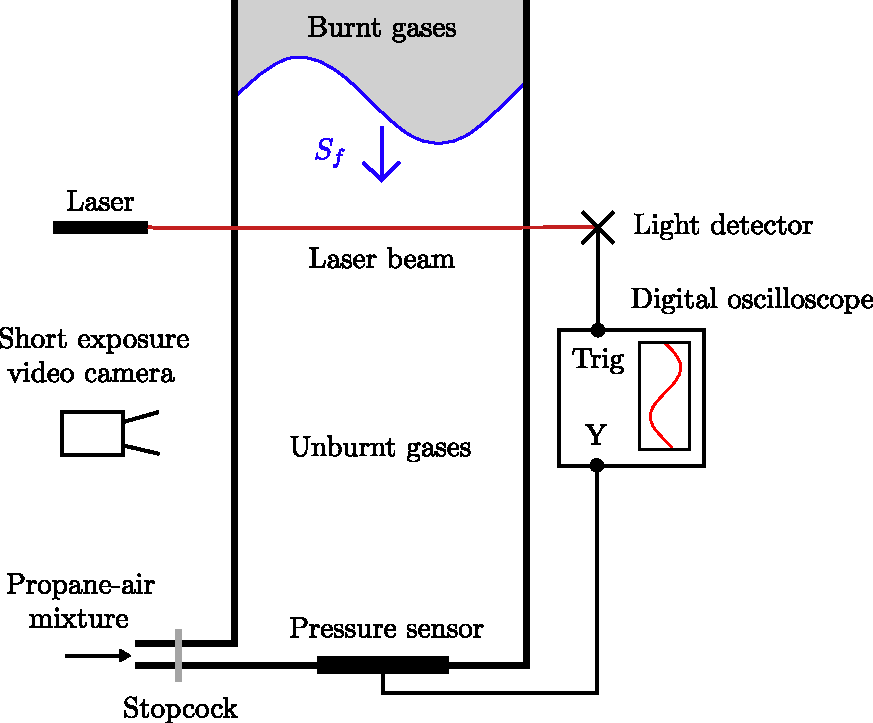
\includegraphics[scale=0.6]{assets/imgs/Searby-92.pdf}
\caption{Illustration of the experimental apparatus of \cite{searby1992AcousticInstabilityPremixed}.}
\label{fig:searby-experiment}
\end{figure}

An insightful experiment into thermoacoustics was performed later in 1992 by Searby \cite{searby1992AcousticInstabilityPremixed} and studied relationships between a cylindrical tube's acoustics as well as the speed and shape of the premixed flame within. The experimental apparatus is depicted in \fig{fig:searby-experiment}. Propane-air mixtures were lit at the top end of the tube and propagate down, with any acoustic disturbance detected by a pressure sensor at the bottom. Additionally, a small laser beam was place near the top of the tube to detect the flame as thermal gradients deflect the light. This triggers a digital oscilloscope to record pressure disturbances from the pressure sensor. A short exposure video camera was used to image the flame surface and observe its structure as it propagates. Since propane (C$_3$H$_8$) is a relatively heavy fuel with a species diffusion rate lower than methane's, the lean and stoichiometric mixtures used have Lewis numbers which are never below the critical Lewis number, $\Le_\rm{crit}$, required for \emph{thermodiffusive instabilities} \cite{zeldovich1944TheoryCombustionDetonation,barenblatt1962DiffusionalThermalStabilIty,sivashinsky1977DiffusionalThermalTheoryCellular} to have an effect. Note that the downward propagating flames will have been somewhat stabilised by the \emph{Rayleigh-Taylor} (RT) instability. The primary instability is observed alongside a secondary, which is associated with a different feedback mechanism, acoustic envelopes and flame dynamics.

\begin{figure}[t]
\centering
\begin{subfigure}{0.49\textwidth}
\centering
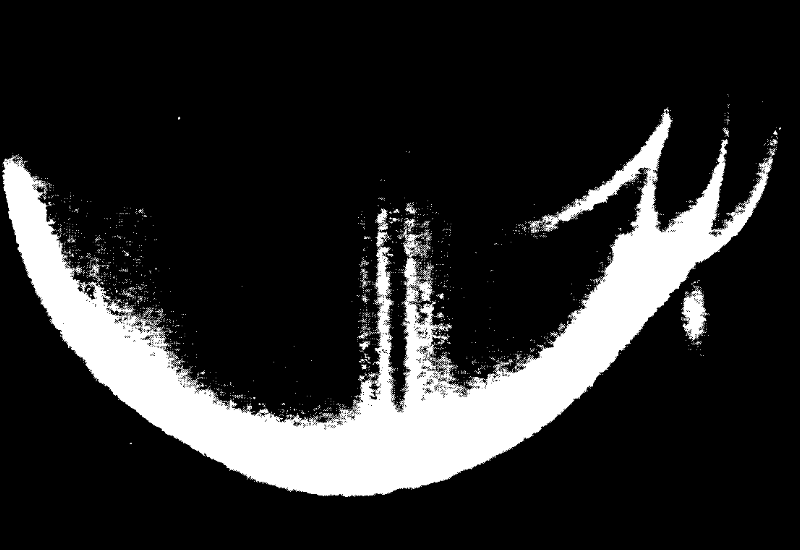
\includegraphics[height=5cm]{assets/imgs/Searby-92-flame_a.png}
\caption{}
\label{fig:Searby-92_flames_a}
\end{subfigure}
\hfill
\begin{subfigure}{0.49\textwidth}
\centering
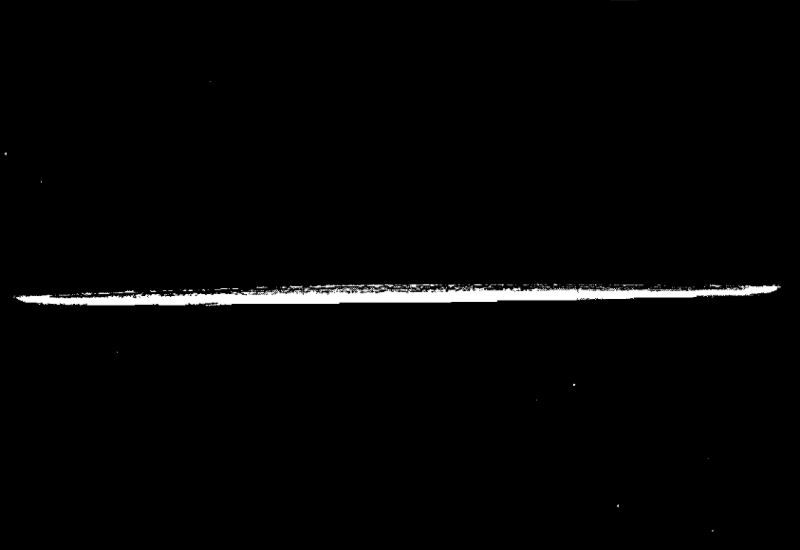
\includegraphics[height=5cm]{assets/imgs/Searby-92-flame_b.png}
\caption{}
\label{fig:Searby-92_flames_b}
\end{subfigure}

\vspace*{3mm}

\begin{subfigure}{0.49\textwidth}
\centering
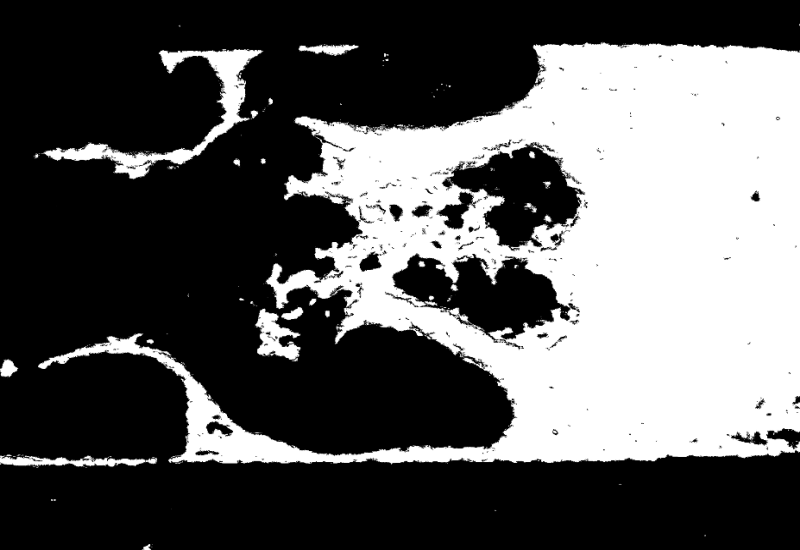
\includegraphics[height=5cm]{assets/imgs/Searby-92-flame_c.png}
\caption{}
\label{fig:Searby-92_flames_c}
\end{subfigure}
\hfill
\begin{subfigure}{0.49\textwidth}
\centering
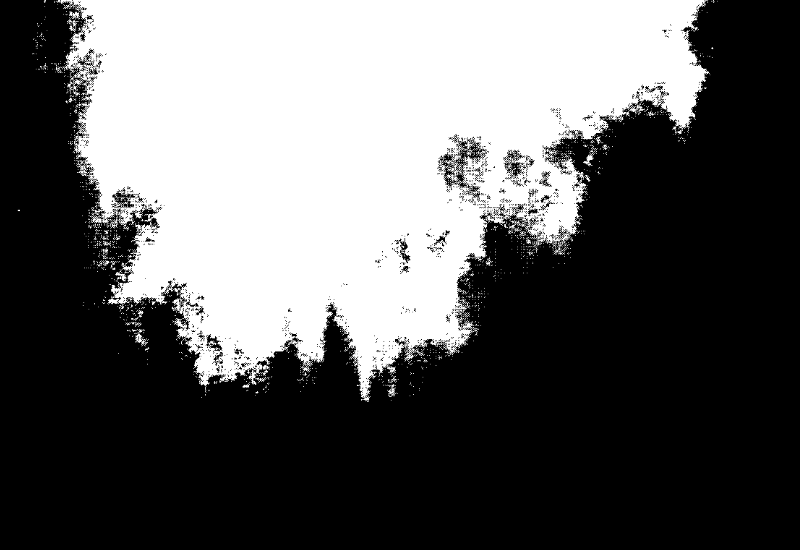
\includegraphics[height=5cm]{assets/imgs/Searby-92-flame_d.png}
\caption{}
\label{fig:Searby-92_flames_d}
\end{subfigure}
\caption{Photos, courtesy of \cite{searby1992AcousticInstabilityPremixed}, of flames at different stages of TA response. (a) shows the characteristic curved shape of a hydrodynamically unstable flame before any acoustics are significantly effecting the flame shape. (b) is a flame flame under the effect of the primary TA instability. (c) shows a cross-sectional slice of a flame rotated by $90\degree$ under the secondary instability. (d) shows a flame after the breakdown of cellular structures, which leads to a self-turbulent flame.}
\label{fig:Searby-92_flames}
\end{figure}

Initially, the flame curves as a result of the hydrodynamic instability, as photographed in \fig{fig:Searby-92_flames_a}. After some time, the acoustic amplitude increases due to primary instability. As the acoustic amplitude increases the flame flattens, seen in \fig{fig:Searby-92_flames_b}, resulting in a decrease in flame speed due to the decreased fuel consumption rate. In some of the flames tested, only the primary instability is observed, but in some others it progresses beyond this to the secondary instability -- often before the fully flattened flame is observed. At the immediate onset of the secondary instability, if it occurs, a cellular structure of a given wavenumber appears and corresponds to a rapid increase in the acoustic amplitude. This onset is much more rapid than for the primary instability, and eventually the cellular structure transitions into a symmetric flame structure similar to \fig{fig:Searby-92_flames_c}. Provided the flame has not yet reached the end of the tube it may also devolve into a self-turbulent flame similar to that shown in \fig{fig:Searby-92_flames_d}. The flame structures resulting from the secondary instability have significantly higher velocities as a result of their massively increased flame surface area and are viewed as a violent instability. The self-turbulent regime marks a significant decline to the acoustic amplitude as there is no regular release of pressure fluctuations from the flame.
% Flat flame under primary can be seen as a limit cycle

The secondary instability mechanism is seen by Searby \cite{searby1992AcousticInstabilityPremixed} as a \emph{parametric instability}. Searby and Rochwerger \cite{searby1991ParametricAcousticInstability} pose this system as a Mathieu equation by incorporating the effect of acoustic force into an equation for flame position under the influence of gravity, which is otherwise written as a damped harmonic oscillator \cite{searby1986WeaklyTurbulentWrinkled}. The Mathieu equation demonstrates a canonical example of parametric instability, since solutions remain unbounded whenever the forcing acoustic frequency is double that of the natural frequency implied by the flame in its damped harmonic oscillation. Physically this corresponds to a flame with a structure that oscillates with a period double that of the acoustic period.

% EXPLAIN WHAT S_L AND L_TH ARE
\begin{figure}[t]
\centering
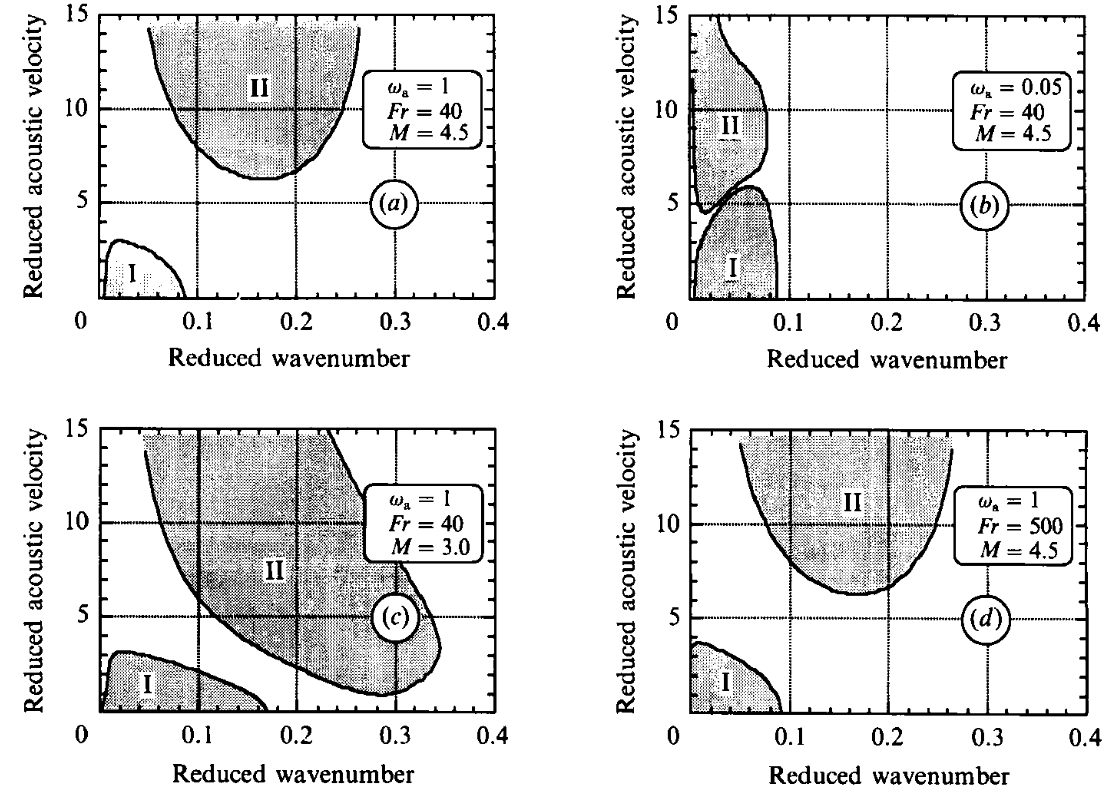
\includegraphics[height=11cm]{assets/graphs/thermoacoustic-stability.png}
\caption{Stability diagrams, courtesy of \cite{searby1991ParametricAcousticInstability}, for four different values of $ω_a$, $\Fr$ and $\Mk$. The regions I and II are regions of instability for the plane flame. Reduced wavenumbers are given as $k l_\rm{th}$ and reduced acoustic velocities are $u_a / S_L$.}
\label{fig:ta-stab}
\end{figure}

Using this formation of the flame front as solutions to the Mathieu equation, \cite{searby1991ParametricAcousticInstability} calculates regions of flame instability for a planar flame as functions of perturbation wavenumber $k$, acoustic velocity $u_a$ (the amplitude of which can be thought of as the intensity or volume of sound), acoustic frequency $ω_a$, Froude number $\Fr$ (representing non-dimensional inverse of gravitational forcing) and Markstein number $\Mk$ (a crucial flame parameter connecting the sensitivity of the flame's speed to perturbations to its surrounding hydrodynamics). They then plot these regions in \fig{fig:ta-stab}. Note that these plots do not acoustic instability mentioned above, but their effect on flame stability for a planar flame. In all the plots, there are two disjoint regions of flame instability. The region I represents hydrodynamic instability and occurs, as expected, at zero acoustic velocity for some wavenumber interval. This region ends at some finite $u_a$ as the primary acoustic instability eventually overcomes the hydrodynamic one. At non-zero acoustic velocity, region II of flame instability begins, corresponding to the aforementioned parametric instability. Interestingly, some of the graphs show acoustic velocities where regions I and II can coexist for different wavenumber intervals. In these cases, the primary thermoacoustic instability is expected to lead immediately into the secondary instability with no planar flame observed. On the other hand, for those acoustic velocities where neither region is present the planar flame is stable, so we see structures like \fig{fig:Searby-92_flames_b} where the flame has spontaneously flattened before any secondary instability can occur. We also notice that there is a wavenumber in region II which corresponds to the lowest unstable acoustic velocity. This means that once this acoustic velocity is met, only that wavenumber (and wavenumbers close to it) will be present as wrinkles in the flame. Finally, we note that the effect of increased gravity (decreased $\Fr$) on these downward propagating flames has stabilised the very low wavenumbers next to region I as the RT effect actually stabilises the plane flame.

An experiment was also performed by \cite{searby1991ParametricAcousticInstability} to demonstrate these results. A similar apparatus to \fig{fig:searby-experiment} was used, with significant changes being the usage of a loudspeaker in the bottom of the combustion tube to play sounds of wavelength one-quarter or three-quarters of the wavelength of the tube. A porous plate was placed above the loud speaker to remove any turbulence such that our laminar theories can be applied. Using the loud speaker to excite the flame at known volumes and frequencies (which correspond to controlling $u_a$ and $ω_a$, respectively), they observe both the planar and wrinkled flames described above. The sound intensity corresponding to the quietest parametrically unstable flame may then be plotted for a variety of acoustic frequencies, resulting in a curve predicted by the Mathieu equation model described above for a specific Markstein number. This enables the direct estimation of the Markstein number, which remains a difficult challenge and so remains a prevalent technique \cite{delfin2024ThermoacousticParametricInstability}.

Beyond this, TA oscillations have been observed in a variety of experimentation. Methane-air combustion in a cylindrical tube was investigated experimentally in \cite{fichera2001ExperimentalAnalysisThermoacoustic} with data recorded from an optical sensor to detect changes to heat release, a pressure transducer for internal pressure recordings and a microphone for external pressure recordings. TA oscillations were observed and a non-linear analysis into the dynamical behaviour of the flame recordings demonstrate a chaotic nature to these thermoacoustics. The global stability of the flame, which is guaranteed by diffusive effects, is corroborated via calculation of the set of Lyapunov exponents. The thesis \cite{ebieto2017DynamicsPremixedFlames}, provides a detailed setup to gather high-speed imagery, chemiluminescent and pressure data in a variety of TA flames. The effects of a variety of phenomena affecting acoustic stability, such as RT instability, are outlined. Further experimentation is done on premixed flame oscillations in \cite{delfin2024VideoTransientParametric,martinez-ruiz2018VideoPremixedflameOscillations,delfin2024ThermoacousticParametricInstability} and provide high-fidelity imagery of flames under the effects of primary and secondary instability in \cite{delfin2024VideoTransientParametric,martinez-ruiz2018VideoPremixedflameOscillations}.





\subsection{Thermoacoustic Instability Modelling}

\begin{figure}[t]
\centering
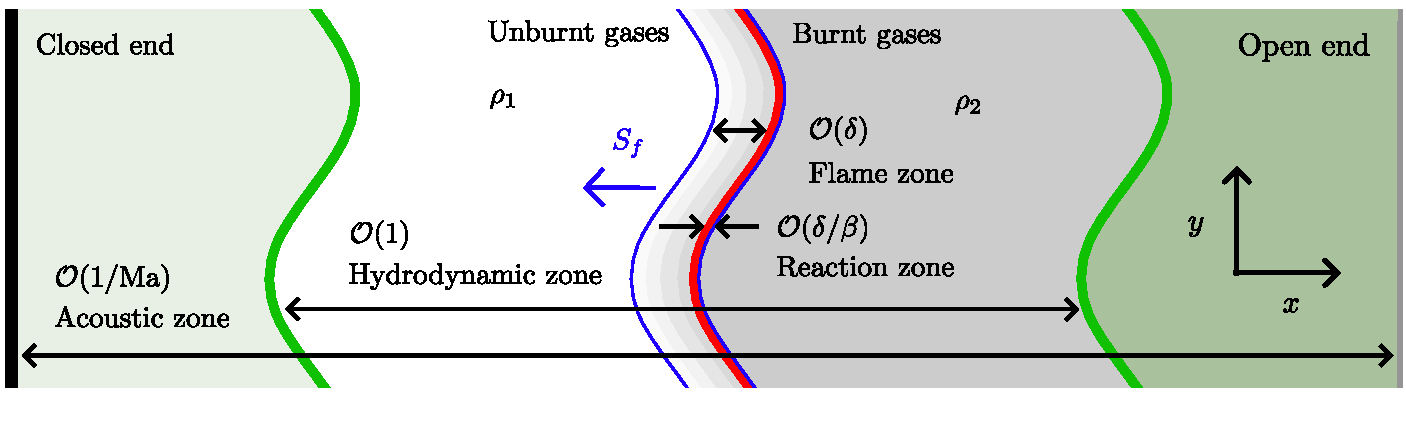
\includegraphics[scale=0.6]{assets/imgs/AW-flame.pdf}
\caption{Diagram showing the model geometry of the multiscale analysis performed by \cite{assier2014LinearWeaklyNonlinear}. The different non-dimensionalised asymptotic scales involved in the full analysis are labeled above the domain.}
\label{fig:AW-flame}
\end{figure}

Later on, work by Assier and Wu \cite{assier2014LinearWeaklyNonlinear} studied the stability of a \emph{flame-flow-acoustic} system, where a freely propagating flame in a closed-open, periodic duct is considered. \fig{fig:AW-flame} illustrates this geometry and is reminiscent of the experimental domain shown in \fig{fig:searby-experiment} of \cite{searby1992AcousticInstabilityPremixed}, excluding any wall boundary layer effects. Results from hydrodynamic flame theory \cite{matalon1982FlamesGasdynamicDiscontinuities,clavin1982EffectsMolecularDiffusion} are used to separate the dynamics within the flame from the outer fluid. This outer region is then separated into the usual $\cl{O}(1)$ hydrodynamic zone and a far-away $\cl{O}(1/\Ma)$ acoustic zone. Further asymptotic analysis is performed in the flame reference frame, coupling the two regions through dynamic jump conditions. A weak non-linearity assumption is made to simplify the flame equation such that linear stability analysis may be performed about the steady solutions to the Michelson-Sivashinsky equation \cite{sivashinsky1977NonlinearAnalysisHydrodynamic,michelson1977NonlinearAnalysisHydrodynamic,matalon2018DarrieusLandauInstability}.

They find that, when the acoustic interaction is included, these solutions are no longer linearly stable and the maximum growth rate of this instability increases significantly with heat release $q$. Non-linear stability analysis is also performed using a solver for the flame position coupled to the dynamical acoustic jump conditions. This is compared to the results of \cite{searby1992AcousticInstabilityPremixed} and they find they are able to qualitatively reproduce the primary instability and the onset of the secondary instability provided the flame parameter is allowed to deviate from its predicted value. In the latter case, the unsteady nature of the acoustic coupling to the flame induces an unsteady RT effect as the acoustic acceleration oscillates into and away from the less dense products. This is viewed as the driving mechanism behind this parametric instability. In a later conference paper, \cite{assier2014CombustionInstabilityModel}, tangential velocity terms are reintroduced and the parameter resulting in the same flame and acoustic behaviour as seen in \cite{searby1992AcousticInstabilityPremixed} more closely match the expected value. These results are surprisingly fruitful given they assume weak non-linearity in the face of the large heat releases the model is tested against.

In \cite{jun2023ParametricInstabilityPropagating} the secondary instability in hydrogen enriched methane-air flames is studied numerically in an open-ended tube. The structure of their flames under the full non-linear effect of the secondary instability is an impressive match to the experiment of \cite{ebieto2017DynamicsPremixedFlames}, in spite of a lack of convergence in the phase of sub-harmonic oscillations to the flame front (between grid spacings of 100 $μ$m to 50 $μ$m). They also find that the Rayleigh Index, $\rm{RI}$ is a good indicator for the onset of the secondary instability and that the violent acoustic output of this parametric instability may also be attributed to the changes in flame surface area strengthening oscillations in heat release which cause the thermoacoustic effect. They determine the main reason secondary instability is not seen in simulations of faster flames is simply that the tube is not long enough for the instability to develop before the flames reach the end of the tube. This validates a desire to model the behaviour of flames which are held in place, such as those in a held in place by combustor geometry in counterflow.


% veiga-lopez2020ThermoacousticAnalysisLean
% - Experimental study of H2-air flames in Hele-Shaw cells
% - Study effects of confinement due to cell geometry, gravity and mixture composition on thermoacoustic oscillations
% - Heat loss effects are most prevalent for very thin cells, where ...




\subsection{G-Equation Model}

% Aimee morgans




\subsection{Low-Order Thermoacoustic Modelling}

% n-tau models
% control theory stuff i don't understand

\cite{juniper2018SensitivityNonlinearityThermoacoustic}




\subsection{Instability Control}

\begin{figure}[t]
\centering
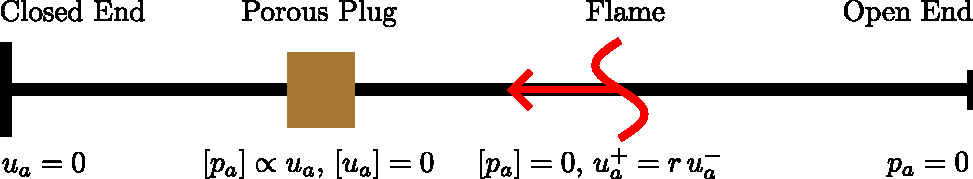
\includegraphics[scale=0.6]{assets/imgs/GP-model.pdf}
\caption{Illustration of the one-dimensional model considered by \cite{gaton-perez2025MitigationThermoacousticInstabilities}, where boundary conditions for each component of the model are shown.}
\label{fig:GP-model}
\end{figure}

Simpler analysis is performed by Gatón-Pérez et al. \cite{gaton-perez2025MitigationThermoacousticInstabilities} to evaluate the eigenstates of a one-dimensional closed-open tube containing a porous plug and a flame. Using Darcy's law to model the plug and assuming linear acoustics, the acoustic eigenmodes of the tube are found numerically. Experimental data is then compared against the one-dimensional model depicted in \fig{fig:GP-model}, where the heat release parameter, thermal length scale and the plug's permeability set by experimental values. Effects of heat losses through the combustor walls is given by \cite{flores-montoya2022NonadiabaticModulationPremixedflame}. The model is able to predict the flame locations within the tube which are most likely to trigger thermoacoustic resonance despite no consideration of the flame's motion or its thermal response to acoustics being made. These are the locations where the resulting acoustic eigenmodes have the lowest decay imposed by the porous plug. In this way, they show experimentally that the location of the porous plug may be chosen to preferentially mitigate different frequencies and reduce the likelihood of thermoacoustic instability. Evidently though, a simple one-dimensional model of this ilk is restricted in application to strongly one-dimensional, ducted combustors. As soon as a broader combustor or plenum is used, the two-dimensional acoustics (e.g. Helmholtz modes) must also be considered.

% luzzato2015ModellingControlCombustion (THESIS)

% liao2025ActiveControlThermoacoustic

% meadows2015PorousInsertsPassive

% mcmanus1993ReviewActiveControl




\subsection{Intrinsic Thermoacoustic Feedback}

\begin{figure}[t]
\centering
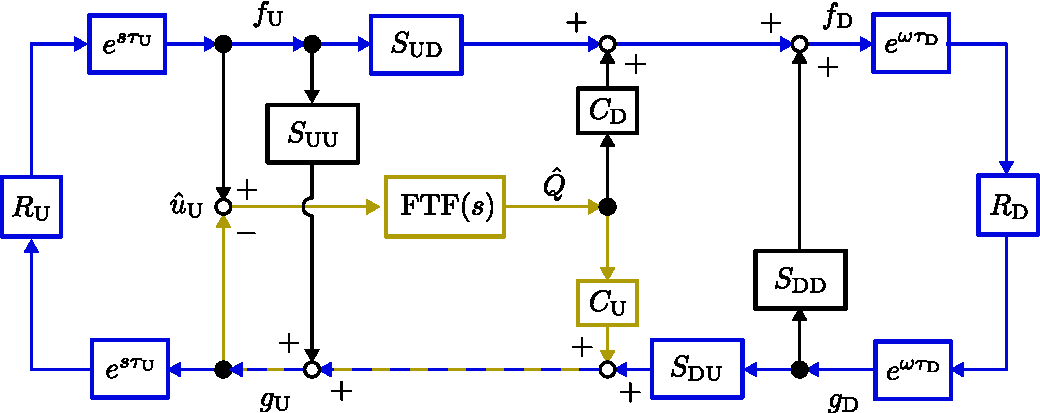
\includegraphics[scale=0.65]{assets/imgs/ITA-mech.pdf}
\caption{INTRINSIC THERMOACOUSTIC FEEDBACK LOOP}
\label{fig:ita-loop}
\end{figure}

% Doesn't need to be too elaborate!

% But there are not just acoustic modes, the full set of thermoacoustic instability modes includes ITA too [cite?]
% explain feedback loop
% phasors are cool
% some other stuff i read about
% cite the good reviews!

\cite{emmert2015IntrinsicThermoacousticInstability}
\cite{silva2023IntrinsicThermoacousticInstabilities}
\cite{hoeijmakers2014IntrinsicInstabilityFlame}
\cite{hoeijmakers2016FlameDominatedThermoacoustic}
\cite{orchini2025TrackingAcousticIntrinsic}
\cite{chen2024BiglobalLinearStability}
% Polifke?






\section{Techniques for Computational Fluid Dynamics (CFD)}

% Mention AVBP and CERFACS?

\cite{, domingo2023RecentDevelopmentsDNS, chen2011PetascaleDirectNumerical, yang2015LargeEddySimulationPresent, veynante2002TurbulentCombustionModeling, moin1998DirectNumericalSimulation, tennekes1972FirstCourseTurbulence}

The most brute force way to simulate a fluid system would be one where you try to accurately simulate every detail involved in the fluid. This idea was first studied by Orszag \cite{orszag1970AnalyticalTheoriesTurbulence}, where he defines \emph{direct numerical simulations} (DNS) as a numerical simulation with enough grid points to full resolve the smallest physical phenomena in the system. Originally, Orszag studied this in the context of turbulent flows. In turbulent flows, we have vortices not only on the order of the typical flow length scale $l_T$, called the integral length scale, but also of sizes all the way down to the smallest turbulence scale known as the kolmogorov length scale $l_K$ [CITE], where the rate at which viscous dissipation effects dampen vortices far exceeds the inertial forces of the vortex. In DNS of turbulent combustion, the smallest scale vortices must be resolved in addition to the smallest chemical length scales. In this context, the relevant time scales are chemical $τ_C = l_{\rm{th}} / S_L$, integral $τ_T = l_T / u'$ and Kolmogorov $τ_K = l_K / u'$ given an RMS velocity scale $u'$. Hence, the number of degrees of freedom required to resolve a three-dimensional box of size $L$ is:
\begin{equation}
N_{\rm{tot}} = \left( \frac{L}{2 l_T} \right)^3 \, \Da \, \Ka \, \rm{Re}_T^{7 / 4}
\end{equation}
where we define the turbulent Reynolds, Damköhler and Karlovitz numbers by:
\begin{equation}
\rm{Re}_T \equiv \left( \frac{l_T}{l_K} \right)^{4 / 3},
\quad
\Da \equiv \frac{τ_T}{τ_C}
\quad \text{and} \quad
\Ka \equiv \frac{τ_C}{τ_K}
\end{equation}
respectively.


For most turbulence intensities and combustion reactions, this means having a discretisation length scale on the order of 10 - 100 $μ$m.

% The size of this kolmogorov length scale is determined by the turbulent reynolds number and the integral scale with the relationship

% A consequence of this is the extraordinary computational cost to accurately simulate a large domain. To fully resolve DNS of turbulent combustion, for example, the small chemical length scale must be resolved in addition to the smallest scale vortices. 

% An alternative method that is widely used is LES and involves using models to estimate the transfer of energy at the smallest scale rather than fully simulating them [cite les review: Yang 2015]
% DNS for turbulent combustion are reviewed in \textbf{Domingo and Vervisch 2023} (with connection to LES) and \textbf{Chen 2011}.

% For small-scale, low-speed methane-air and hydrogen-air combustion, the flows we look at have similar properties to air, so are not very viscous meaning the smallest scale vortices in a fully developed turbulent may be ~...?
% But the turbulence usually isn't our biggest worry, since we also have the thin region that the reaction is taking place to resolve, usually only 300 {\textmu}m which is resolved with ~15 nodes in a high order code
% Regardless, when performing DNS careful consideration must be made to use ample sample points

% ?? DNS with simple transport / chemical schemes?

\subsection{Mesh-free Methods}

\cite{monaghan1992SmoothedParticleHydrodynamics, vacondio2021GrandChallengesSmoothed}





\subsection{High-Order Discretisation}




\subsection{Navier-Stokes Characteristic Boundary Conditions}

\cite{thompson1987TimeDependentBoundary, thompson1990TimeDependentBoundaryConditions, poinsot1992BoundaryConditionsDirect, poinsot2005TheoreticalNumericalCombustion, sutherland2003ImprovedBoundaryConditions}

% [Thompson 1987, 1990, Poinsot and Lele 1992, Sutherland and Kennedy 2003, Poinsot and Veynante 2005]


% Many types of boundary conditions may be chosen for combustion schemes:
%% Periodic are very simple to enforce numerically so require no elaboration
%% No-slip or slip wall conditions
%% isothermal or adiabatic walls
%% acoustically reflecting or non-reflecting walls or inflow / outflow
%% In the case of inflow / outflow many more cases

% In most of these cases, we can use the formalism called characteristic boundary conditions (characteristic BCs)




% The simplest boundary conditions, i.e. those with constant (Dirichlet) boundary values (p=const), usually reflect acoustic waves back toward the interior of the domain. For most situations we want to simulate, this doesn't represent the physical situation, where we would rather pretend the medium continues outside of the computational domain. This motivates a need for boundary conditions which do not reflect acoustic waves - non-reflecting boundary conditions. The formalisms are based of characteristic waves entering / leaving the domain

% Fixed velocity inlets give full reflections, so cannot be used in a non-reflecting case.

% Immersed boundary methods are also an option and open up possibilities for boundaries not restricted specific node placement, especially for moving boundaries. But as detailed in King 2022, these a largely restricted to lower order accuracy at these boundaries (cite, and for what reason?).



\subsection{Delayed-Time Domain Impedance Boundary Conditions}


% Describe TDIBC briefly before going into time delay model!


\begin{figure}[t]
\centering
\includegraphics[scale=0.65]{example-image-a}
\caption{D-TDIBC}
\label{fig:D-TDIBC}
\end{figure}

Although many variations on TDIBC exist, the \emph{Delayed-Time Domain Impedance Boundary Conditions} (D-TDIBC) of \cite{douasbin2018DelayedtimeDomainImpedance} are particularly relevant for the simulation of thermoacoustic instabilities. By modelling the effect of an acoustic time delay, $τ$, a part of the computational domain -- say, an exhaust pipe -- may be truncated in place of a numerical boundary. Then, the response of this new boundary to incoming acoustics should be a sinusoidal Moiré pattern in the frequency domain. The proposition of \cite{douasbin2018DelayedtimeDomainImpedance} is that this pattern may be modelled via a meromorphic function of $2n$ simple poles. The location of these poles and their residues are then found in a preprocessing step as the values which minimise the least-squares fit with the desired response curve. Each time step then, the resulting constants are used to evaluate the change in acoustic variable at the boundary in such a way that no memory of previous time steps are required. 

After validating the model by testing its response to a Gaussian pressure bump, the model is compared against DNS of methane-air combustion in a 2D flame holder, where the upstream end is closed and the downstream end is open. Comparing this to DNS where the last 25 cm at the downstream end has been truncated to use D-TDIBC, they find that the time delay model accurately recovers the one-, three- and five-quarter eigenmode shapes, with small quantitative errors in their sound spectra. Considering the $\sim 13\%$ reduction in degrees of freedom in the computational domain resulting from the truncation, this can be seen as an impressive recovery of the problem's physics by using what is essentially a one-dimensional low-order model in the truncated region for the acoustics. Since the model constants are calculated as a preprocessing step, the envelope of the acoustic response in the frequency domain may essentially be changed arbitrarily, presenting a benefit in case different pass bands are desired.

Besides the inevitable drawbacks stemming from: the low-order model's inaccuracy and the requirement of a strongly one-dimensional flow at the boundary to match this model, other drawbacks remain prevalent. For one, no method to visualise acoustics residing in the fictitious, truncated domain is provided, potentially leading to a \emph{black-box} of energy where acoustics are essentially stored, but not known. For another, the preprocessing steps are required for each value of $τ$ used. So, if the time delay were to change dynamically during the simulation (e.g. due to an expanding computational domain to ensure the flame remains within), this preprocessing may happen each step, becoming computationally costly.






\cleardoublepage

\chapter{Simulation Methodology} \label{ch:dns-methods}
\section{The SUNSET Combustion Code}

For the simulations performed in the remainder of this report, we use the \emph{Scalable Unstructured Node-SET} (SUNSET) code \cite{kingSunsetFlames,king2024MeshFreeFrameworkHighOrdera}, to perform DNS of the governing equations (described in \chap{ch:combust-model}) with high accuracy in domains of arbitrary complex geometries and highly variable node densities. That it is DNS allows us to simulate turbulent combustion without requiring any model for the subgrid-scale vortices present in turbulent flows. For the simulations performed in \chap{ch:results} we actually simulate laminar, not turbulent flows, but the simulation code nevertheless provides high accuracy discretisations such that discretisation error is reliably minimised. The method used to this end is the \emph{Local Anisotropic Basis Function Method} (LABFM), and is explained thoroughly in the proceeding section. Boundary conditions are provided via the \emph{Navier-Stokes Characteristic Boundary Conditions} (NSCBC) formalism, and are detailed in \sect{sec:NSCBC}.

Time integration makes use of the explicit Runge-Kutta scheme denoted as RK3(2)4[2R+]C under the classification of \cite{kennedy2000LowStorageExplicitRunge}, which is a third order, low storage (only requiring two or three registers per field per node), four step method in time with embedded second order error estimation. Even under turbulent combustion, error accumulated in time stems primarily from spatial detail (such as thin reacting zones, small Kolmogorov vortices etc.) rather than temporal dynamics (such as the vortex energy cascade, acoustics and diffusion). Thus, a third order error correcting scheme is suitable and our focus remains on the discretisation scheme used.

To ensure the stability of numerical solution, time steps $δ t$ are chosen dynamically. Specifically, such that the fastest travelling information in the solution may travel only $\cl{O}(δ x)$ where $δ x$ is the discretisation length scale \cite{courant1928UeberPartiellenDifferenzengleichungen}. Considering only the travelling of acoustic waves and diffusion terms through a computational domain of nodes $\vb{x}_i$ for $i \in \cl{I}$:
\begin{equation} \label{eqn:dt-stab}
\boxed{
\delta t = \min_{i\,\in\,\cl{I}}\left[ \min \left( C_{\rm{aco}} \frac{δ x_i}{|\vb{u}_i| + c_i}, \: C_{\rm{mom}} \frac{δ x_i^2}{\cl{D}_{\rm{mom}, i}}, \:  C_{\rm{sp}} \frac{δ x_i^2}{\min_α \cl{D}_{α, i}}, \: C_{\rm{th}} \frac{δ x_i^2}{\cl{D}_{\rm{th}, i}} \right) \right]
}
\end{equation}
where a subscript $i$ represents the value of that field at node $\vb{x}_i$. Variables $\cl{D}_{\rm{mom}, i}$, $\cl{D}_{α, i}$ and $\cl{D}_{\rm{th}, i}$ are local diffusion scales corresponding to viscosity, species mass transport and heat diffusion:
\begin{equation}
\cl{D}_{\rm{mom}} = \frac{μ}{ρ}, \quad \cl{D}_{α} = D_α, \quad \cl{D}_{\rm{th}} = \frac{λ}{ρ c_p},
\end{equation}
and the constants $C_\rm{aco}$, $C_\rm{mom}$, $C_\rm{sp}$ and $C_\rm{th}$ are determined separately by the stability of time integrator.

Parallelism is primarily implemented via domain decomposition, exploiting the local nature of the discretisation method by splitting the domain into $N_{\rm{procs}}$ smaller sub-domains used by each of the $N_{\rm{procs}}$ processors. Under the architecture of a distributed system, each processor stores data of the nodes in its subdomain and information is passed between processors via the MPI \cite{walker1996MPIStandardMessage} standard where needed. Load balancing is achieved simply by ensuring the number of nodes per processor is roughly the same. Due to the size of stencils required by LABFM, there is a minimum size of roughly 1000 nodes per processor, meaning there is a practical maximum number of processors which may be used to parallelise the simulation of a given  computational domain discretisation.




\section{The Local Anisotropic Basis Function Method}
\sectionmark{LABFM}

LABFM \cite{king2024MeshFreeFrameworkHighOrder, king2020HighOrderDifference, king2024MeshFreeFrameworkHighOrdera, king2022HighOrderSimulationsIsothermal, broadley2025HighorderMeshfreeDirect, starepravo2025CanNeuralNetworks} is a high order spatial method used particularly in the computation of fluid flows. It allows for the calculation of arbitrary order approximations to spatial derivatives with arbitrary orders of accuracy, all on unstructured, mesh-free node sets. In keeping with the tradition set forth in prior methods (e.g. finite differences), polynomial interpolation is used as a first step before making derivative approximations. Specifically, we choose to set out the method in the context of making a high order interpolation based off finitely many discrete function values $φ_j$, before extending this to high-order derivatives, where further assumptions can be made to simplify derivation


\subsection{High-Order Interpolations}

Consider a location $\vb{x}$ surrounded locally by finitely many nodes $\vb{x}_j$ which are enumerated by $j \in \cl{N}(\vb{x})$, where $\abs{\vb{x} - \vb{x}_j} < h(\vb{x})$ for all $j$. Assume the field $φ(\vb{x})$, which is only known at the points $φ_j = φ(\vb{x}_j)$, is smooth enough.\footnote{Such that as many derivatives of $φ$ as are used in the derivation below are available to us.} Then, we express the interpolated value $φ(\vb{x})$ as a linear combination of the surrounding values $φ_j$:
\begin{equation} \label{eqn:L}
L^{\rm{int}}[φ](\vb{x}) \equiv \sum_{j \in \cl{N}(\vb{x})} φ_j w^{\rm{int}}(\vb{x}, \vb{x}_j) \approx φ(\vb{x}).
\end{equation}
To find the weights $w^{\rm{int}}(\vb{x}, \vb{x}_j)$, we will be evaluating $φ_j$ by means of Taylor series via derivatives of $φ$. Each derivative is a projection from the vector of derivatives of $φ$:
\begin{equation}
\vv{D}[φ] = \left(φ, \pdv{φ}{x}, \pdv{φ}{x}, \pdv[2]{φ}{x}, \pdv[2]{φ}{x}{y}, \pdv[2]{φ}{x}, \dots \right)^T
\quad \text{and} \quad
\vv{D}^k[φ] = \left(φ, \pdv{φ}{x}, \pdv{φ}{x}, \dots, \pdv[k]{φ}{x}, \dots, \pdv[k]{φ}{y} \right)^T,
\end{equation}
where we have assumed that $φ$ is a scalar field over two spatial dimensions $\vb{x}=(x, y)$, although the method may be simply extended to any number of dimensions (with the caveat that the number of nodes required increases greatly with dimension). In this notation, interpolation becomes $φ(\vb{x}) = \vv{D}[φ](\vb{x}) \cdot \vv{C}^{\rm{int}} = \vv{D}^k[φ](\vb{x}) \cdot \vv{C}^{\rm{int}, k}$ where $\vv{D}[φ](\vb{x})$ is the vector $\vv{D}[φ]$ evaluated at the location $\vb{x}$, $\vv{C}^{\rm{int}} = (1, 0, 0, 0, 0, 0, \dots)^T$ and $\vv{C}^{\rm{int}, k} = (1, 0, 0, \dots, 0)^T$, is of the same length as $\vv{D}^k$. Introducing the vectors of monomials:
\begin{equation}
\vv{X}(\vb{x}) = \left(1, x, y, \frac{1}{2!} x^2, xy, \frac{1}{2!} y^2, \dots \right)^T
\quad \text{and} \quad
\vv{X}^k(\vb{x}) = \left(1, x, y, \dots, \frac{1}{k!} x^k, \dots, \frac{1}{k!} y^k \right)^T.
\end{equation}
we can simplify down the Taylor expansion of $φ$ around the point $\vb{x}$ for any $\vb{x}_j$ as:
\begin{subequations}
\begin{align}
φ_j &= φ(\vb{x}) + \pdv{φ}{x}\bigg|_{\vb{x}} (x_j - x) + \pdv{φ}{y} \bigg|_{\vb{x}} (y_j - y)  \\
& \qquad  \quad \ \, + \frac{1}{2!} \pdv[2]{φ}{x}\bigg|_{\vb{x}} (x_j - x)^2 + \pdv[2]{φ}{x}{y}\bigg|_{\vb{x}} (x_j - x) (y_j - y) + \frac{1}{2!} \pdv[2]{φ}{y}\bigg|_{\vb{x}} (y_j - y)^2 + \dots \\
&= \vv{D}[φ](\vb{x}) \cdot \vv{X} (\vb{x}_j - \vb{x}).
\end{align}
\end{subequations}
This may be truncated to $φ_j \approx \vv{D}^k[φ](\vb{x}) \cdot \vv{X}^k (\vb{x}_j - \vb{x})$ with $\cl{O}(h^{k + 1})$ truncation error. Hence, $k$ can be reinterpreted as the maximum order of polynomials $φ(\vb{x})$ under this approximation which are exactly interpolated.

Rewriting \equ{eqn:L} in this formulation:
\begin{subequations}
\begin{align}
L^{\rm{int}}[φ](\vb{x}) &= \vv{D}[φ](\vb{x}) \, \cdot \sum_{j \in \cl{N}(\vb{x})} \vv{X} (\vb{x}_j - \vb{x}) w^{\rm{int}}(\vb{x}, \vb{x}_j) \\
&\approx \vv{D}^k[φ](\vb{x}) \, \cdot \sum_{j \in \cl{N}(\vb{x})} \vv{X}^k (\vb{x}_j - \vb{x}) w^{\rm{int}}(\vb{x}, \vb{x}_j) \equiv \vv{D}^k[φ](\vb{x}) \cdot \vv{B}^{\rm{int}, k}(\vb{x}) \\
&\approx \vv{D}^k[φ](\vb{x}) \cdot \vv{C}^{\rm{int}, k}
\end{align}
\end{subequations}
So our problem now involves finding values of $w^{\rm{int}}(\vb{x}, \vb{x}_j)$ such that the \emph{vector of moments} $\vv{B}^{\rm{int}, k}(\vb{x})$ of $w^{\rm{int}}$ approximates $\vv{C}^{\rm{int}, k}$. For consistency, then, we require that the first component is independent of $h$:
\begin{equation}
1 = C^{\rm{int}, k}_0 \approx B^{\rm{int}, k}_0(\vb{x}) = \sum_{j \in \cl{N}(\vb{x})} w^{\rm{int}} (\vb{x}, \vb{x}_j),
\end{equation}
so $w^{\rm{int}} = \cl{O}(h^0)$, where the subscript zeroes represent the leading vector component. The resulting error in this approximation is the combined $\cl{O}(h^{k + 1})$ error of truncating the Taylor expansion of $φ_j$ and approximating $w^{\rm{int}}$.

What's left is to find the weights of $w^{\rm{int}}$ for any point $\vb{x}$ and nodes $\vb{x}_j$. To do this, we separate $w^{\rm{int}}$ into some dependence of $\vb{x}$ on the anisotropic surrounding nodes from the action of interpolation, which will later be generalised to arbitrary derivatives. This is done by writing it as the weighted sum of some anisotropic basis functions:
\begin{equation}
w^{\rm{int}}(\vb{x}, \vb{x}_j) = \vv{W}^k(\vb{x}_j - \vb{x}) \cdot \vv{\Psi}^{\rm{int}, k}(\vb{x})
\end{equation}
where the anisotropy is seen in the dependence of $\vv{W}^k$ on $(\vb{x}_j - \vb{x})$ rather than $|\vb{x}_j - \vb{x}|$ (contrasting to the radial basis function, RBF, method). Assuming that $\vv{W}^k$ comprises some suitable \emph{anisotropic basis functions} (ABFs) \cite{king2022HighOrderSimulationsIsothermal}, we must find the vector of weights $\vv{\Psi}^{\rm{int}, k}(\vb{x})$. This is done by substituting the new form into the vector of moments:
\begin{align}
\vv{C}^{\rm{int}, k}
\approx \vv{B}^{\rm{int}, k}(\vb{x})
= \left( \sum_{j \in \cl{N}(\vb{x})} \vv{X}^k (\vb{x}_j - \vb{x}) \otimes \vv{W}^k(\vb{x}_j - \vb{x}) \right) \cdot \vv{\Psi}^{\rm{int}, k}(\vb{x})
\equiv M(\vb{x}) \, \vv{\Psi}^{\rm{int}, k}(\vb{x})
\end{align}
where $M$ is a $n \times n$ matrix and $n$ is the number of components of $\vv{C}^{\rm{int}, k}$. The vector of weights $\vv{\Psi}^{\rm{int}, k}(\vb{x})$ is found when the linear system is solved. Carrying over the error terms from previous steps, we expect convergence on the order $(k + 1)$ as long as the matrix $M$ is well-posed and the values of nodes $\vb{x}_j$ are close enough to $\vb{x}$ such that $h$ is small.


\subsection{High-Order Derivatives}

\begin{figure}[t]
\centering
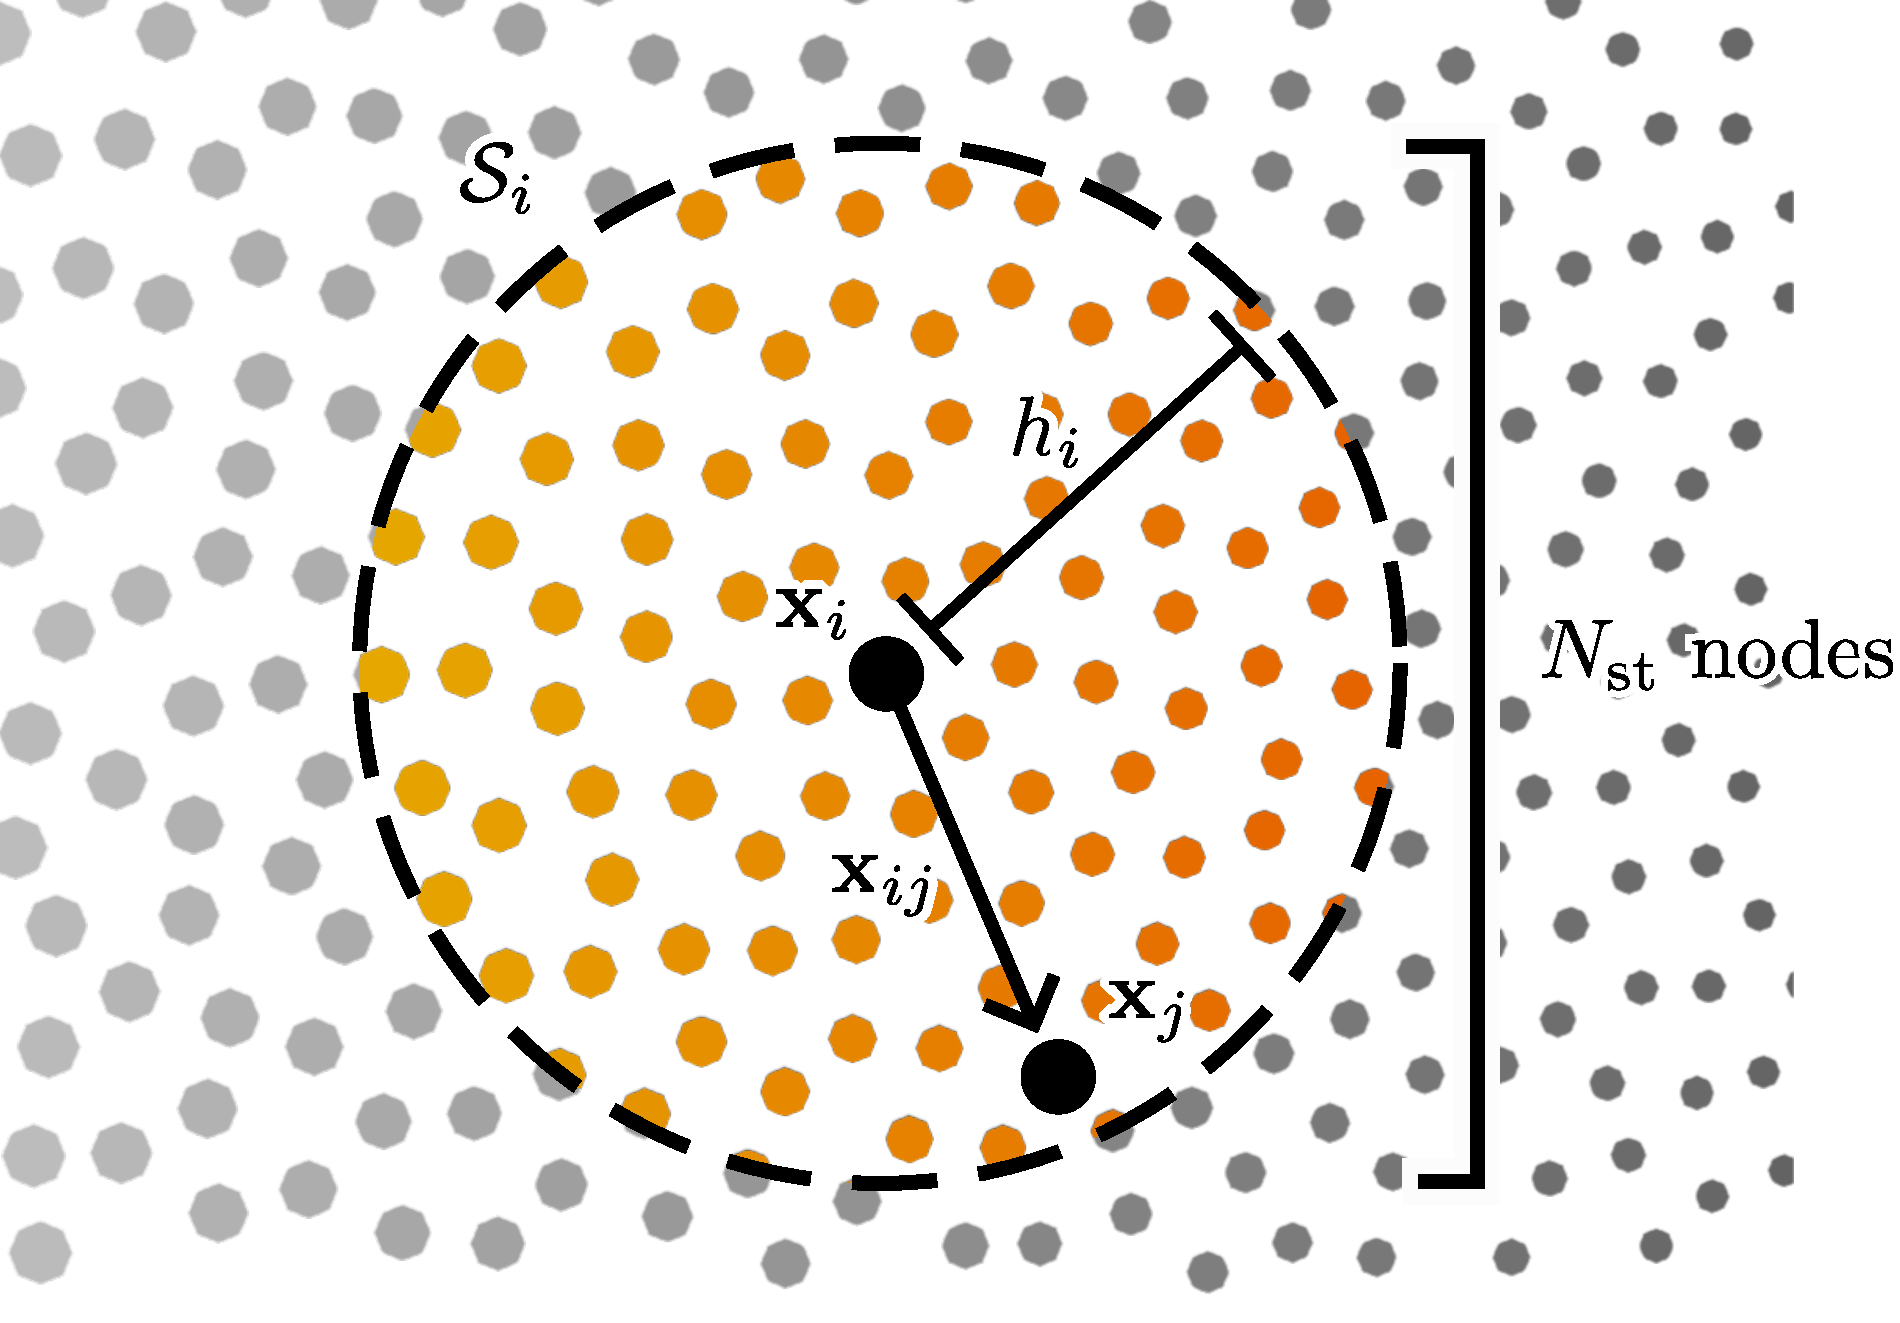
\includegraphics[scale=0.25]{assets/imgs/labfm-stencil-drawn_simple.pdf}
\caption{A example LABFM node discretisation and stencil.}
\label{fig:labfm-stencil}
\end{figure}

If we choose to evaluate a derivative at $\vb{x}$ instead, very little changes besides the following. Firstly, we assume that the point $\vb{x}$ is itself a node in our stencil, $\vb{x} = \vb{x}_i$, such that $\abs{\vb{x}_{ij}} < h_i$ for all $\vb{x}_j$ provided $\vb{x}_{ij} \equiv \vb{x}_j - \vb{x}_i$. An example discretisation and stencil is shown in \fig{fig:labfm-stencil}. Then, taking a page out of centred finite differences, we redefine our operator via the differences $φ_{ij} \equiv φ_j - φ_i$:
\begin{equation} \label{eqn:labfm-L}
L[φ]_i \equiv \sum_{j \in \cl{N}_i} φ_{ij} w_{i, j}.
\end{equation}
This simplifies the derivation by removing the need to include leading order terms from our vectors. So now:
\begin{equation}
\vv{D}^k[φ] \equiv \left(\pdv{φ}{x}, \pdv{φ}{x}, \dots, \pdv[k]{φ}{x}, \dots, \pdv[k]{φ}{y} \right)^T,
\qquad
\vv{X}^k_j \equiv \left(x_j, y_j, \dots, \frac{1}{k!} x_j^k, \dots, \frac{1}{k!} y_j^k \right)^T
\end{equation}
and similarly for $\vv{D}[φ]$ and $\vv{X}_j$. For simplicity, we introduce the notation $\vv{X}^k_{ij} \equiv \vv{X}^k(\vb{x}_{ij})$. In this altered notation, the desired derivative is picked out through $\vv{C}^k$ and written as $\vv{D}^k[φ] \cdot \vv{C}^k$. For example, a first derivative in $x$ has $\partial φ / \partial x |_j = \vv{D}^k[φ]_j \cdot \vv{C}^k$ where $\vv{C}^k = (1, 0, \dots, 0)^T$. Following the same logic as above, we find that
\begin{align}
L[φ]_i
\approx \vv{D}^k[φ]_i \, \cdot \sum_{j \in \cl{N}_i} \vv{X}^k_{ij} w_{i, j}
\equiv \vv{D}^k[φ]_i \, \cdot \vv{B}^k_i \approx \vv{D}^k[φ]_i \, \cdot \vv{C}^k
\end{align}
where we have reintroduced the vector of moments, $\vv{B}^k_i$, at node $\vb{x}_i$. As above, this approximation has $\cl{O}(h_i^{k + 1})$ truncation error. In this case, however, to ensure consistency we instead require $w_{i, j} = \cl{O}(h_i^d)$ where $d$ is the order of derivative we are approximating. This results in a $\cl{O}(h_i^{k + 1 - d})$ approximation thus far.

Once again, we represent the weights $w_{i, j}$ as a weighted average of the $k$ ABFs:
\begin{equation}
w_{i, j} = \vv{W}^k_{ij} \cdot \vv{\Psi}^k_i
\quad \text{where} \quad
\vv{W}^k_{ij} \equiv \vv{W}^k(\vb{x}_{ij})
\end{equation}
with the same form of linear system $\vv{C}^k = M_i \, \vv{\Psi}^k_i$ where $M_i \equiv \sum_{j \in \cl{N}_i} \vv{X}^k_{ij} \otimes \vv{W}^k_{ij}$. Once solutions to the linear system are found, we should have weights $w_{i, j}$ to order of accuracy $(k + 1 - d)$ provided again that $M_i$ is well-posed and $h_i$ remains small.




\subsection{Matrix Conditioning and Choice of Anisotropic Basis Functions}

The computational accuracy of the solutions in the linear system shown above is determined by the condition number of the matrix $M_i$. Given we expect any disordered set of nodes $\vb{x}_j$ for $j \in \cl{N}_i$ close to $\vb{x}_i$ for the moment, there are no further assumptions we can make on $\vv{X}^k_{ij}$ yet. The choice of ABFs, however, can greatly improve the conditioning of $M_i$ by ensuring a linear independence of its columns, regardless of the order $k$ used. In particular, orthogonal basis functions do this automatically, such as the orthogonal Hermite and Legendre polynomials, and the Fourier basis modes -- combinations of $\sin(nx)$, $\cos(nx)$, $\sin(ny)$ and $\cos(ny)$ for different values of $n < k$.

It is also prudent to ensure that the weight values $w_{i ,j}$ do not change depending on the specific stencil size $h_i$ which we have taken. This is equivalent to ensuring the analysis may be done in a non-dimensional sense -- so derivative operators may be scaled to whatever dimensions are required in a particular simulation. In general, our ABFs already do not scale with $h_i$, but the vector of monomials $\vv{X}^k_{ij}$ does. We can cancel out this dependence by simply introducing the matrix $H_i = \rm{diag}(h, h, h^2, h^2, h^2, ..., h^k)$ and instead solving the system $H_i^{-1} \vv{C}^k = (H_i^{-1} M_i) \, \vv{\Psi}^k_i$ where instead $H_i^{-1} M_i = \sum_{j \in \cl{N}_i} (H_i^{-1} \vv{X}^k_{ij}) \otimes \vv{W}^k_{ij}$. This system condition number can no longer scale with $h_i$, since:
\begin{equation}
\left( H_i^{-1} \vv{X}^k_{ij} \right)_m
= h_i^{-n(m)} X^k_{ij, m}
\propto h_i^{-n(m)} \times h_i^{n(m)} = 1.
\end{equation}
The subscript $m$ is used for vector components, as above, and the index $n(m)$ is the order of monomial present at $X^k_{ij, m}$.



\subsection{Stencil Size, Computational Cost and Sampling}

One major advantage of LABFM and other unstructured methods, is that the distance between nodes, $\abs{\vb{x}_{ij}}$, and the resulting stencil size, $h_i$, is allowed to vary in space. This means we can move from a region of low-density nodes in, for example, a non-reacting part of our computational domain, to a high-density region where the flame is. But there is a limit to how fast this variation can occur, since any given order of polynomial reconstruction $k$, has $n(k)$ ABFs which must each be accurately sampled. Equivalently, this means we require at least one node per each of the $2k$ even slices of the circular stencil (each with angle $\pi / k$), assuming two-dimensions \cite{king2020HighOrderDifference}. This, of course, means that there is a practical lower limit to the number of nodes $N_{\rm{st}}$ required in a stencil which is well above the lower limit of $n(k)$ nodes required by compact methods like \cite{jensen1972FiniteDifferenceTechniques}. This results in a quadratic growth in required nodes as the slices get smaller, since $k \sim h_i \propto \sqrt{N_{\rm{st}}}$. Often, the stencil is increased furthermore to ensure a reliable sampling and improve stability and accuracy properties in spite of a strongly uneven node distribution. In a typical configuration, at $k = 6$ we may use $N_{\rm{st}} \approx 50$ and for $k = 8$ we may use $N_{\rm{st}} \approx 80$. In three-dimensions this would be a cubic growth instead, since $k \sim h_i \propto \sqrt[3]{N_{\rm{st}}}$. Another obvious consequence of the sampling requirement, is that the order of LABFM used must be decreased at boundaries as no nodes are available to accurately sample the ABFs outside the computational domain.

Provided these conditions are met, this means we can approximate any derivative we like to arbitrary order simply by preprocessing the values of $w_{i, j}$ at each node\footnote{Only provided the nodes do not move. This precludes a Lagrangian formulation for LABFM.} and evaluating $L[φ]_i$ during the simulation as we like. The preprocessing step is crucial as it means all that has to be done is calculate the sum in \equ{eqn:labfm-L} every time a derivative of an arbitrary function $φ$ is required at a node $i$. The computational complexity of this operation is $\cl{O}(N_{\rm{st}})$. For a simulation of $N_{\rm{tot}}$ nodes, each with a constant stencil size of $N_{\rm{tot}}$ nodes, the cost becomes $\cl{O}(N_{\rm{tot}} N_{\rm{st}})$ to evaluate the same derivative of $φ$ for each node.



\subsection{Operator Stability and Filtering}

Numerical approximations to differential operators such as the above contain error of two different behaviours: diffusive and dispersive. The former promotes the spurious damping of the signal, and the latter results in an incorrect phase velocity $c(κ)$ for a given wavenumber mode $κ$ in the solution. These can be seen as the real and imaginary parts of eigenvalues to the linear stability problem concerning the operator. Unsurprisingly, the amplitude of these error terms gets smaller, faster, when the order of method increases. The same is true in the case of LABFM, with the unfortunate caveat that the higher order formulations result in eigenvalues which have positive real parts for the highest wavenumbers. This corresponds to an inverted diffusion effect for the shortest wavelength inaccuracies, such that any small floating-point errors destroy the simulation after only a few time steps. The natural solution to this, is to preprocess weights $w^{\rm{HV}}_{i, j}$ for a \emph{hyperviscosity} operator $-Δ^2$, $Δ^3$ or $-Δ^4$ and apply this hyperviscosity at the end of each time step. This results in a filter where the wavenumber modes close to and above the \emph{Nyquist} wavenumber \cite{nyquist1928CertainTopicsTelegraph} are severely damped, without affecting the broader solution comprised of lower wavenumbers. Compared to other filtering methods, such as the direct removal of high wavenumber modes via spectral Fourier analysis, this has the obvious benefit of being easily calculated under the same LABFM formulation as the other derivatives (usually first- and second-order derivatives in the case of Navier-Stokes).


\subsection{Boundary Discretisation}

\begin{figure}[t]
\centering
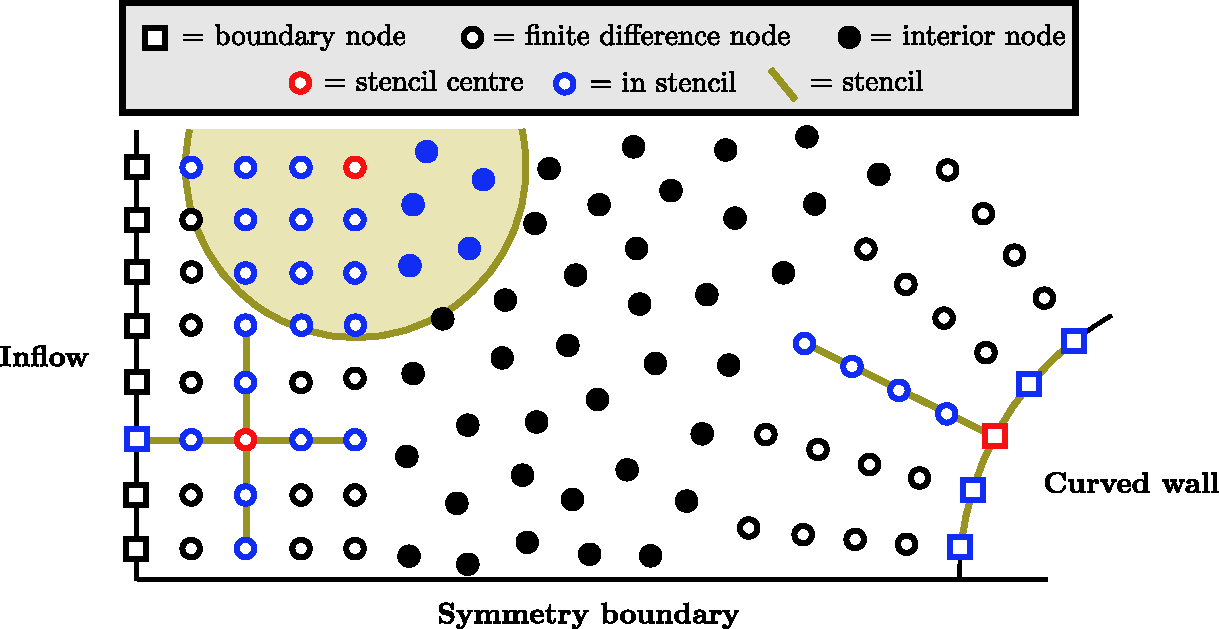
\includegraphics[scale=0.65]{assets/imgs/LABFM-boundary-stencils.pdf}
\vspace*{0.5em}
\caption{Diagram showing a LABFM discretisation of an inflow and curved wall.}
\label{fig:labfm-boundary}
\end{figure}

Under LABFM, the majority of the computational domain is discretised with an unstructured point cloud. This leaves the boundaries (excluding periodic and symmetry boundaries) which are instead discretised using uniformly spaced boundary nodes alongside four more nodes which are evenly spaced normal to the boundary \cite{king2022HighOrderSimulationsIsothermal}. The normal nodes allow normal gradients to be calculated using one-sided (boundary and first row) and centred (third row) finite differences -- these nodes are hence referred to as finite difference nodes. Tangential gradients are calculated via a transformed one-dimensional LABFM on the row of finite difference nodes tangential to the boundary. For the third and fourth row of finite difference nodes, derivatives are simply calculated using lower, usually fourth-order, LABFM. \fig{fig:labfm-boundary} shows these discretisations in a model domain containing a curved wall near an inflow. Importantly, these finite difference nodes can be very efficiently placed into the domain provided the curved boundaries are smooth enough. The rest of the interior point cloud or unstructured nodes are placed after based on an energy minimisation approach \cite{king2020HighOrderDifference}.





\section{Navier-Stokes Characteristic Boundary Conditions} \label{sec:NSCBC}
\sectionmark{NSCBC}

Alongside spatial discretisation, boundary conditions comprise one of the most important parts of any simulation code. Not least because of the modelling which is enforced, but also because of changes to a simulation code's architecture which are necessitated as a result. The NSCBC \cite{poinsot1992BoundaryConditionsDirect,poinsot2001TheoreticalNumericalCombustion} formulation represents not a specific type of boundary condition, but a sort of instruction set to be applied to whichever boundary it concerns. The method was first outlined in \cite{thompson1987TimeDependentBoundary,thompson1987LecturesSeriesComputational,thompson1990TimeDependentBoundaryConditions} for non-reacting one-dimensional flows, in what is now known as the \emph{Locally One-Dimensional Inviscid} (LODI) approximation. The NSCBC formulation was developed as an extension of this to higher-dimensional, reacting flows of imperfect gases, where diffusive effects are included in extra physical conditions on top of those prescribed in the LODI case.


\subsection{The Locally One-Dimensional Inviscid Approximation} \label{sec:LODI}

Any hyperbolic system can be written in the form:
\begin{equation} \label{eqn:hyp-source}
\pdv{\und{U}}{t} + \vnab \cdot\und{\vb{F}} + \und{B} = 0,
\end{equation}
where $\und{U}$ are the $N_\rm{V}$ conservative variables, $\und{\vb{F}}$ are the fluxes for each of these variables in each dimension and $\und{B}$ are source terms. We assume that these terms are non-diffusive for this approximation. Bold variables represent vectors in space, as usual, with their components determined by superscript indices like $F^x$ being the $x$-component of $\vb{F}$. Vectors and matrices of variables, however, are underlined once and twice, respectively, with the intention of providing more clarity. This equation is unique up to linear combinations of the conserved variables, but can be transformed into a form for the primitive variables $\und{V}$:
\begin{equation}
\pdv{\und{V}}{t} + \undt{\vb{A}} \cdot \vnab  \und{V} + \und{b} = 0
\end{equation}
where
\begin{equation}
P_{ij} \equiv \pdv{U_i}{u_j},
\quad
\boldsymbol{Φ}_{ij} \equiv \pdv{\vb{F}_i}{u_j},
\quad
\undt{\vb{A}} \equiv \undt{P}^{-1}\undt{\boldsymbol{Φ}}
\quad \text{and} \quad
\und{b} \equiv \undt{{P}}^{-1}\und{B}.
\end{equation}
The matrix $\undt{P}$ is the Jacobian matrix, $\undt{\vb{A}}$ represents the convection of the variables due to the other variables and themselves (e.g. resulting in $(\vb{u} \cdot \vnab )\vb{u}$ in the momentum equation) and $\und{b}$ are source terms acting on primitive variables. Using this form, we can isolate the $x$-derivatives to observe the characteristics in that direction:
\begin{equation} \label{eqn:with_A}
\pdv{\und{V}}{t} + \undt{A}^x \pdv{\und{V}}{x} + \und{c} = 0
\quad \text{where, in 3D} \quad
\und{c} \equiv \und{b} + \undt{A}^y \pdv{\und{V}}{y} + \undt{A}^z \pdv{\und{V}}{z}
\quad \text{and} \quad
\und{C} \equiv \undt{P} \, \und{c}.
\end{equation}
The statement that the system is hyperbolic is now the statement that the $N_\rm{V}$ eigenvalues $λ_m = λ_m(\und{V})$ of $\undt{A}^x$ are real and can be ordered like $λ_1 \leq \dots \leq λ_{N_\rm{V}}$. Owing to this, we consider the left-eigenvectors $\und{l}_m = \und{l}_m(\und{V})$ of $\undt{A}^x$:
\begin{equation}
\und{l}_m^T \undt{A}^x = λ_m \und{l}_m^T.
\end{equation}
Multiplying equation \equ{eqn:with_A} by an eigenvector we project our equation into a solution space containing only the $m$\sus{th} characteristic invariant, $J_m$, which satisfies $\dd{J_m} = \und{l}_m^T \dd{\und{V}} + \und{l}_m^T \und{c} \dd{t}$ as in \cite{thompson1987LecturesSeriesComputational,thompson1987TimeDependentBoundary}:
\begin{boxequ} \label{eqn:single_char_prob}
\und{l}_m^T \pdv{\und{V}}{t} + λ_m \und{l}_m^T \pdv{\und{V}}{x} + \und{l}_m^T \und{c} = 0,
\quad \iff \quad
\pdv{J_m}{t} + λ_m \pdv{J_m}{x} = 0.
\end{boxequ}
We notice that along any trajectory $\vb{x}_m(t)$ which satisfies $\dd{\vb{x}_m}/\dd{t} = λ_m$ (i.e. the m\sus{th} characteristic has velocity $λ_m$), the invariant obeys:
\begin{equation}
\dv{J_m}{t} = 0.
\end{equation}
This tells us the $J_m$ are constant along the trajectories $\vb{x}_m(t)$, which completes the characteristic analysis traditionally. But, numerically $J_m$ is not so useful since it needs to be transformed back into the primitive variables anyway for a simulation. Instead we use the form of the equation in primitive or conservative variables under the transformation $\undt{A}^x = \undt{S} \, \undt{Λ} \, \undt{S}^{-1}$ where $\undt{Λ}=\rm{diag}(λ_1, \dots, λ_{N_\rm{V}})$ is the diagonal matrix of eigenvalues and rows of the matrix $\undt{S}^{-1}$ are the corresponding \emph{left eigenvectors} $\und{l}_m^T$:
\begin{gather}
\cl{L}_m \equiv λ_m \pdv{J_m}{x} \equiv λ_m \und{l}_m^T \pdv{\und{V}}{x}, \\
\implies \quad
\boxed{
\pdv{\und{V}}{t} + \undt{S} \, \und{\cl{L}} + \und{c} = 0
\quad \text{and} \quad
\pdv{\und{U}}{t} + \undt{P} \, \undt{S} \, \und{\cl{L}} + \und{C} = 0,
}
\label{eqn:char-bcs-end}
\end{gather}
where $\und{\cl{L}} = (\cl{L}_1, \dots, \cl{L}_{N_\rm{V}})$. So each value $\cl{L}_m$ then represents the convection of the m\sus{th} characteristic wave at a point in space. The \emph{Locally One-Dimensional Inviscid} (LODI) characteristic boundary formulation\footnote{So-called as we preclude diffusive effects in any hyperbolic system of equations and we only observe characteristic waves moving over a boundary normal to a single dimension, i.e. not at a corner.} focuses on points at the boundary of a computational domain, and posits that outgoing characteristics through this boundary can be calculated as normal using one-sided derivatives -- which are innately upwinded -- but characteristics entering the domain, such as an acoustic reflection, must instead be modelled. The key to LODI then, is that these incoming waves may be controlled by imposing their respective values of $\cl{L}_m$ at that boundary.

Note that, because we have the matrix $\undt{S}^{-1}$ not $\undt{S}$, we find the flux term $\und{d} \equiv \undt{S} \, \und{\cl{L}}$ by solving the linear system:
\begin{equation}
\undt{S}^{-1} \und{d} = \und{\cl{L}}.
\end{equation}




\subsection{Application to Perfect Reacting Gases}

\begin{figure}[t]
\centering
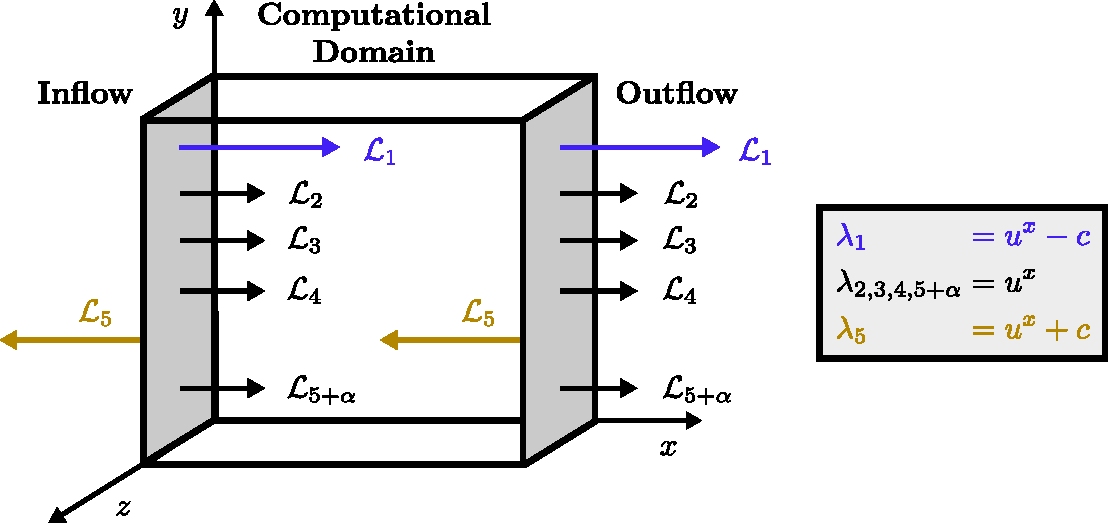
\includegraphics[scale=0.65]{assets/imgs/NSCBC-L.pdf}
\caption{Diagram of $\cl{L}_m$ values for a three-dimensional computational domain simulating a reacting flow. The direction and colour of arrows signifies the direction and strength of the corresponding wave speed $λ_m$.}
\label{fig:NSCBC}
\end{figure}

The LODI approximation of the governing equations of perfect, reacting gases first requires the form of their hyperbolic (non-diffusive) conservation equations. These are:
\begin{subequations}
\begin{alignat}{3}
\pdv{ρ}{t} &+ \vnab  \cdot (ρ \vb{u}) && &&= 0 \\
\pdv{ρ \vb{u}}{t} &+ \vnab  \cdot (ρ \vb{u}\otimes \vb{u} + p I) && - ρ \vb{g} &&= 0 \\
\pdv{ρ e}{t} &+ \vnab  \cdot [(ρ e + p) \vb{u}] && - ρ \vb{g} \cdot \vb{u} &&= 0 \\
\pdv{ρ Y_α}{t} &+ \vnab  \cdot [ρ Y_α \vb{u}] && - \dot{ω}_α &&= 0
\end{alignat}
\end{subequations}
for $α = 1, \dots, N_{\rm{S}}$. The energy $e$ modelled here is the \emph{internal energy of a perfect gas} rather than the total energy specified in \chap{ch:combust-model}. The algebraic equations for internal energy and pressure are, in three-dimensions:
\begin{equation}
ρ e = ρ E_{\rm{th}} + ρ E_{\rm{ki}},
\quad \text{where} \quad
ρ E_{\rm{th}} = \frac{p}{\gamma - 1}
\quad \text{and} \quad
ρ E_{\rm{ki}} = \frac{1}{2} ρ \vb{u} \cdot \vb{u}.
\end{equation}
In this case, the vectors of conservative variables, fluxes and source terms are:
\begin{equation}
\und{U} = \begin{pmatrix} ρ \\ ρ u^x \\ ρ u^y \\ ρ u^z \\ ρ e  \\ ρ Y_1 \\ \vdots \end{pmatrix},
\quad
\und{V} = \begin{pmatrix} ρ \\ u^x \\ u^y \\ u^z \\ e \\ Y_1 \\ \vdots \end{pmatrix},
\quad
\und{F}^x = \begin{pmatrix} ρ u^x \\ ρ u^x u^x + p \\ ρ u^x u^y \\ ρ u^x u^z \\ (ρ e + p) u^x \\ ρ Y_1 u^x \\ \vdots \end{pmatrix},
\quad \text{and} \quad
\und{B} = \begin{pmatrix} 0 \\ - ρ g^x \\ - ρ g^y \\ - ρ g^z \\ - ρ \vb{g} \cdot \vb{u} \\ -\dot{ω}_1 \\ \vdots \end{pmatrix}.
\end{equation}
Hence, we evaluate the relevant matrices:
\begin{equation}
\undt{P} = \begin{pmatrix}
1   & 0  & 0 & 0 & 0 & 0 &  \\
u^x & ρ & 0 & 0 & 0 & 0 &  \\
u^y & 0 & ρ & 0 & 0 & 0 & \cdots \\
u^z & 0 & 0 & ρ & 0 & 0 &  \\
\frac{1}{2} \vb{u} \cdot \vb{u} & ρ u^x & ρ u^y & ρ u^z & 1/(γ - 1) & 0 & \\
Y_1 & 0 & 0 & 0 & 0 & ρ & \\
 &  & \vdots &  &  &  & \ddots
\end{pmatrix}
\end{equation}
so
\begin{equation}
\undt{A}^x = \begin{pmatrix}
u^x & ρ & 0 & 0 & 0 & 0 & \\
0 & u^x & 0 & 0 & 1 / ρ & 0 & \\
0 & 0 & u^x & 0 & 0 & 0 & \\
0 & 0 & 0 & u^x & 0 & 0 & \\
0 & γ p & 0 & 0 & u^x & 0 &  \\
0 & 0 & 0 & 0 & 0 & u^x & \\
 &  & \vdots &  &  &  & \ddots
\end{pmatrix}
\quad \text{and} \quad
\und{b} = \begin{pmatrix} 0 \\ -g^x \\ -g^y \\ -g^z \\ 0 \\ -\dot{ω}_1 / ρ \\ \vdots\end{pmatrix}.
\end{equation}
This gives us the full equations in the primitive variables, the full form of which is omitted. Considering the eigenvalue problem of $\undt{A}^x$, we have:
\begin{subequations} \label{eqn:λ_l_L}
\begin{alignat}{5}
λ_1 &= u^x - c  \qquad && \und{l}^T_1 &&= (0, -ρ c, 0, 0, 1, 0, \dots) \quad && \text{and} \quad \cl{L}_1 &&= λ_1 \left(\pdv{p}{x} - ρ c \pdv{u^x}{x}\right), \\
λ_2 &= u^x      \qquad && \und{l}^T_2 &&= (c^2, 0, 0, 0, -1, 0, \dots)  \quad && \text{and} \quad \cl{L}_2 &&= λ_2 \left(c^2 \pdv{ρ}{x} - \pdv{p}{x}\right), \\
λ_3 &= u^x      \qquad && \und{l}^T_3 &&= (0, 0, 1, 0, 0, 0, \dots)     \quad && \text{and} \quad \cl{L}_3 &&= λ_3 \pdv{u^y}{x}, \\
λ_4 &= u^x      \qquad && \und{l}^T_4 &&= (0, 0, 0, 1, 0, 0, \dots)     \quad && \text{and} \quad \cl{L}_4 &&= λ_4 \pdv{u^z}{x}, \\
λ_5 &= u^x + c  \qquad && \und{l}^T_5 &&= (0, ρ c, 0, 0, 1, 0, \dots)     \quad && \text{and} \quad \cl{L}_5 &&= λ_5 \left(\pdv{p}{x} + ρ c \pdv{u^x}{x}\right), \\
λ_{5 + 1} &= u^x      \qquad && \und{l}^T_{5 + 1} &&= (0, 0, 0, 0, 0, 1, \dots)     \quad && \text{and} \quad \cl{L}_{5 + 1} &&= λ_{5 + 1} \pdv{Y_1}{x}
\end{alignat}
\end{subequations}
and so on. For the inverse problem:
\begin{subequations}
\begin{alignat}{5}
& \pdv{ρ}{x}   &&= \frac{1}{c^2} \left[ \frac{\cl{L}_2}{λ_2} + \frac{1}{2} \left( \frac{\cl{L}_5}{λ_5} + \frac{\cl{L}_1}{λ_1} \right) \right] && \quad \text{and} \quad && d_1 &&= \frac{1}{c^2}\left[\cl{L}_2 + \frac{1}{2} \left( \cl{L}_5 + \cl{L}_1 \right) \right], \\
& \pdv{u^x}{x} &&= \frac{1}{2 ρ c}\left(\frac{\cl{L}_5}{λ_5} - \frac{\cl{L}_1}{λ_1}\right) && \quad \text{and} \quad && d_2 &&= \frac{1}{2 ρ c}(\cl{L}_5 - \cl{L}_1), \\
& \pdv{u^y}{x} &&= \frac{\cl{L}_3}{λ_3} && \quad \text{and} \quad && d_3 &&= \cl{L}_3, \\
& \pdv{u^z}{x} &&= \frac{\cl{L}_4}{λ_4} && \quad \text{and} \quad && d_4 &&= \cl{L}_4, \\
& \pdv{p}{x}   &&= \frac{1}{2}\left(\frac{\cl{L}_5}{λ_5} + \frac{\cl{L}_1}{λ_1}\right) && \quad \text{and} \quad && d_5 &&= \frac{1}{2}(\cl{L}_5 + \cl{L}_1), \\
& \pdv{Y_1}{x} &&= \frac{\cl{L}_{5 + 1}}{λ_{5 + 1}} && \quad \text{and} \quad && d_{5 + 1} &&= \cl{L}_{5 + 1}
\end{alignat}
\end{subequations}
and so on. Evidently, the eigenvalues $λ_1$ and $λ_5$ correspond to the speed of sound but since positive $x$ points into the domain, only one of these corresponds to an acoustic wave entering the domain.


\subsection{Non-Reflecting Subsonic Boundaries}

\subsubsection{Outflows}

The first non-reflective boundaries under this formulation come from \cite{thompson1987TimeDependentBoundary} in the case of the one-dimensional, subsonic, inviscid, non-isothermal Euler equations (the equations above if we lower the dimension of $\vb{x}$ and $\vb{u}$ and drop the mass fraction equations). This was promptly extended to the set of equations shown above in \cite{poinsot1992BoundaryConditionsDirect} for reacting flows. In both cases, a simple condition for acoustically non-reflecting boundaries was found by requiring that the Riemann invariant corresponding to the entering acoustic wave remain constant under the assumption that transverse terms can be neglected. At a subsonic outflow boundary on the left end of the computational domain, where $0 < u^x < c$, this means the invariant $J_5$ should remain constant at the boundary, provided transverse derivatives vanish. Equivalently, we require
\begin{equation}
0 = \und{l}^T_5 \pdv{\und{V}}{t} = \left( \pdv{p}{t} + ρ c \pdv{u^x}{t} \right)
\end{equation}
given that, from equation \equ{eqn:single_char_prob}:
\begin{equation}
0 = \und{l}^T_5 \pdv{\und{V}}{t} + \cl{L}_5 + \und{l}^T_5 \und{b} = \left( \pdv{p}{t} + ρ c \pdv{u^x}{t} \right) + \cl{L}_5 - ρ c g^x.
\end{equation}
So we must enforce $\cl{L}_5 = ρ c g^x$. Similarly, a subsonic outflow at the right end of the computational domain requires $\cl{L}_1 = - ρ c g^x$.

\subsubsection{Inflows}

For subsonic outflows, regardless which side of the domain they reside, the only characteristic wave which enters the domain are either $\cl{L}_5$ for left-side boundaries and $\cl{L}_1$ for right-side boundaries, as shown in \fig{fig:NSCBC}. All the other $\cl{L}_m$ values required in \equ{eqn:char-bcs-end} may be found via the one-sided derivatives mentioned above. For inflows the situation flips on its head. We instead have access to \emph{only} $\cl{L}_1$ for left-side boundaries and $\cl{L}_5$ for right-side boundaries and all others represent waves which must be modelled as we have no information on in the interior and boundary of the domain. Presuming our inflow is on the left end of the computational domain, then $\cl{L}_1$ may be found from the interior, as above, $\cl{L}_5$ may be found using the acoustic non-reflection condition for the outflows, also as above, and the rest must model some sensible physics on waves entering the domain. For example, the entrance of shear waves into the domain are given by $\cl{L}_{3}$ and $\cl{L}_{4}$, but may be removed simply by assigning $\cl{L}_{3} = g^y$ and $\cl{L}_{4} = g^z$. The entropy and species density waves $\cl{L}_{2}$ and $\cl{L}_{5 + α}$ are assigned zero as the corresponding source terms in $\und{b}$ vanish.


\subsection{Extra Boundary Considerations}

For wall boundaries, the SUNSET code uses the NSCBC formulation described above to implement adiabatic walls by reflecting entropy waves and isothermal walls by \emph{not} reflecting entropy waves. On inflows and outflows, according to \cite{sutherland2003ImprovedBoundaryConditions} the SUNSET code uses the diffusive BCs given by \equ{eqn:znf}, the zero normal flux conditions. As suggested by \cite{sutherland2003ImprovedBoundaryConditions} and \cite{yoo2007CharacteristicBoundaryConditions}, source and transverse terms are included into the characteristic boundaries so shear phenomena can effectively pass through these boundaries. Although, for the BCs outlined in the next section, they will not be used. The same can be said about relaxation terms for inflows and outflows, which are typically used to ensure well-posedness and remove variable drift, as they are not needed in the upcoming BCs.


\cleardoublepage

\chapter{Acoustic Delay Characteristic Boundary Conditions} \label{ch:delay-bcs}
\chaptermark{ADCBC}
\section{Delayed Acoustics Model}

Investigating the physics of of a thermoacoustic interaction requires the resolving of the full non-linear acoustics in the combustion system -- this might typically be a plenum, inlet, combustor and exhaust -- as well as the highly local reaction and diffusion phenomena located at the flame. In the case of a deflagration in a tube, the acoustics span the whole tube and a premixed flame and surrounding hydrodynamics will be located in one relatively small region of this tube. It would be natural, then, to fully resolve the flame and hydrodynamics by a fully simulated region and leave the which are the dominant effect upstream and downstream of the flame to be modelled separately. Assume at the simulation inflow that we can decompose the pressure and velocity fields, $\vb{u}=(u, v)$ in two-dimensions, as $u = \overline{u} + u_a$ and $p = \overline{p} + p_a$, where $\overline{\cdot}$ represents the non-acoustic field at the inflow and $\cdot_a$ represents acoustic fluctuations. Then the value of $\overline{u} \pm c$ determines the speed of acoustic waves through the tube. Under a linear assumption for these acoustics -- i.e. the assumption that $ρ \approx \overline{ρ}$ such that $\abs{ρ_a} \ll 1$ or equivalently that acoustics do not interact with each other -- then the convection of an acoustic wave in a headwind and tailwind will cancel out. This results in a representative time delay $τ$ for the acoustic wave to leave the simulation domain, travel a distance $l$ both ways up- or downstream, and reenter:
\begin{equation}
τ = \frac{l}{c + u} + \frac{l}{c - u} = \frac{2l}{c} \, \frac{1}{1 - \Ma} \approx \frac{2l}{c}
\end{equation}
since under the deflagration approximation $\Ma \ll 1$. This is the time delay we will associate with the simulation inflow and outflow to represent their length scale via the delayed reentry of these acoustic into the inflow and outflow after a delay $τ_{\rm{U}}$ and $τ_{\rm{D}}$ respectively. This solves the linear acoustic problem in the tube upstream and downstream of the flame to leading order in Mach number. We refer to this non-DNS domain by the acoustic or fictitious domain or region.

\begin{figure}[t]
\centering
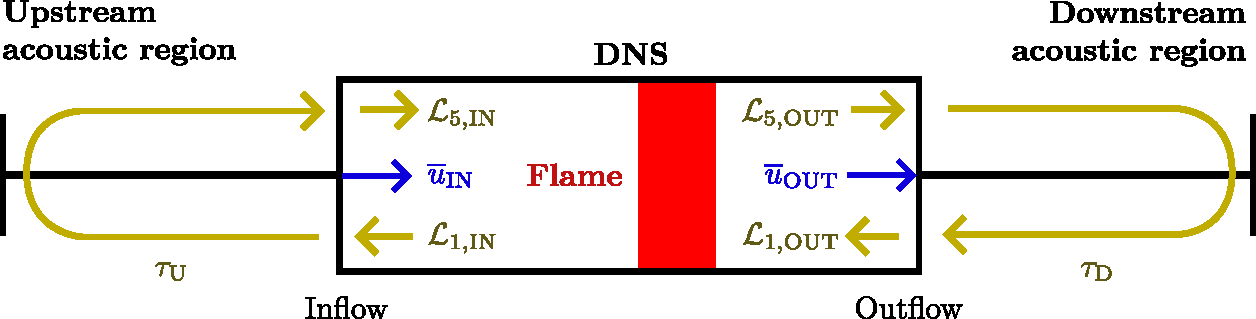
\includegraphics[scale=0.65]{assets/imgs/delay_bc_model.pdf}
\caption{Simple diagram for the simulation model.}
\label{fig:delay-model}
\end{figure}

To fit this model into the existing characteristic boundary formulation provided by NSCBC and LODI, we assume that we can store all of the outgoing acoustics as $\cl{L}_{\text{outgoing acoustic}}(t, \vb{y})$ where $\vb{y}$ parameterises the given connected inflow or outflow (this is a scalar value $y$ for 2 dimensional problems with vertical inflow or outflow). For a rectangular two-dimensional horizontal tube, this becomes $\cl{L}_{1/5}(t, y)$ where the outgoing acoustic is $\cl{L}_{1}$ for left-side boundaries and $\cl{L}_{5}$ for right-side boundaries (inflows and outflows respectively in this report). A simple diagram of the acoustic behaviour is shown in \fig{fig:delay-model} as acoustic values leave and reenter the DNS domain repeatedly. Continuing with this two-dimensional example, we would impose the delayed acoustic reentry by imposing at the left-side boundary that:
\begin{subequations}
\begin{equation}
\cl{L}_{5, \rm{IN}}(t, y) = \cl{L}_{5, \rm{IN}, \rm{nonreflect}}(t, y) + R_{\rm{U}} \cl{L}_{1, \rm{IN}}(t - τ, y),
\end{equation}
and at the right-side boundary:
\begin{equation}
\cl{L}_{1, \rm{OUT}}(t, y) = \cl{L}_{1, \rm{OUT}, \rm{nonreflect}}(t, y) + R_{\rm{D}} \cl{L}_{5, \rm{OUT}}(t - τ, y)
\end{equation}
\end{subequations}
where $R_{\rm{U/D}}$ are the reflection coefficients at the up- and downstream acoustic boundaries. For a closed tube this would be $R = 1$ and for an open tube $R = -1$. The first term $\cl{L}_{\dots,\: \rm{nonreflect}}$ is the required condition described in the previous chapter to stop the outgoing acoustic from being immediately reflected. Under this model, we are implicitly assuming each location at the boundary has its own one-dimensional acoustic approximation being made. For the rest of the report we instead use a simpler formulation which averages the acoustics across the boundary as they leave:
\begin{subequations}
\begin{equation} \label{eqn:L-delay-form}
\cl{L}_{5, \rm{IN}}(t, y) = \cl{L}_{5, \rm{IN}, \rm{nonreflect}}(t, y) + R_{\rm{U}} \langle \cl{L}_{1, \rm{IN}}(t - τ_{\rm{U}}, \cdot\,) \rangle_{\rm{IN}}
\end{equation}
for inflows and:
\begin{equation}
\cl{L}_{1, \rm{OUT}}(t, y) = \cl{L}_{1, \rm{OUT}, \rm{nonreflect}}(t, y) + R_{\rm{D}} \langle \cl{L}_{5, \rm{OUT}}(t - τ_{\rm{D}}, \cdot\,) \rangle_{\rm{OUT}}
\end{equation}
\end{subequations}
%(NOT SURE WHAT TO DO IF THESE WAVES DO NOT FULLY REFLECT?)
for outflows. The operator $\langle\,\cdot\,\rangle_{\rm{IN/OUT}}$ represents averaging over inflow or outflow boundary values respectively. To simplify notation, we write $\overline{\cl{L}}_{\rm{IN/OUT}}(t') \equiv \langle \cl{L}_{1/5, \rm{IN/OUT}}(t', \cdot\,) \rangle_{\rm{IN/OUT}}$ from now on. This corresponds to a single one-dimensional approximation being made for each boundary, which is of course only valid for thin-enough computational domains.

Since we are modelling the reaction Navier-Stokes equations, we must also impose that all other incoming $\cl{L}$ values vanish at the inflow so that no entropy, shear or mass waves enter the domain. Note that now no relaxation terms are used on either boundary -- this marks the main difference between ADCBC and NSCBC. Relaxation terms are traditionally used under the NSCBC formulation to ensure the dependent variables -- inflow velocities, temperature or density and mass fractions and especially outflow pressure -- do not drift as characteristic waves leave the domain, not to return under perfectly non-reflecting conditions. Given that the acoustic waves will be returning under ADCBC, we do not need these relaxation terms for inflow normal velocity ($u$ in our vertical boundaries) or outflow pressure as they are closed by the full reflection of these acoustic waves. Note that if relaxation terms were imposed on top of the delayed reflections, we would be applying a further well-posing condition to a problem which is already well-posed. Note that we must have $\abs{R} = 1$ since we do not yet know how to deal with the resulting pressure drift when $\abs{R} < 1$ without using these relaxation terms. For the other variables, relaxation terms may be kept, but we have chosen to remove them under the assumption that the simulation is strongly one-dimensional and inert at the boundary. That is, no significant shear, entropy or mass waves should be leaving these boundaries, so the related dependent variables $v$, $T$, $Y_α$ will not drift. All that is left is to apply the diffusive BCs as the remaining physical BCs. Nothing here changes with \cite{sutherland2003ImprovedBoundaryConditions}, where they use the zero normal flux conditions \equ{eqn:znf}. A further consideration to make is what happens when the acoustic field is strong enough that $\abs{\overline{u}} < \abs{u_a}$ at the inflow or outflow. Usually we expect this to happen at the inflow first since $\abs{\overline{u}_{\rm{IN}}} > \abs{\overline{u}_{\rm{OUT}}}$, i.e. the acoustic field has become large enough that the inflow has become an outflow at the left side of the domain. To account for this, we simply check if the sign of $\vb{u}\cdot\uvec{n}$ at this boundary where $\uvec{n}$ is the outward pointing normal and apply the conditions for $\cl{L}_m$ and diffusion correspondingly.

To outline the method once more, we will be introducing a delay for acoustics leaving the simulation domain to model an extended acoustic domain which is not a part of this acoustic region. This will be done using non-reflecting characteristic boundaries and storing the acoustics which leave the domain. These acoustics are then simply reintroduced after the relevant time delay. We refer to these boundary conditions as \emph{Acoustic Delay Characteristic Boundary Conditions} (ADCBC).

Later on, these definitions for $\cl{L}_{1/5}$ can be extended to include an imposed acoustic field if that is desirable, e.g. to simulate a secondary thermoacoustic instability response. Furthermore, this method could also be extended to arbitrary numbers of delay boundaries with any boundary normal, although modelling a physical geometry in this way would be a challenge which is not explored in this work.




\section{Implementing the Model}

%% THIS ALSO MEANS WE MUST DISCRETISE THE INTEGRALS FOR FIELD RECONSTRUCTION

The SUNSET code, like other CFD codes, uses a discretised temporal domain to integrate forward in time. Hence, we already only have access to the outgoing characteristics at discrete time steps and cannot recover the exact value of $\overline{\cl{L}}_{\rm{IN/OUT}}(t - τ)$ when $t - τ$ does not lie on a previous time step. Omit subscripting for now for brevity. On top of this, the step size taken by a typical combustion simulation is likely to oversample the acoustic field at the boundary, resulting in a much higher memory footprint that is required by the method. This, along with the variable time steps used in the SUNSET code means we aim for a sample rate $δt_{\rm{sample}} > δt > 0$ for these $\overline{\cl{L}}$ values. We refer to the sample times and acoustics as $\{(t_s, \overline{\cl{L}}_{s})\}_{s=1}^{N_{\rm{samp}}}$ where $s\in\bb{Z}$ enumerates these sample times so $t_{N_{\rm{samp}}}$ is the most recent sample time and $\overline{\cl{L}}_{s} \equiv \overline{\cl{L}}(t_s)$. To evaluate the $\overline{\cl{L}}(t - τ)$ term on the right-hand side of \equ{eqn:L-delay-form}, we simply interpolate between values of $(t_s, \overline{\cl{L}}_{s})$ at the interpolated time $t' \equiv t - τ$. Note that no requirement is made here that this interpolation conserve the acoustic energy which left the domain. If significant acoustic losses or gains are made as a result of this, an acoustically conservative method should later be investigated.


\subsection{Code Schematic}

Since the time delay is only a finite length, clearly the oldest sample values we require are $\overline{\cl{L}}(t')$ where $t' \approx t - τ - δt_{\rm{sample}}$. Hence, we only need to store the finite number of samples $\bb{T} \cross \bb{L} = \{(t_s, \overline{\cl{L}}_{s}) \, : \, t_s \in [t - τ - δt_{\rm{sample}}, t]\}_{s=1}^{N_{\rm{samp}}}$ at any given simulation time $t$. For as long as $τ$ remains bounded, the size of $\bb{T} \cross \bb{L}$ -- and hence our memory footprint -- also remains bounded. Thus far, we have assumed that the up- and downstream tube lengths $l_{\rm{U/D}}$ remain constant, but they may actually change arbitrarily alongside their associated time delays $τ_{\rm{U/D}}$ provided it does not exceed the sound speed, so multiple acoustics do not reenter the domain at one sample time. Having said that, as long as we know the maximum delay time $τ$ occurring in a given simulation, we can store $\bb{T} \cross \bb{L}$ in a contiguous portion of memory which the delay boundaries are allocated at the beginning of the simulation. This is done using a one-sided queue data structure, which is implemented as a \emph{first-in, first-out} (FIFO) wrapper around a contiguous array. In this way, samples from the current simulation time may be added to the end of the queues and values which are needed for interpolation are found at the beginning of the queue. Once they are no longer needed for an accurate interpolation of $\overline{\cl{L}}(t - τ)$, they are \emph{popped} (removed) from the beginning of the queue. If some other data structure was used instead for these samples, then the data would slink through memory in a way where \emph{contiguity} cannot be enforced for arbitrary simulation times. Note that a linked list would be subject to this issue, be slower to traverse for interpolation values and provide $\cl{O}(1)$ deletion of random samples, which we do not require here.

\begin{figure}[t]
\centering
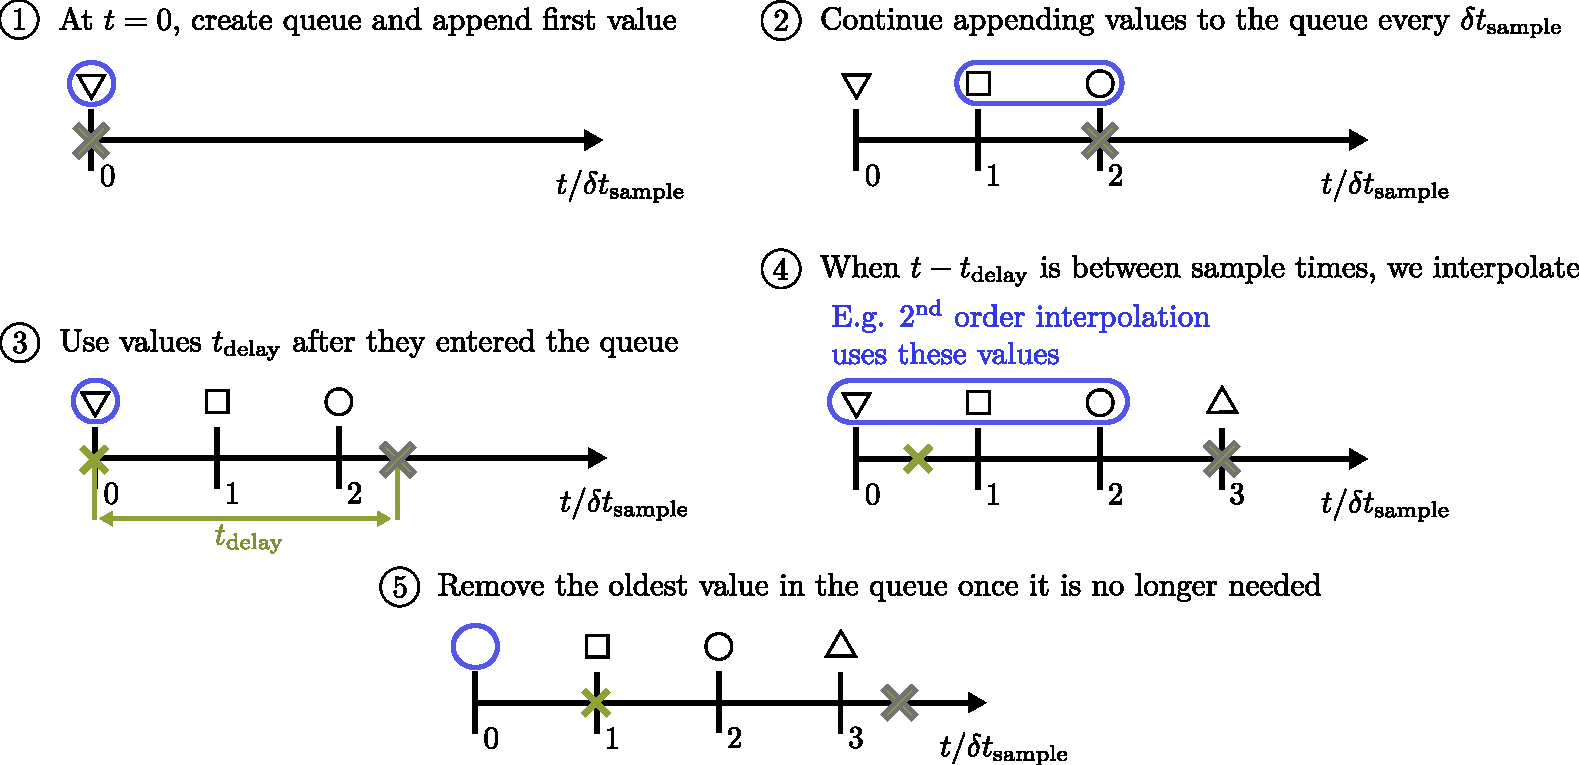
\includegraphics[scale=0.65]{assets/imgs/delay_bc_queue.pdf}
\caption{An illustration of how this queue system is used for boundary sampling. Different shapes are used to represent the different values in $\bb{T} \cross \bb{L}$. The values relevant to the current step is circled in blue.}
\label{fig:delay-queue}
\end{figure}

This queue system is illustrated in \fig{fig:delay-queue} in a continuous temporal domain for simplicity so sample times remain uniformly spaced. The first two steps, (1) and (2) show values being appended to the queue at the beginning of the simulation until the time delay is reached in the third step, (3). The fourth step, (4) shows which values are used for interpolation in an example second order interpolant. The fifth and final step, (5) shows old values being removed from the start of the queue.

\begin{figure}[t]
\centering
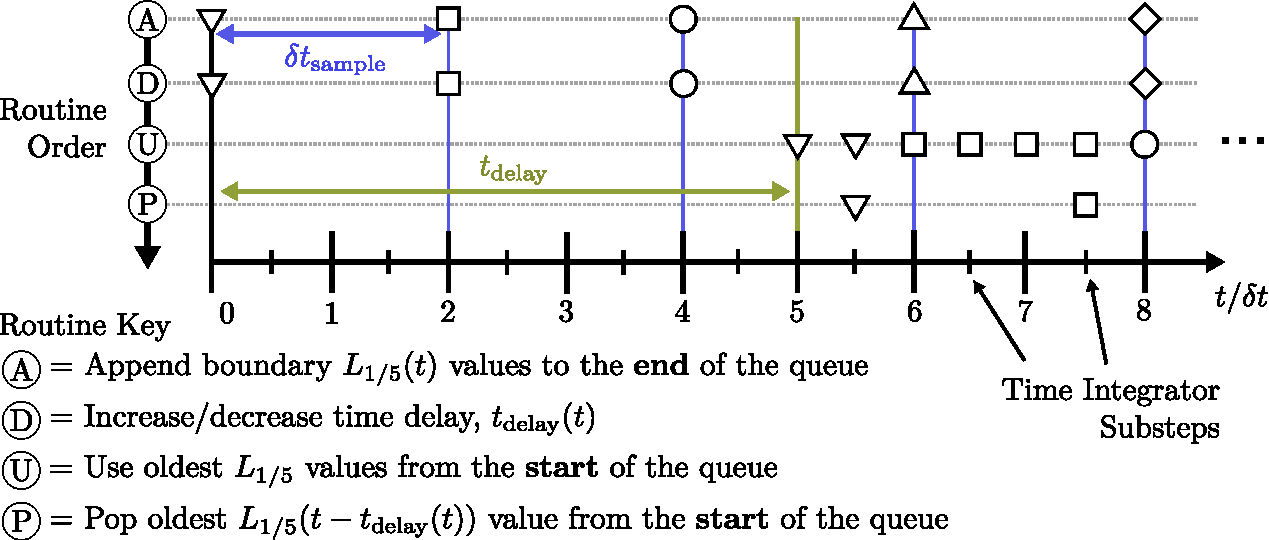
\includegraphics[scale=0.65]{assets/imgs/delay_bc_code_schematic.pdf}
\caption{Routine schematic for ADCBC implemented into a time integrator with two substeps. A sample period $δt_{\rm{sample}} = 2δt$ is used in this example. The evaluation of routines (or procedures) are shown in order from top to bottom (starting with (D) and ending with (U), key given in the figure), left to right (beginning at $t = 0$ and showing up to $t = 8 δt$). A routine being used is signified by a shape representing given sample in $\bb{T} \cross \bb{L}$. The time delay $τ \approx 4 \frac{3}{4} δt$ is shown in gold.}
\label{fig:schematic}
\end{figure}

\fig{fig:schematic} illustrates the full schematic for a time integrator with two substeps per time step and uniform time step size. Sampling is performed in the routine (A) which is called every sample time preceded by a change to $τ$, if required. These are circled and labelled (1) and (2) corresponding to the steps in \fig{fig:delay-queue}. Only after the full time delay $τ$ do the values from the beginning of the queue start to get used in the routine (U). This is shown in the labels (3) and (4) corresponding to those steps in \fig{fig:delay-queue}. Finally, step (5) removes the oldest value from the queue only once they are not needed in the routine (R). Appending and removal from the queue happen before the queue values are used for interpolation to ensure the correct values are available in the queue for interpolation. Note that the routine (U) happens every substep using as many values from the beginning of the queue as are required. The shape shown for this routine in steps (3) and (4) are just the earliest sample taken which would be used.



\subsection{Memory Footprint}

The obvious disadvantage of this ADCBC method is the potential size of queues required to hold the data in $\bb{T} \cross \bb{L}$. This data should only be available to those processors relevant to the boundary nodes, so the memory burden should be held by those processors alone, since the SUNSET code is ran as a distributed system, where memory is allocated to each processor separately. If the memory footprint is too large (on the order of one gigabyte for modern hardware), then the simulations will likely crash and high-memory compute nodes would be required. This is to be avoided. Let us now perform a simple calculation to estimate the memory required by a given acoustic delay characteristic boundary. Assume $l = 1$ m, $c = 343$ m s$^{-1}$ and that a typical sample period is approximately $δt_{\rm{sample}} = 10^{-7}$ s (this will be validated in the coming chapter). Then, the number of numbers which need to be stored in memory are:
\begin{equation}
N_{\rm{numbers}} = 2 \frac{τ}{δt_{\rm{sample}}}
= \frac{4 \, l}{c \, δt_{\rm{sample}}}
\approx 1.17 \cross 10^5.
\end{equation}
For double precision floating point numbers, these require 8 bytes of storage each, resulting in $9.33 \cross 10^5$ bytes $\approx 1$ MB. This can easily be stored and accessed with modern memory, albeit may not be stored in the boundary processor's cache. Overall, this is not a concern as remaining memory required by the LABFM discretisation dwarfs this.

In a separate formulation where acoustics across the boundary are not averaged and instead we have separate queues for samples taken at each boundary node, we are likely to have less than 100 boundary nodes per processor in two-dimensions (and fewer or the same in three). This results in a 100 MB memory requirement, which is still manageable. If longer, e.g. $l = 10$ m, domains are modelled, then this could become a significant issue. Importantly, the total memory requirement under this method is significantly lower than if you had discretised the fully non-linear acoustics in the up- and downstream regions, but these discretisations would be easier to decompose into separate processors. The potential issue then, comes from the fact that this memory burden is placed only onto the boundary nodes, which would have less memory available than the total memory provided in a theoretical decomposition of the acoustic region between more processors.



\section{Acoustic Region Field Reconstruction}

\begin{figure}[t]
\centering
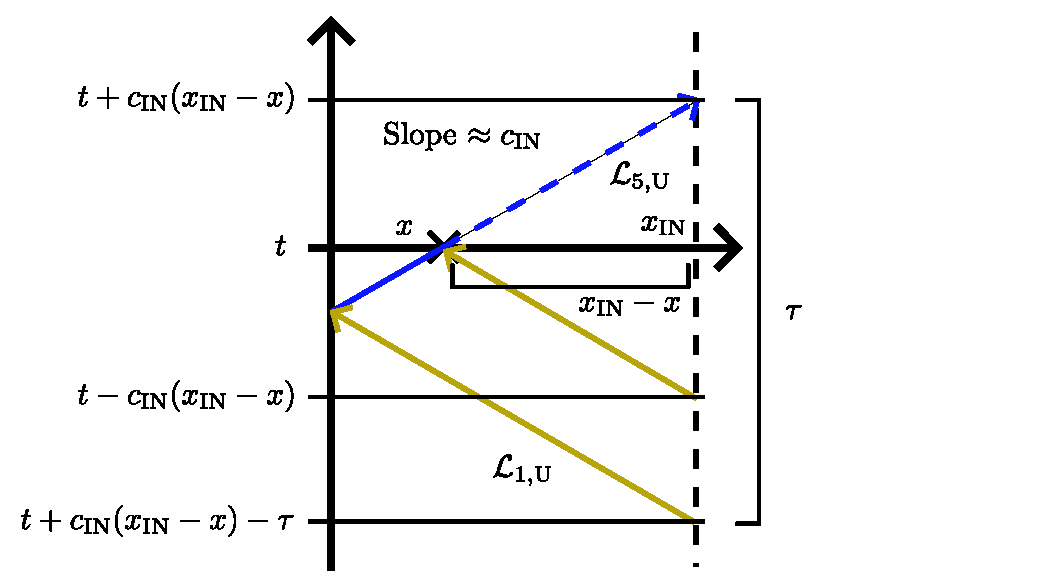
\includegraphics[scale=0.65]{assets/imgs/inlet-adcbc-spatial-field.pdf}
\caption{FIELD RECONSTRUCTION}
\label{fig:field-reconstruction}
\end{figure}

Already having made the low-Mach and linear acoustics approximations makes the reconstruction of acoustic fields in an acoustic region easy as we can approximate the motion of acoustic variables $J_{1/5}$ through the acoustic region as having a constant speed $c$. Hence, we can reinterpret a time series of previous $\overline{\cl{L}}_{\rm{IN/OUT}}(t')$ which leave the ADCBC boundaries as spatial information: the longer ago the acoustic exited through the ADCBC boundary, the farther into its acoustic trajectory it should be. Following the diagram shown in \fig{fig:field-reconstruction}, we have in the upstream region:
\begin{subequations}
\begin{alignat}{2}
\cl{L}_{1, \rm{U}}(t, x) &= &&\overline{\cl{L}}_{\rm{IN}}(t - c_{\rm{IN}}(x_{\rm{IN}} - x))
\quad \text{and} \\
\cl{L}_{5, \rm{U}}(t, x) &= R_{\rm{U}} \, &&\overline{\cl{L}}_{\rm{IN}}(t + c_{\rm{IN}}(x_{\rm{IN}} - x) - τ_{\rm{U}}),
\end{alignat}
and in the downstream region:
\begin{alignat}{2}
\cl{L}_{5, \rm{D}}(t, x) &= &&\overline{\cl{L}}_{\rm{OUT}}(t - c_{\rm{OUT}}(x - x_{\rm{OUT}}))
\quad \text{and} \\
\cl{L}_{1, \rm{D}}(t, x) &= R_{\rm{D}} \, &&\overline{\cl{L}}_{\rm{OUT}}(t + c_{\rm{OUT}}(x - x_{\rm{OUT}}) - τ_{\rm{D}}).
\end{alignat}
\end{subequations}
Using these fields, we can reconstruct the acoustic pressure and velocity by integrating backwards into the upstream region:
\begin{subequations}
\begin{alignat}{2}
p_{a, \rm{U}}(t, x) &= p_{a, \rm{U}}(t, x_{\rm{IN}}) + \frac{1}{2c_{\rm{IN}}} &&\int_{x}^{x_{\rm{IN}}} (\cl{L}_{1, \rm{U}}(t, x') - \cl{L}_{5, \rm{U}}(t, x')) \dd{x'}
\quad \text{and} \\
u_{a, \rm{U}}(t, x) &= u_{a, \rm{U}}(t, x_{\rm{IN}}) + \frac{1}{2c_{\rm{IN}}} \, \frac{1}{ρ_{\rm{IN}} c_{\rm{IN}}} &&\int_{x}^{x_{\rm{IN}}} (\cl{L}_{1, \rm{U}}(t, x') + \cl{L}_{5, \rm{U}}(t, x')) \dd{x'},
\end{alignat}
and forwards into the downstream region:
\begin{alignat}{2}
p_{a, \rm{D}}(t, x) &= p_{a, \rm{D}}(t, x_{\rm{OUT}}) + \frac{1}{2c_{\rm{OUT}}} &&\int_{x_{\rm{OUT}}}^{x} (\cl{L}_{5, \rm{D}}(t, x') - \cl{L}_{1, \rm{D}}(t, x')) \dd{x'}
\quad \text{and} \\
u_{a, \rm{D}}(t, x) &= u_{a, \rm{D}}(t, x_{\rm{OUT}}) + \frac{1}{2c_{\rm{OUT}}} \, \frac{1}{ρ_{\rm{OUT}} c_{\rm{OUT}}} &&\int_{x_{\rm{OUT}}}^{x} (\cl{L}_{1, \rm{D}}(t, x') + \cl{L}_{5, \rm{D}}(t, x')) \dd{x'}.
\end{alignat}
\end{subequations}
Notice that this means the upstream acoustic fields, for example, can be full reconstructed using information only from $t' \in [t - τ, t]$.

To use this continuous derivation on our discrete data, we must discretise the fields onto our samples $\bb{T}\cross\bb{L}$. This means defining the fields in the upstream upstream region as:
\begin{subequations}
\begin{alignat}{3}
\cl{L}_{1, \rm{U}}(t, x) &= &&\overline{\cl{L}}_{\rm{IN}, s_{1, \rm{U}}(t, x)}
\quad && \text{where} \quad
s_{1, \rm{U}}(t, x) \equiv \rm{round}(t - c_{\rm{IN}}(x_{\rm{IN}} - x))
\quad \text{and} \\
\cl{L}_{5, \rm{U}}(t, x) &= R_{\rm{U}} \, &&\overline{\cl{L}}_{\rm{IN}, s_{5, \rm{U}}(t, x)}
\quad && \text{where} \quad
s_{5, \rm{U}}(t, x) \equiv \rm{round}(t + c_{\rm{IN}}(x_{\rm{IN}} - x) - τ_{\rm{U}})
\end{alignat}
where the function round rounds to the nearest integer and in the downstream region:
\begin{alignat}{3}
\cl{L}_{5, \rm{D}}(t, x) &= &&\overline{\cl{L}}_{\rm{OUT}, s_{5, \rm{D}}(t, x)}
\quad && \text{where} \quad
s_{5, \rm{D}}(t, x) \equiv \rm{round}(t - c_{\rm{OUT}}(x - x_{\rm{OUT}}))
\quad \text{and} \\
\cl{L}_{1, \rm{D}}(t, x) &= R_{\rm{D}} \, &&\overline{\cl{L}}_{\rm{OUT}, s_{1, \rm{D}}(t, x)}
\quad && \text{where} \quad
s_{1, \rm{D}}(t, x) \equiv \rm{round}(t + c_{\rm{OUT}}(x - x_{\rm{OUT}}) - τ_{\rm{D}})
\end{alignat}
\end{subequations}
such that the discretised integrals become discrete sums:
\begin{subequations}
\begin{alignat}{2}
p_{a, \rm{U}}(t, x) &= p_{a, \rm{U}}(t, x_{\rm{IN}}) + \frac{1}{2} &&\left( \sum_{s = s_{1, \rm{U}}(t, x)}^{s_{1, \rm{U}}(t, x_{\rm{IN}})} \overline{\cl{L}}_{\rm{IN}, s} - \sum_{s = s_{5, \rm{U}}(t, x)}^{s_{5, \rm{U}}(t, x_{\rm{IN}})} \overline{\cl{L}}_{\rm{IN}, s} \right)δt_{\rm{sample}}
\quad \text{and} \\
u_{a, \rm{U}}(t, x) &= u_{a, \rm{U}}(t, x_{\rm{IN}}) + \frac{1}{2} \, \frac{1}{ρ_{\rm{IN}} c_{\rm{IN}}} &&\left( \sum_{s = s_{1, \rm{U}}(t, x)}^{s_{1, \rm{U}}(t, x_{\rm{IN}})} \overline{\cl{L}}_{\rm{IN}, s} + \sum_{s = s_{5, \rm{U}}(t, x)}^{s_{5, \rm{U}}(t, x_{\rm{IN}})} \overline{\cl{L}}_{\rm{IN}, s} \right) δt_{\rm{sample}}
\end{alignat}
and forwards into the downstream region:
\begin{alignat}{2}
p_{a, \rm{D}}(t, x) &= p_{a, \rm{D}}(t, x_{\rm{OUT}}) + \frac{1}{2} &&\left( \sum_{s = s_{5, \rm{D}}(t, x_{\rm{OUT}})}^{s_{5, \rm{D}}(t, x)} \overline{\cl{L}}_{\rm{OUT}, s} - \sum_{s = s_{1, \rm{D}}(t, x_{\rm{OUT}})}^{s_{1, \rm{D}}(t, x)} \overline{\cl{L}}_{\rm{OUT}, s} \right) δt_{\rm{sample}}
\quad \text{and} \\
u_{a, \rm{D}}(t, x) &= u_{a, \rm{D}}(t, x_{\rm{OUT}}) + \frac{1}{2} \, \frac{1}{ρ_{\rm{OUT}} c_{\rm{OUT}}} &&\left( \sum_{s = s_{1, \rm{D}}(t, x_{\rm{OUT}})}^{s_{1, \rm{D}}(t, x)} \overline{\cl{L}}_{\rm{OUT}, s} + \sum_{s = s_{5, \rm{D}}(t, x_{\rm{OUT}})}^{s_{5, \rm{D}}(t, x)} \overline{\cl{L}}_{\rm{OUT}, s} \right) δt_{\rm{sample}}
\end{alignat}
\end{subequations}
under the assumption that samples are equally space out such that $t_{s} - t_{s - 1} = δt_{\rm{sample}}$. For real simulation data from the SUNSET code variable time steps are used, so this assumption is impossible to enforce, which will introduce some error into the acoustic field reconstruction. Alternatively, we simply replace the sample spacing $δt_{\rm{sample}}$ by $t_{s} - t_{s - 1}$ in the sums above. In either case, these can be calculated from the sampled queue values $\bb{T}\cross\bb{L}$, which can be output from the SUNSET code at arbitrary times we want to observe the acoustic field. These fields can then be viewed using the above formulae as a post-processing step.




\section{Sampling Error}

\begin{figure}[t]
\centering
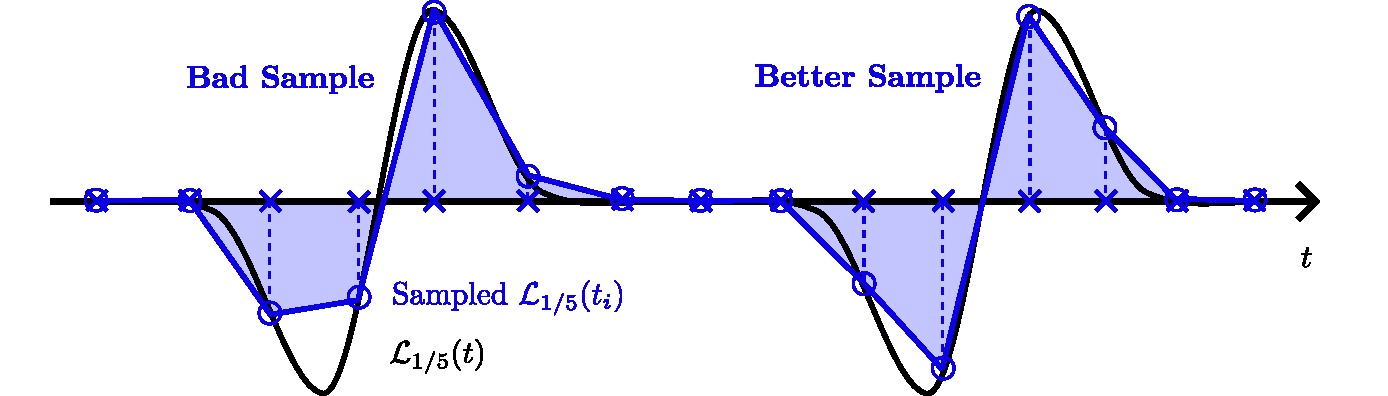
\includegraphics[scale=0.65]{assets/imgs/wave-sampling-comparison.pdf}
\caption{How ADCBCs might sample two Gaussian-shaped acoustic waves.}
\label{fig:wave-sampling}
\end{figure}

\fig{fig:wave-sampling} shows a representative analytic field $\cl{L}_{1, \rm{IN}}(t, y)$ for two acoustic bumps (which is roughly the derivative of a Gaussian). Despite a similar linear interpolation and sample period being used, the sampled $\overline{\cl{L}}_{1, s}$ values on the left are much worse than those on the right. The same could be true for any number of samples at a given interpolation order and sample period, where the change in phase and variability of the sampling will always cause some inaccuracy in the resulting integrated acoustic field upon reentry of these $\overline{\cl{L}}_{1, s}$ values. This inaccuracy results in a change to the shape of the disturbance which entered, e.g. a skew to one side, dissipation of acoustic energy or a drift in pressure and velocity behind the bump. These effects feed back into this issue at future bounces such that the waves eventually fully break down. Hence, small inaccuracies in integrated acoustic fields at reentry at the beginning of a simulation can result in large inaccuracies after more bounces. Note that the use of an acoustically conservative method for the ADCBCs would solve the issue of acoustic dissipation and pressure drift, but the destruction of the wave shape would not be. But, if the bump remains the same size and the tube is made longer, proportionally less bounces happen and the sampling error grows slower. Mathematically, if we begin with an error $\rm{err}_0$ which is amplified by $(1 + a)$ each bounce for some $a > 0$, then after $n$ bounces we have:
\begin{equation}
\rm{err}_A(n) \equiv (1 + a)^{n} \rm{err}_0.
\end{equation}
Thus, if the tube lengthens by a factor $b \equiv l_B / l_A > 1$, we instead expect to get only $n_B \equiv \lfloor n_A / b \rfloor$ bounces. This longer tube amplifies the error in the same way each bounce, so $\rm{err}_B(n) \equiv \rm{err}_A(n)$. Hence, the same number of bounces are required to reach the same error, or a time $t_B \approx b t_A$ to reach the same error. Considering this longer tube, we should acknowledge the longer associated frequencies of acoustic mode will be sampled many more times, meaning each bounce amplifies error instead by a factor $(1 + a / b)$ instead. In this case:
\begin{equation}
\rm{err}_C(n) \equiv \left( 1 + \frac{a}{b} \right)^n \rm{err}_0
\end{equation}
so $\rm{err}_C(n_C) = \rm{err}_B(n_B)$ if and only if $n_C \log(1 + a / b) = n_B \log(1 + a)$, or equivalently:
\begin{equation}
\frac{n_C}{n_B} = \frac{\log\left(1 + a\right)}{\log(1 + \frac{a}{b})} \xrightarrow{a \to 0^+} b
\end{equation}
so $b$ times more bounces are required to reach the same error or a time $t_C \approx b t_B$ in the asymptotic regime $a \ll 1$. Combined, these two effects result in a scaling of $t_C \approx b^2 t_A$. This quadratic scaling means that which are well-resolved by the ADCBCs in a short domain are very likely to be accurate in a long domain. Verifying the former, i.e. the usefulness of ADCBCs in short domains, is the premise of the the first two test cases in the coming chapter.




\cleardoublepage

\chapter{Numerical Validation} \label{ch:results}
As a preface to the following numerical validation, it should be mentioned that each of the test cases consist of two-dimensional rectangular domains with no objects in these domains. To be blunt this is a worst case for LABFM, which is a meshless method designed for its effectiveness in `interesting' geometries.

\emph{And rectangles are not interesting.}

Having said that, although the computational time may be larger than if, say, a simple centred finite difference method had been used due to the much larger stencil sizes, the use of LABFM here still provides discretisations with the high accuracy we require for the validation of the ADCBCs discussed in the previous chapter. Beyond this, there is something to be said for applying these new boundary conditions under less well-trodden conditions: if it works under LABFM, one would expect it also to work under more traditional methods.





\section{Acoustic Bump}

\begin{figure}[t]
\centering
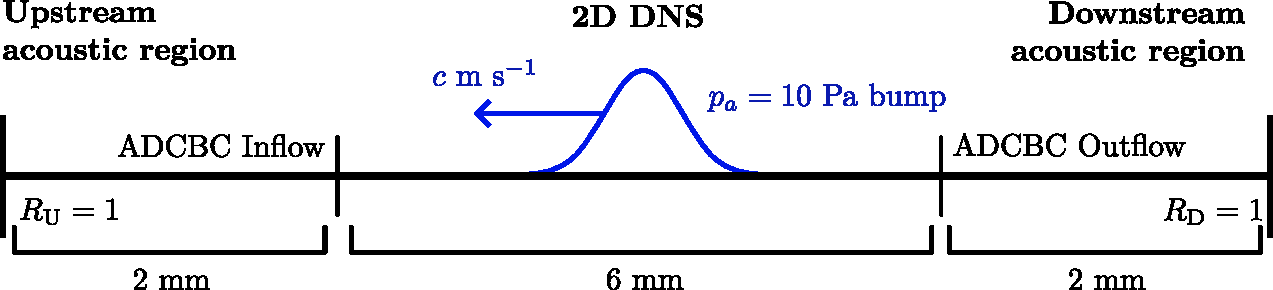
\includegraphics[scale=0.65]{assets/imgs/adcbc_bump_test.pdf}
\caption{The geometry and initialisation for the acoustic bump test case. Not drawn to scale.}
\label{fig:ac-bump-test}
\end{figure}

As our first test case, we model a Gaussian acoustic bump in a two-dimensional tube with two closed ends. The test case is initialised as a small bump in $J_1 \approx p' - ρ c u'$ (where the approximation comes from acoustic linearisation):
\begin{equation}
p_a(t = 0, x) = A \exp\left( - x^2 / d^2 \right)
\quad \text{and} \quad
u_a(t = 0, x) = p_a(t = 0, x) / ρ c
\end{equation}
such that the maximum pressure disturbance is $A = 10$ Pa and diameter $d = 2$ mm. This simple linear approximation also results in a small $J_5$ bump which we ignore. Alternate methods approximating this initial disturbance could also be used, although the provide little relevant improvement. Fluid properties are $u_{\rm{IN}} = 0.2$ m s$^{-1}$, $T_{\rm{IN}} = 298$ K and $p_{\rm{IN}} = 0.1$ MPa comprised of a single species with properties $W = 28$ kg kmol$^{-1}$, $Pr = 0.7$ and $c_p = 1100$ J kg$^{-1}$ K$^{-1}$. The resulting sound speed is $c \approx 348$ m s$^{-1}$. A 6 mm long central DNS region is used as well as up- and downstream acoustic regions modelled using ADCBCs on the inflow and outflow respectively, each modelling 2 mm of truncated tube. These essentially model two one-dimensional acoustic regions to the left and right of the flame. A diagram for this test case is shown in \fig{fig:ac-bump-test}. A sample rate of $δt_{\rm{sample}} \approx 0.25$ {\textmu}s is used for both ADCBCs and we use \nth{0} order interpolation (constant sample values) at the moment, for reasons discussed later. The horizontal top and bottom boundaries used in the DNS region are symmetric mirror boundaries, 1 mm apart. In total, there are 1224 collocation points in this domain processed by a single processor and 11 boundary nodes per boundary. With the linear acoustics equations in the acoustic regions being non-dispersive, we expect the Gaussian to retain its shape after each up- and downstream bounce. The full reacting Navier-Stokes equations are solved in the DNS region as a precursor to the a flame being present in the DNS region. Only in the DNS region should viscous effects alter the wave packet's shape and even in this case, only slightly after many bounces back and forth the 1 cm long domain. The ADCBCs work almost identically when the viscous inert, isothermal equations, which are also implemented into the SUNSET code, are solved. Note that the response to transverse effects are not being tested here because the acoustic is entirely one-dimensional. As mentioned above, we should in fact be modelling the convected wave equation, not the wave equation for quiescent fluids. But, since our Mach number, $\Ma < 10^{-3}$ is so low in this case the convective effects are deemed to be asymptotically unimportant. For thin regions like these, the boundary averaging procedure makes some physical sense as transverse behaviour at the boundaries of longer computational domains would be negligible, as it is here under our artificial test case. As the DNS domain widens, however, it seems reasonable that this averaging would result in more and more inaccuracy and potential instability. Hence, the queues are used for each boundary node should instead be used in this case to model many separate one-dimensional acoustic domains for each node. For all the cases in this report, the boundary averaging procedure is used and we find reassuring results regardless.

\begin{figure}[t]
\centering
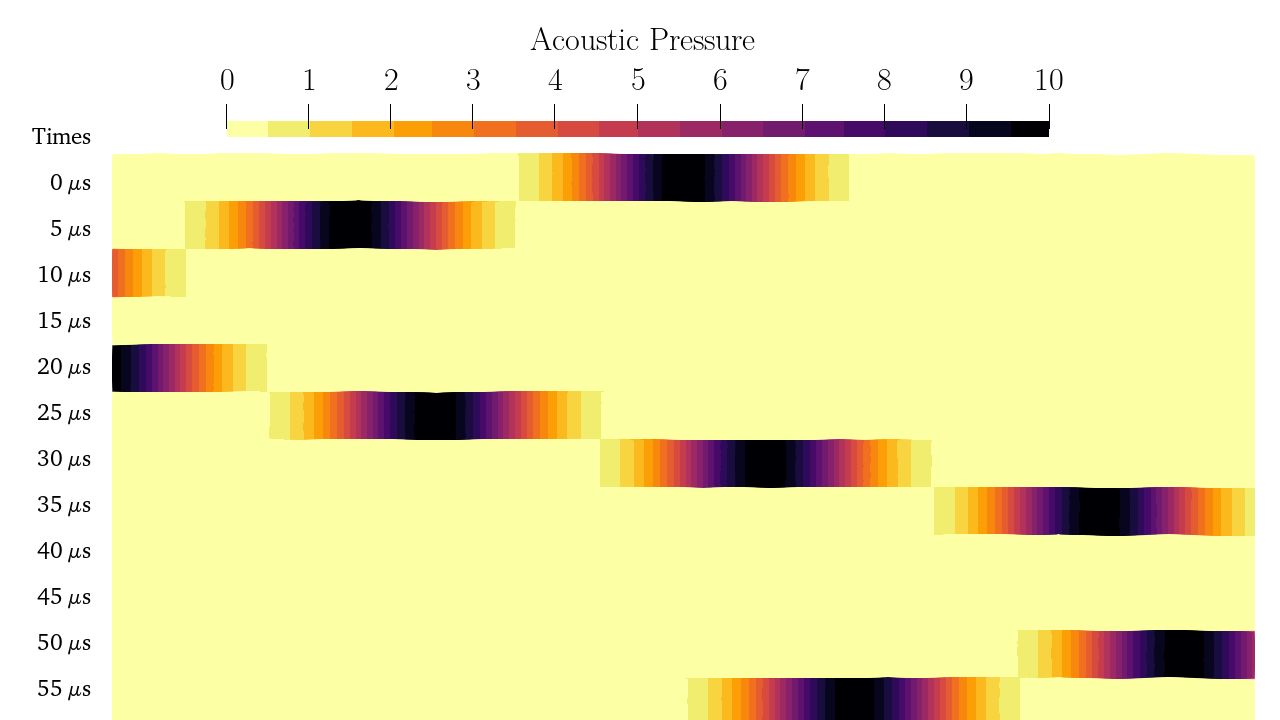
\includegraphics[scale=0.36]{assets/graphs/AC_BUMP_first_bounces_comp.png}
\caption{Acoustic pressure fields in the first 55 {\textmu}s in the DNS region in Pa. Only the top half of each DNS region is shown for comparison.}
\label{fig:ac-bump-dns}
\end{figure}

\begin{figure}[t]
\centering
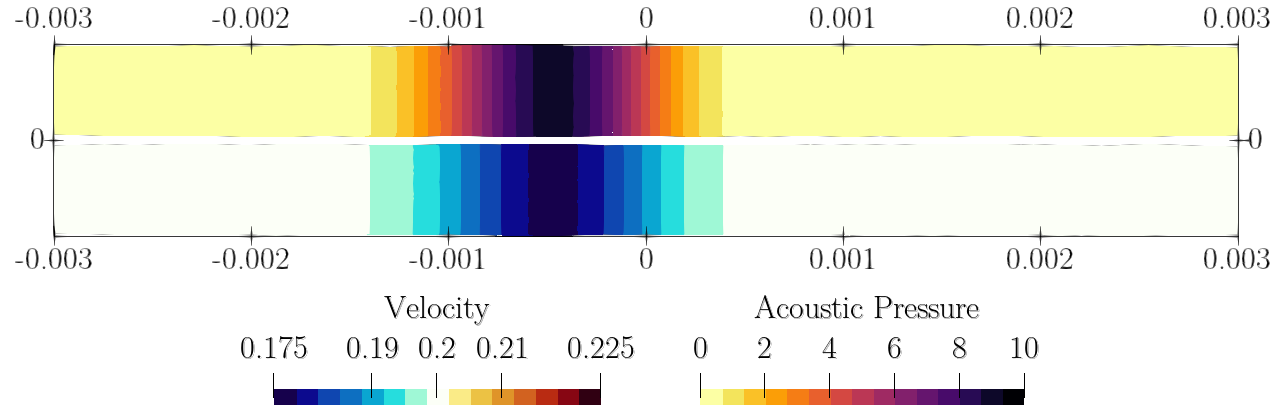
\includegraphics[scale=0.36]{assets/graphs/AC_BUMP_ndt=150e-4_comp.png}
\caption{$p_a$ and $u$ fields after 750 {\textmu}s in Pa and m s$^{-1}$. Here $u_a < 0$ so the acoustic is travelling left.}
\label{fig:ac-bump-dns-late}
\end{figure}

Pressure fields for the first bounces off the up- and downstream acoustic boundary are shown in \fig{fig:ac-bump-dns}. It seems after a single bounce off each end that the ADCBCs are adequately sampling and reintroducing the acoustic bump with negligible changes to its shape. The sample rate means that roughly $(d / c) / δt_{\rm{sample}} \approx 23$ samples are used to sample the first standard deviation of width of the Gaussian. This reconstruction of acoustic shape is impressive given the lack of interpolation (\nth{0} order interpolation means using constant sample values) used. After 750 {\textmu}s, the acoustic should have been sampled by the ADCBCs and reentered the DNS domain 13 times through each boundary. Note that up to this point in the simulation, the boundary conditions have taken up less than one percent of the overall simulation runtime. This is unsurprising given how few boundary nodes there are and since the bulk of the simulation time is spent calculating gradients at the other $\sim$1000 discretisation points. The pressure and velocity fields are shown in the DNS region at this time in \fig{fig:ac-bump-dns-late}. We can see that the size of highest acoustic pressure region has shrunk somewhat so some acoustic losses have been encountered. We note here that a better test of the ADCBCs would be to compare these results against a fully simulated 1 cm long tube with hard inflows and outflows given by specifying $u=0.2$ m s$^{-1}$ at these boundaries to model the closed boundaries. This analysis is not performed in this report. Regardless, it seems as though changes to the acoustic's shape are minimal despite the short acoustic length scale. Thus, from the previous chapter we know that this error should be minimised even farther when a longer tube is simulated. For example, if a 1 m long tube is simulated instead, we expect the same error to occur at roughly $t_C = (1~\text{m} / 1~\text{cm})^2 \cross 750~\text{{\textmu}m} = 7.5$ s in the longer simulation. This should be ample time to simulate a thermoacoustically unstable flame.

\begin{figure}[t]
\centering
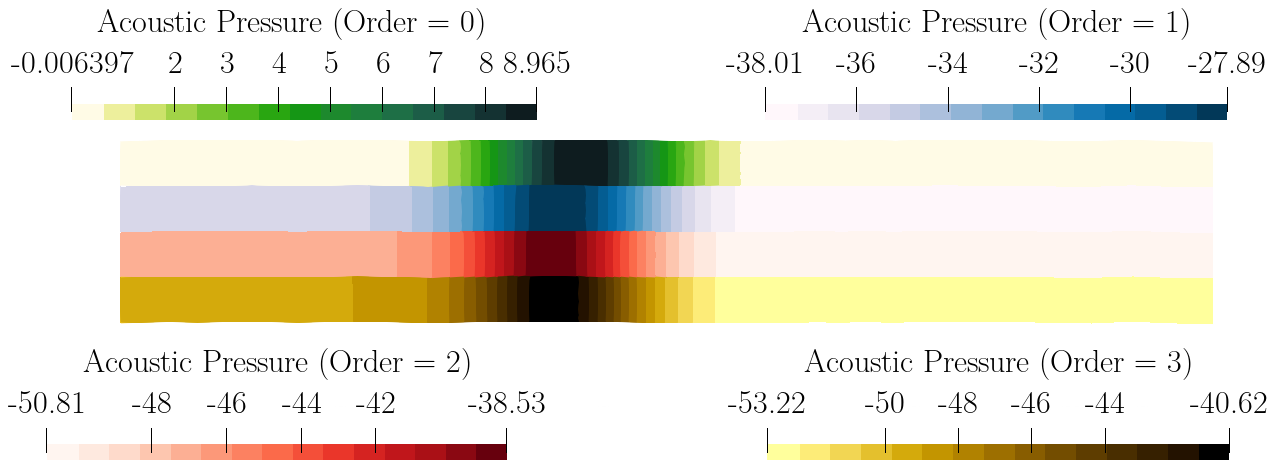
\includegraphics[scale=0.36]{assets/graphs/AC_BUMP_orders.png}
\caption{Acoustic pressures of the acoustic disturbance after 750 {\textmu}s for zero to third order interpolation (top to bottom) in Pa. Only the top half of each DNS region is shown for comparison.}
\label{fig:ac-bump-dns-orders}
\end{figure}

The above results are found provided constant interpolation is used to evaluate $\overline{\cl{L}}(t - τ)$ values. Results of the same Gaussian acoustic bump after 750 {\textmu}s for orders zero to three are shown in \fig{fig:ac-bump-dns-orders}. Bizarrely, when higher orders of interpolation are used the results massively deteriorate and large amounts of error are introduced each every bounce. After the thirteen bounces, we are left with an acoustic bump of roughly the same size $\max(p_a) - \min(p_a) \approx 10$ Pa, but with a drift in pressure much larger than this. Clearly this pressure drift is the result of the pressure difference between the front and back of the bump adding up after repeated bounces, which is most likely caused by the sampling error introduced in the previous chapter since the boundary averaging procedure should be having little to no effect in this quasi-one-dimensional test case. Although, it is unclear why this happens only when non-constant interpolation is used. Assuming it isn't the result of a mistake in the ADCBCs implementation into the SUNSET code, there is potentially some term in the error of the reintegrated acoustic upon reentry which is cancelled out when constant sample values are used, but not for interpolated values. Either way, this needs to be investigated further.

\begin{figure}[t]
\centering
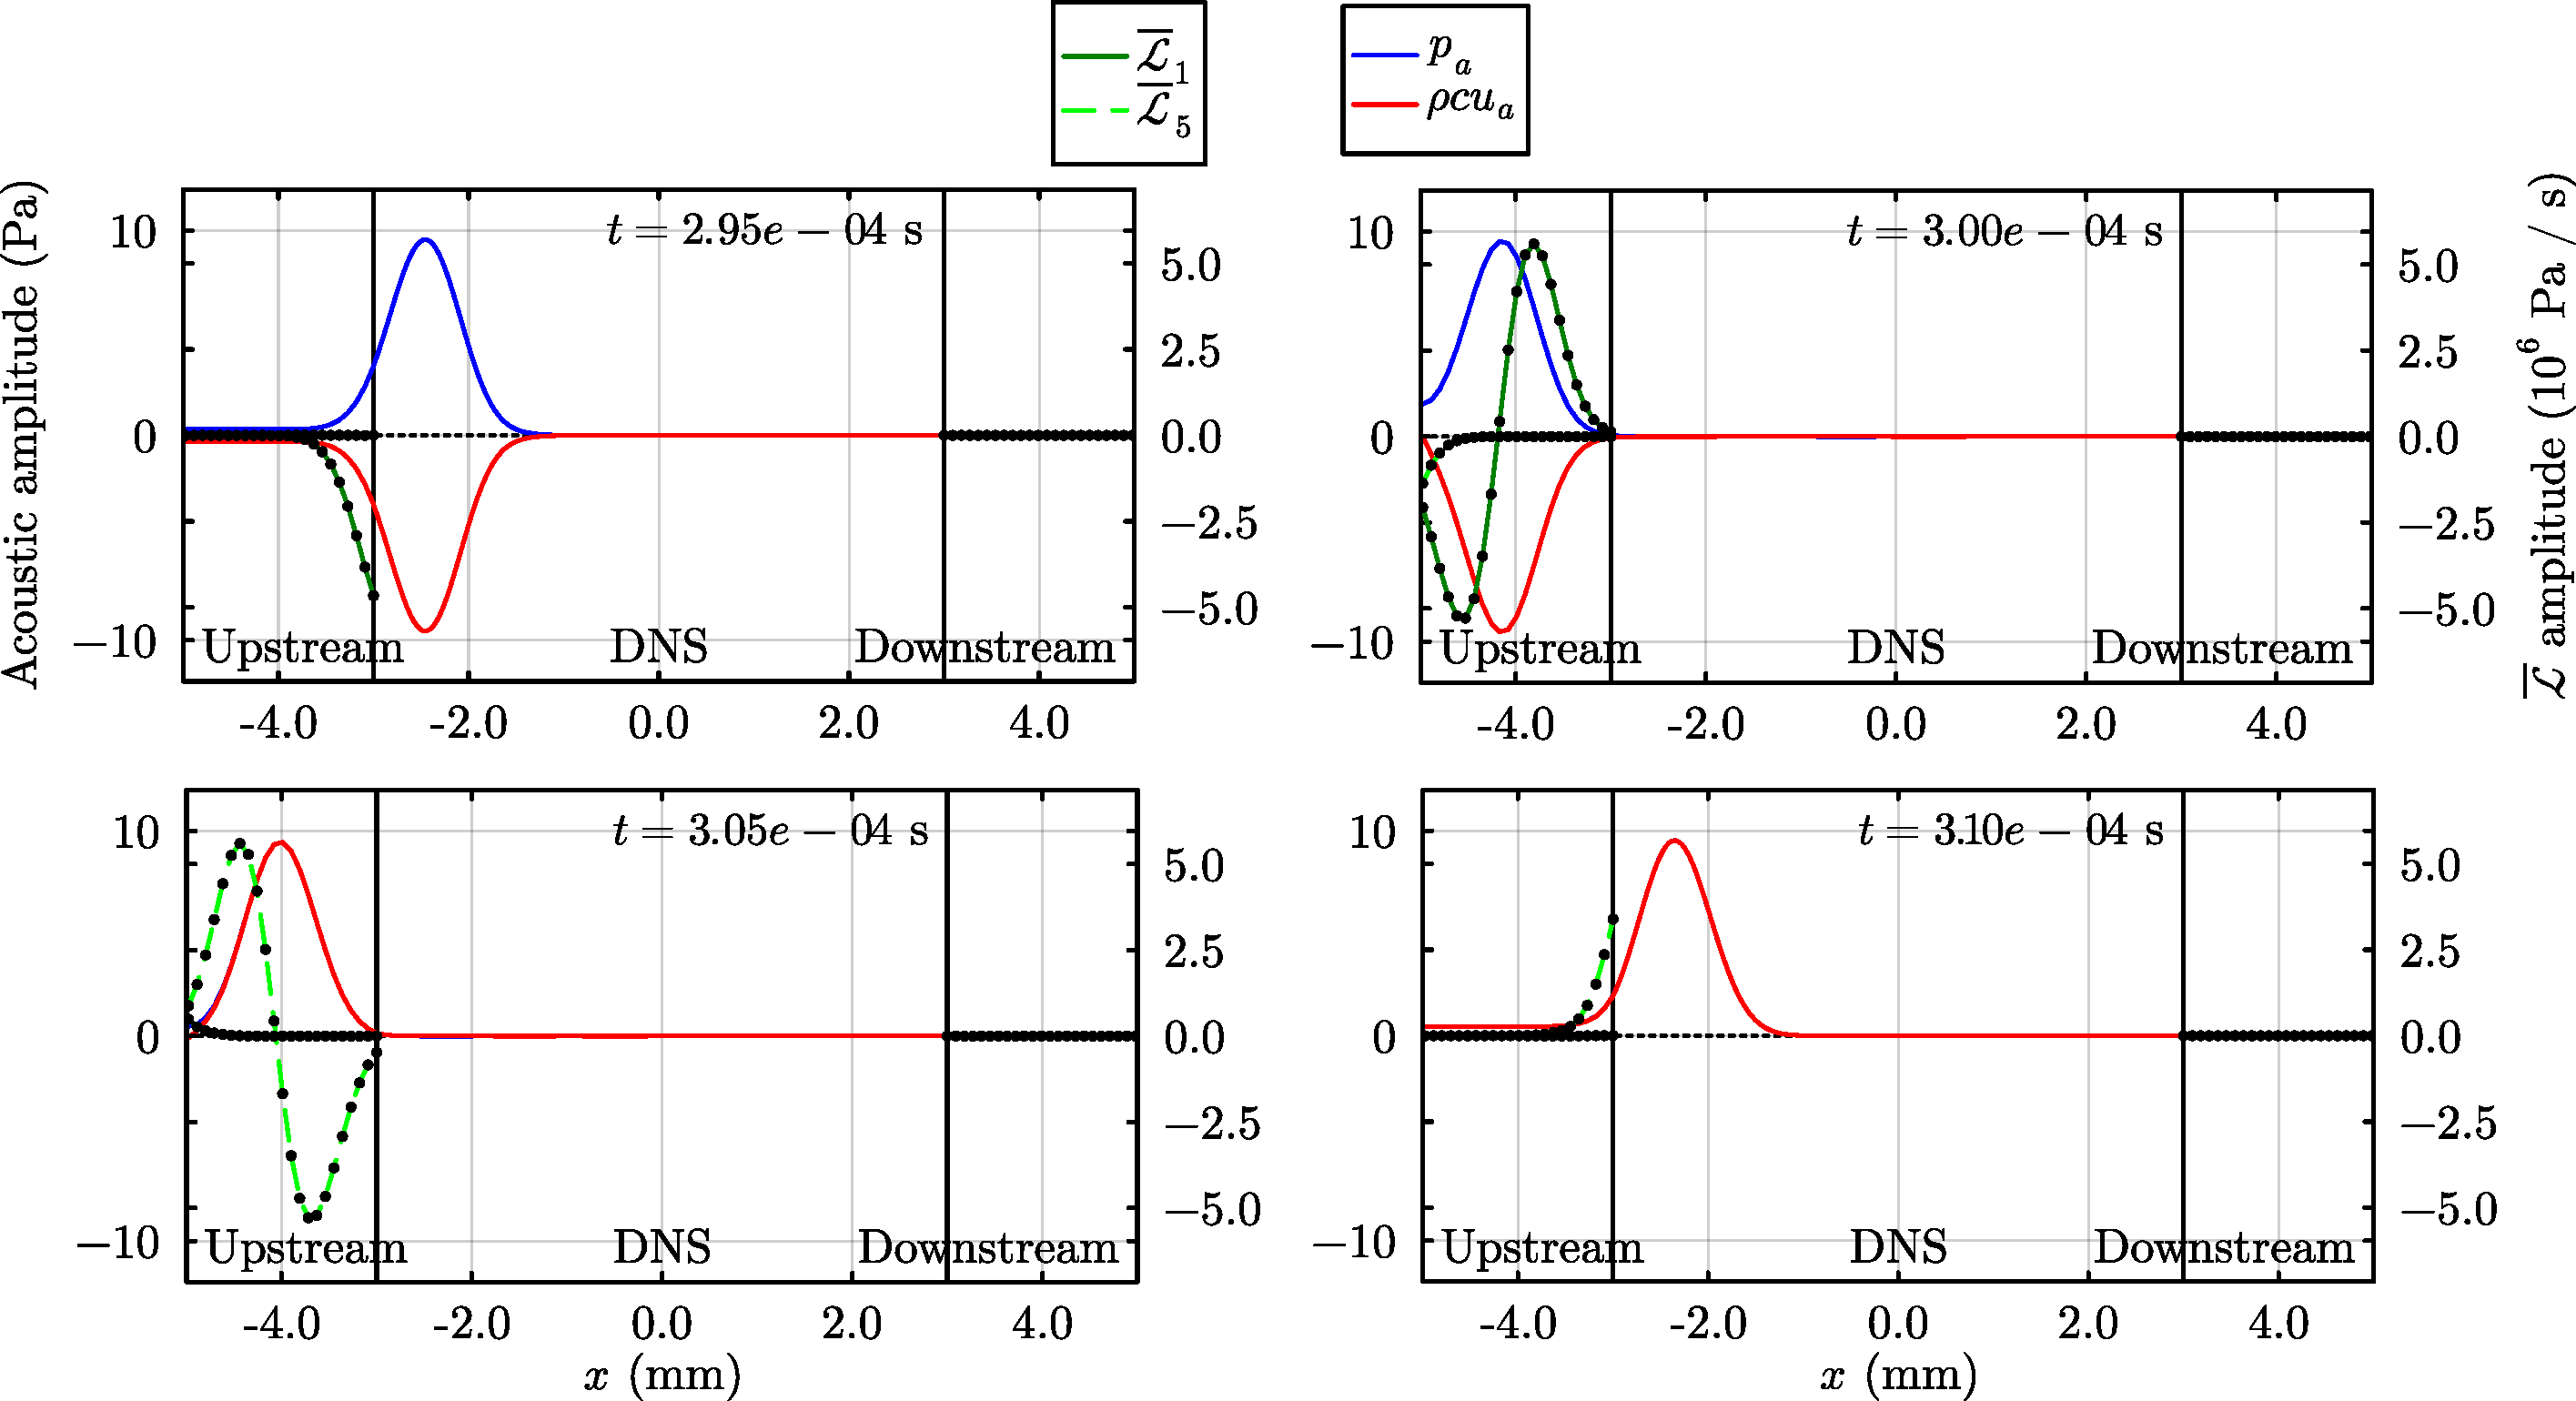
\includegraphics[scale=0.35]{assets/graphs/ac_frames_order=0.pdf}
\caption{Reconstruction of the acoustic fields in the acoustic and DNS regions for the simulation using zeroth order interpolated samples.}
\label{fig:ac-reconstruct_order0}
\end{figure}

\begin{figure}[t]
\centering
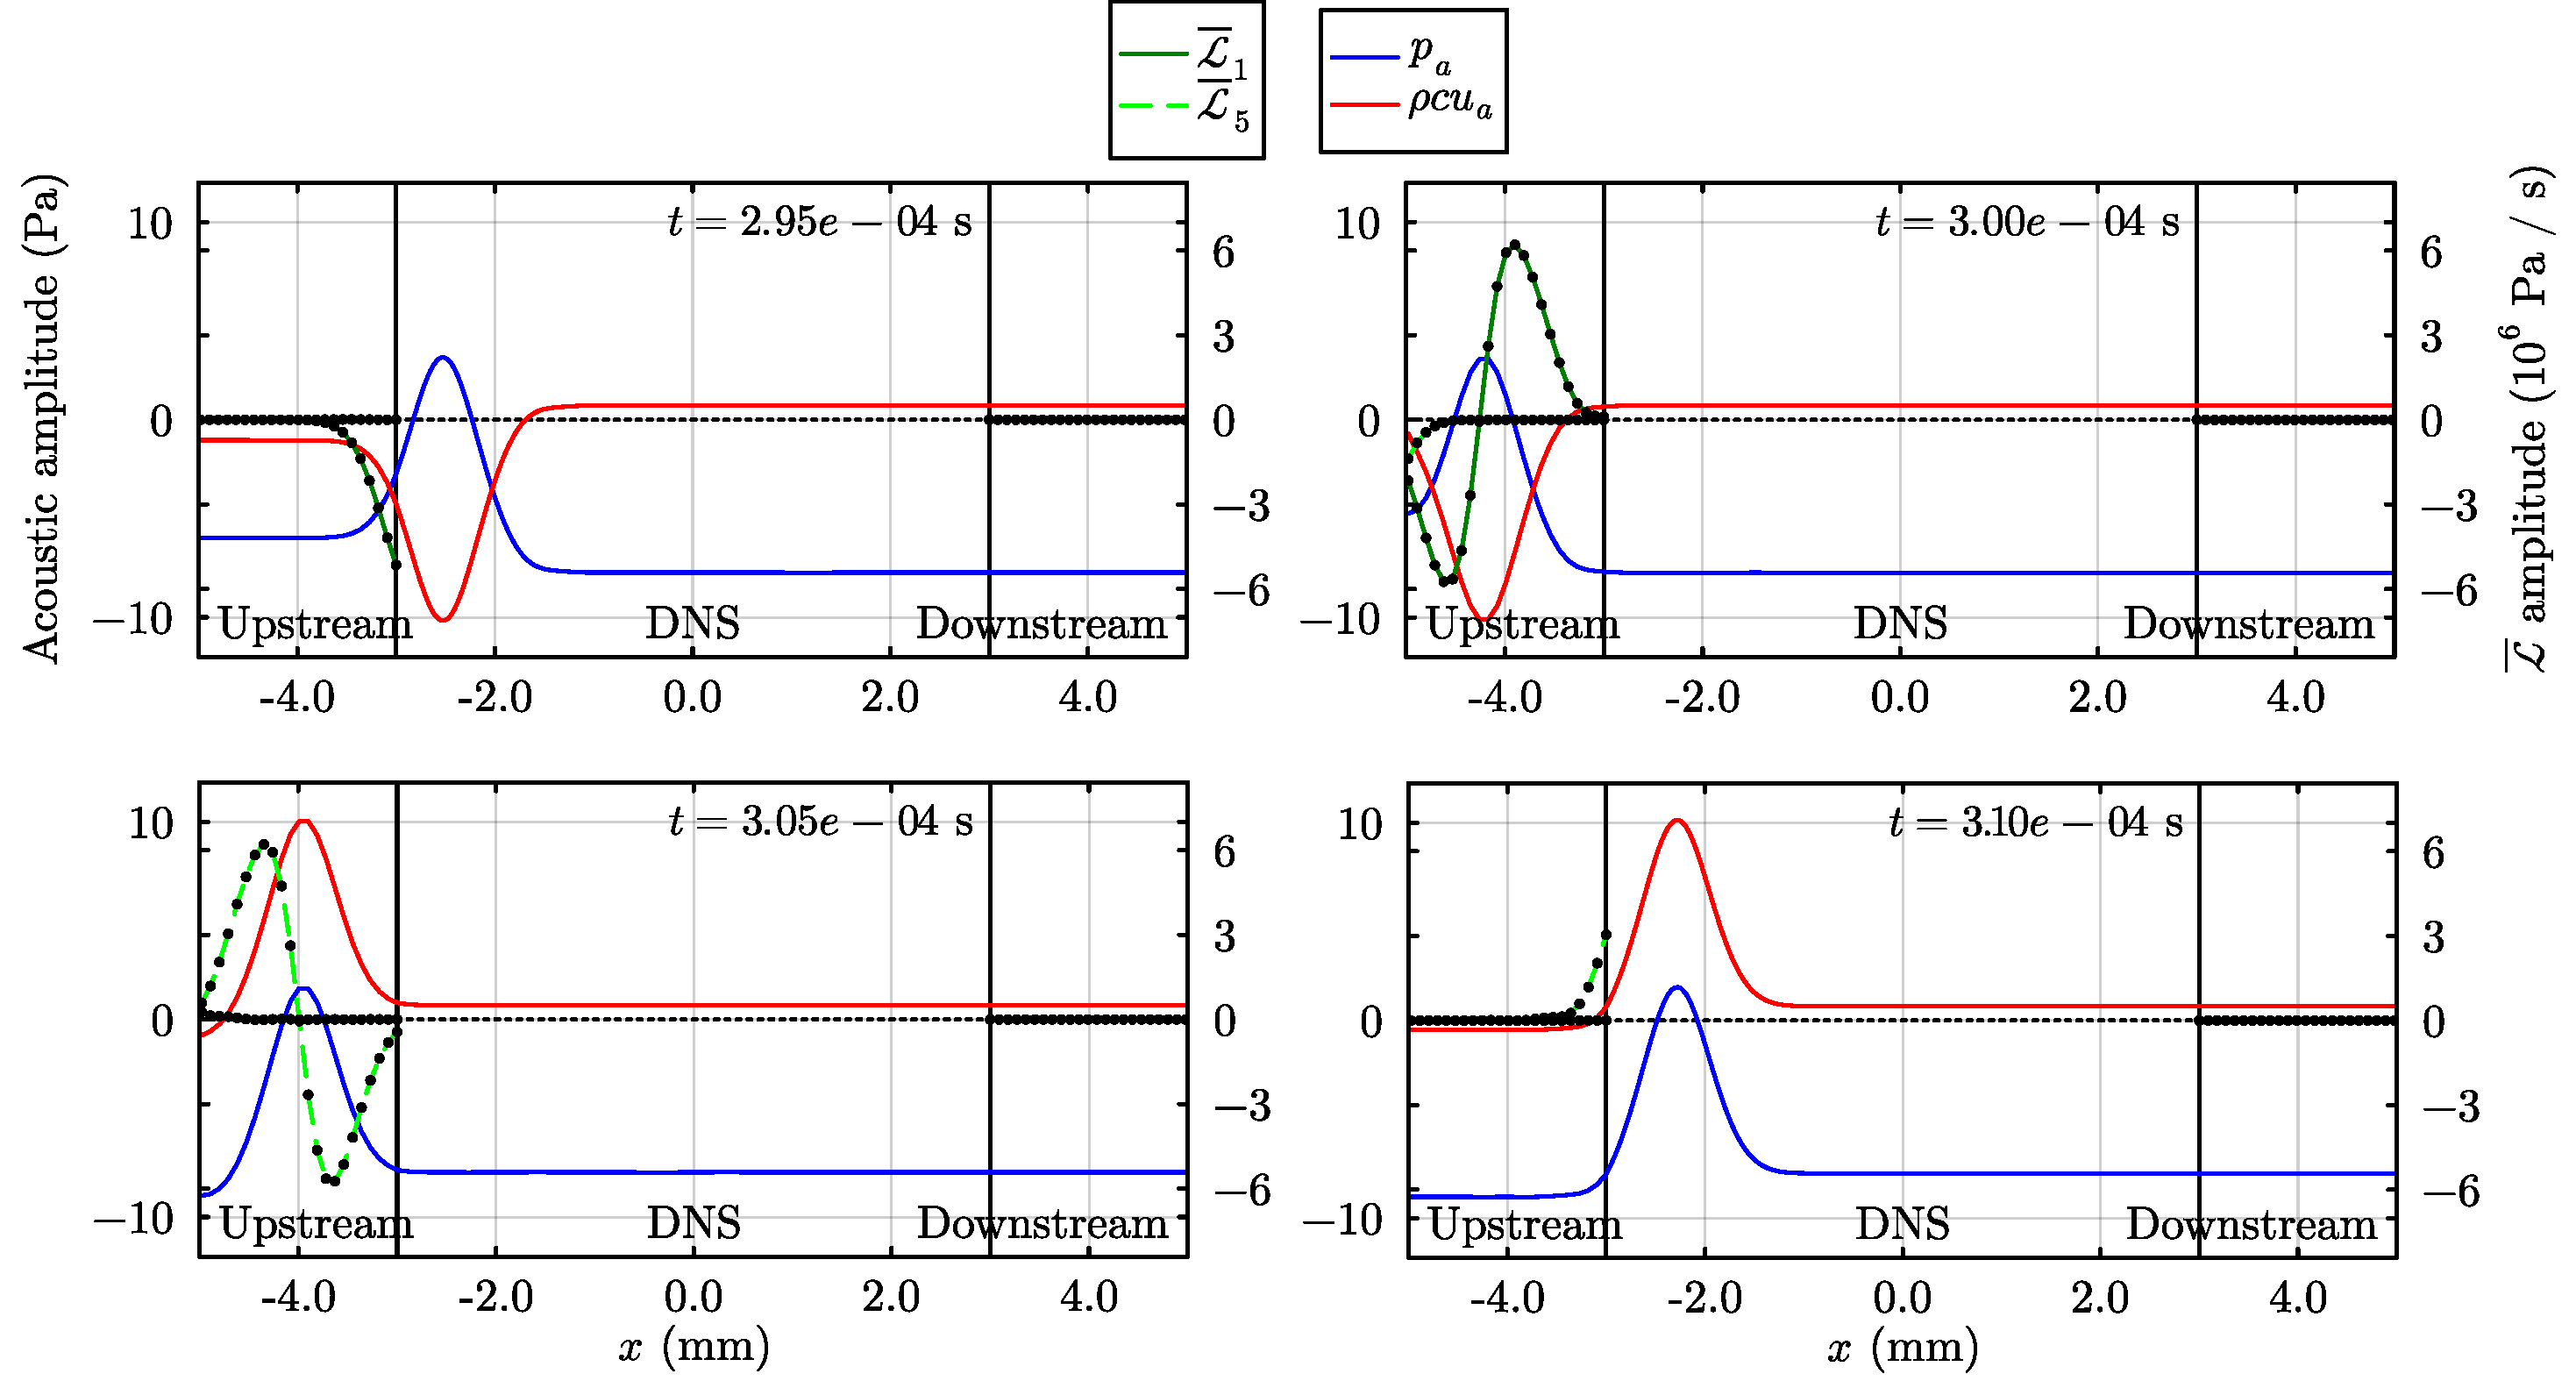
\includegraphics[scale=0.35]{assets/graphs/ac_frames.pdf}
\caption{Reconstruction of the acoustic fields in the acoustic and DNS regions for the simulation using third order interpolated samples.}
\label{fig:ac-reconstruct_order3}
\end{figure}

We can now use the discretised acoustic region field reconstruction from the previous chapter to observe the acoustics in the fictitious region in a way which is not immediately available to us from the interior DNS data. In \fig{fig:ac-reconstruct_order0} are the results for the constant interpolation, where we see although the acoustic field has dissipated by $\sim$1 Pa, the symmetric Gaussian structure is maintained. Instead, in \fig{fig:ac-reconstruct_order3} an asymmetric structure resulting in the pressure drift mentioned above. The values of $\cl{L}$ in both figures showcase these values moving with $p_a$ and $u_a$ in the upstream acoustic domain, which is roughly $\propto ζ \exp(-ζ^2)$ for some variable $ζ(t, x)$. Notice that because $R_{\rm{U}} = 1$ in both cases we get that $\cl{L}_{5, \rm{U}}(t, x_{\rm{IN}} - l_{\rm{U}}) = \cl{L}_{1, \rm{U}}(t, x_{\rm{IN}} - l_{\rm{U}})$. This should always result in the Dirichlet condition $u_a(t, x_{\rm{IN}} - l_{\rm{U}}) = 0$ and Von Neumann condition $\partial p_a / \partial x(t, x_{\rm{IN}} - l_{\rm{U}}) = 0$, althoug we notice that this is not true for the third order simulation. In the case where an open acoustic boundary $R_{\rm{U}} = -1$ is used instead, we have $\cl{L}_{5, \rm{U}}(t, x_{\rm{IN}} - l_{\rm{U}}) = -\cl{L}_{1, \rm{U}}(t, x_{\rm{IN}} - l_{\rm{U}})$ so the boundary conditions on $p_a$ and $u_a$ swap. Both these cases match the desired acoustic properties for open and closed tubes under typical acoustic modelling.




\section{Acoustic Standing Wave}

\begin{figure}[t]
\centering
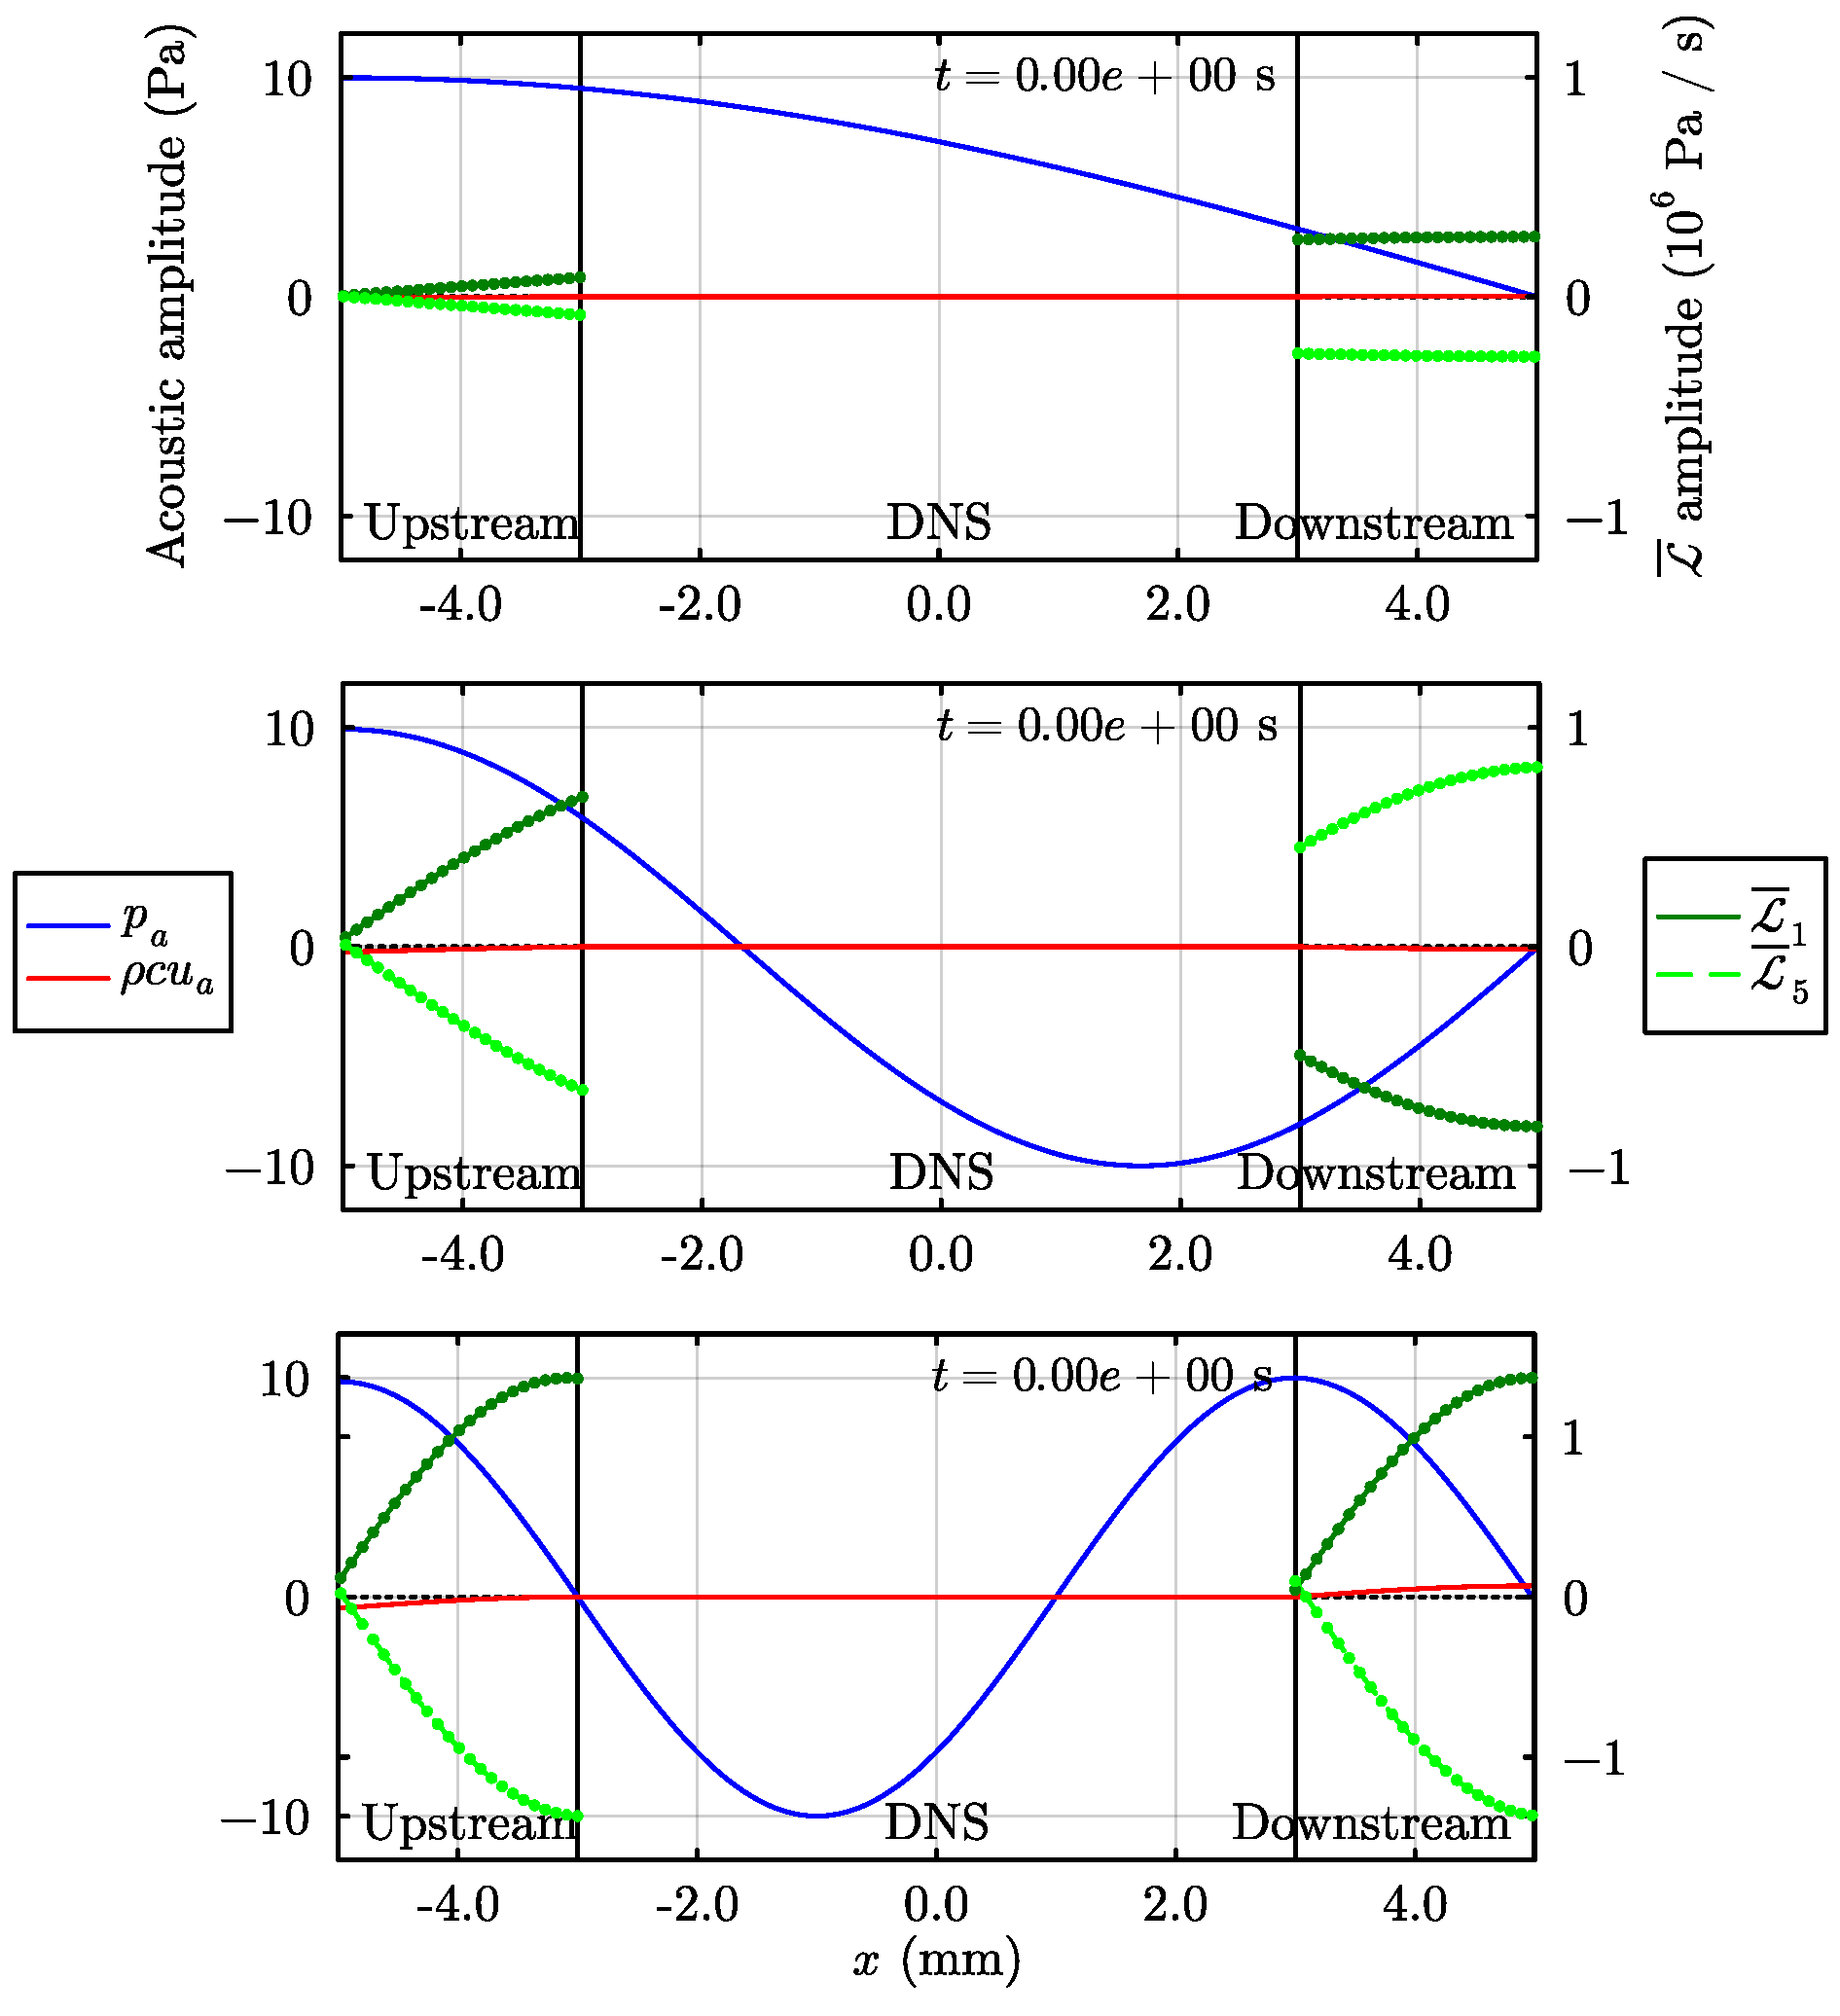
\includegraphics[scale=0.35]{assets/graphs/ac-plot-wave-modes.pdf}
\caption{Reconstruction of the initial acoustic fields for $N_κ = 1, 2, 3$.}
\label{fig:ac-wave-modes}
\end{figure}

\begin{figure}[t]
\centering
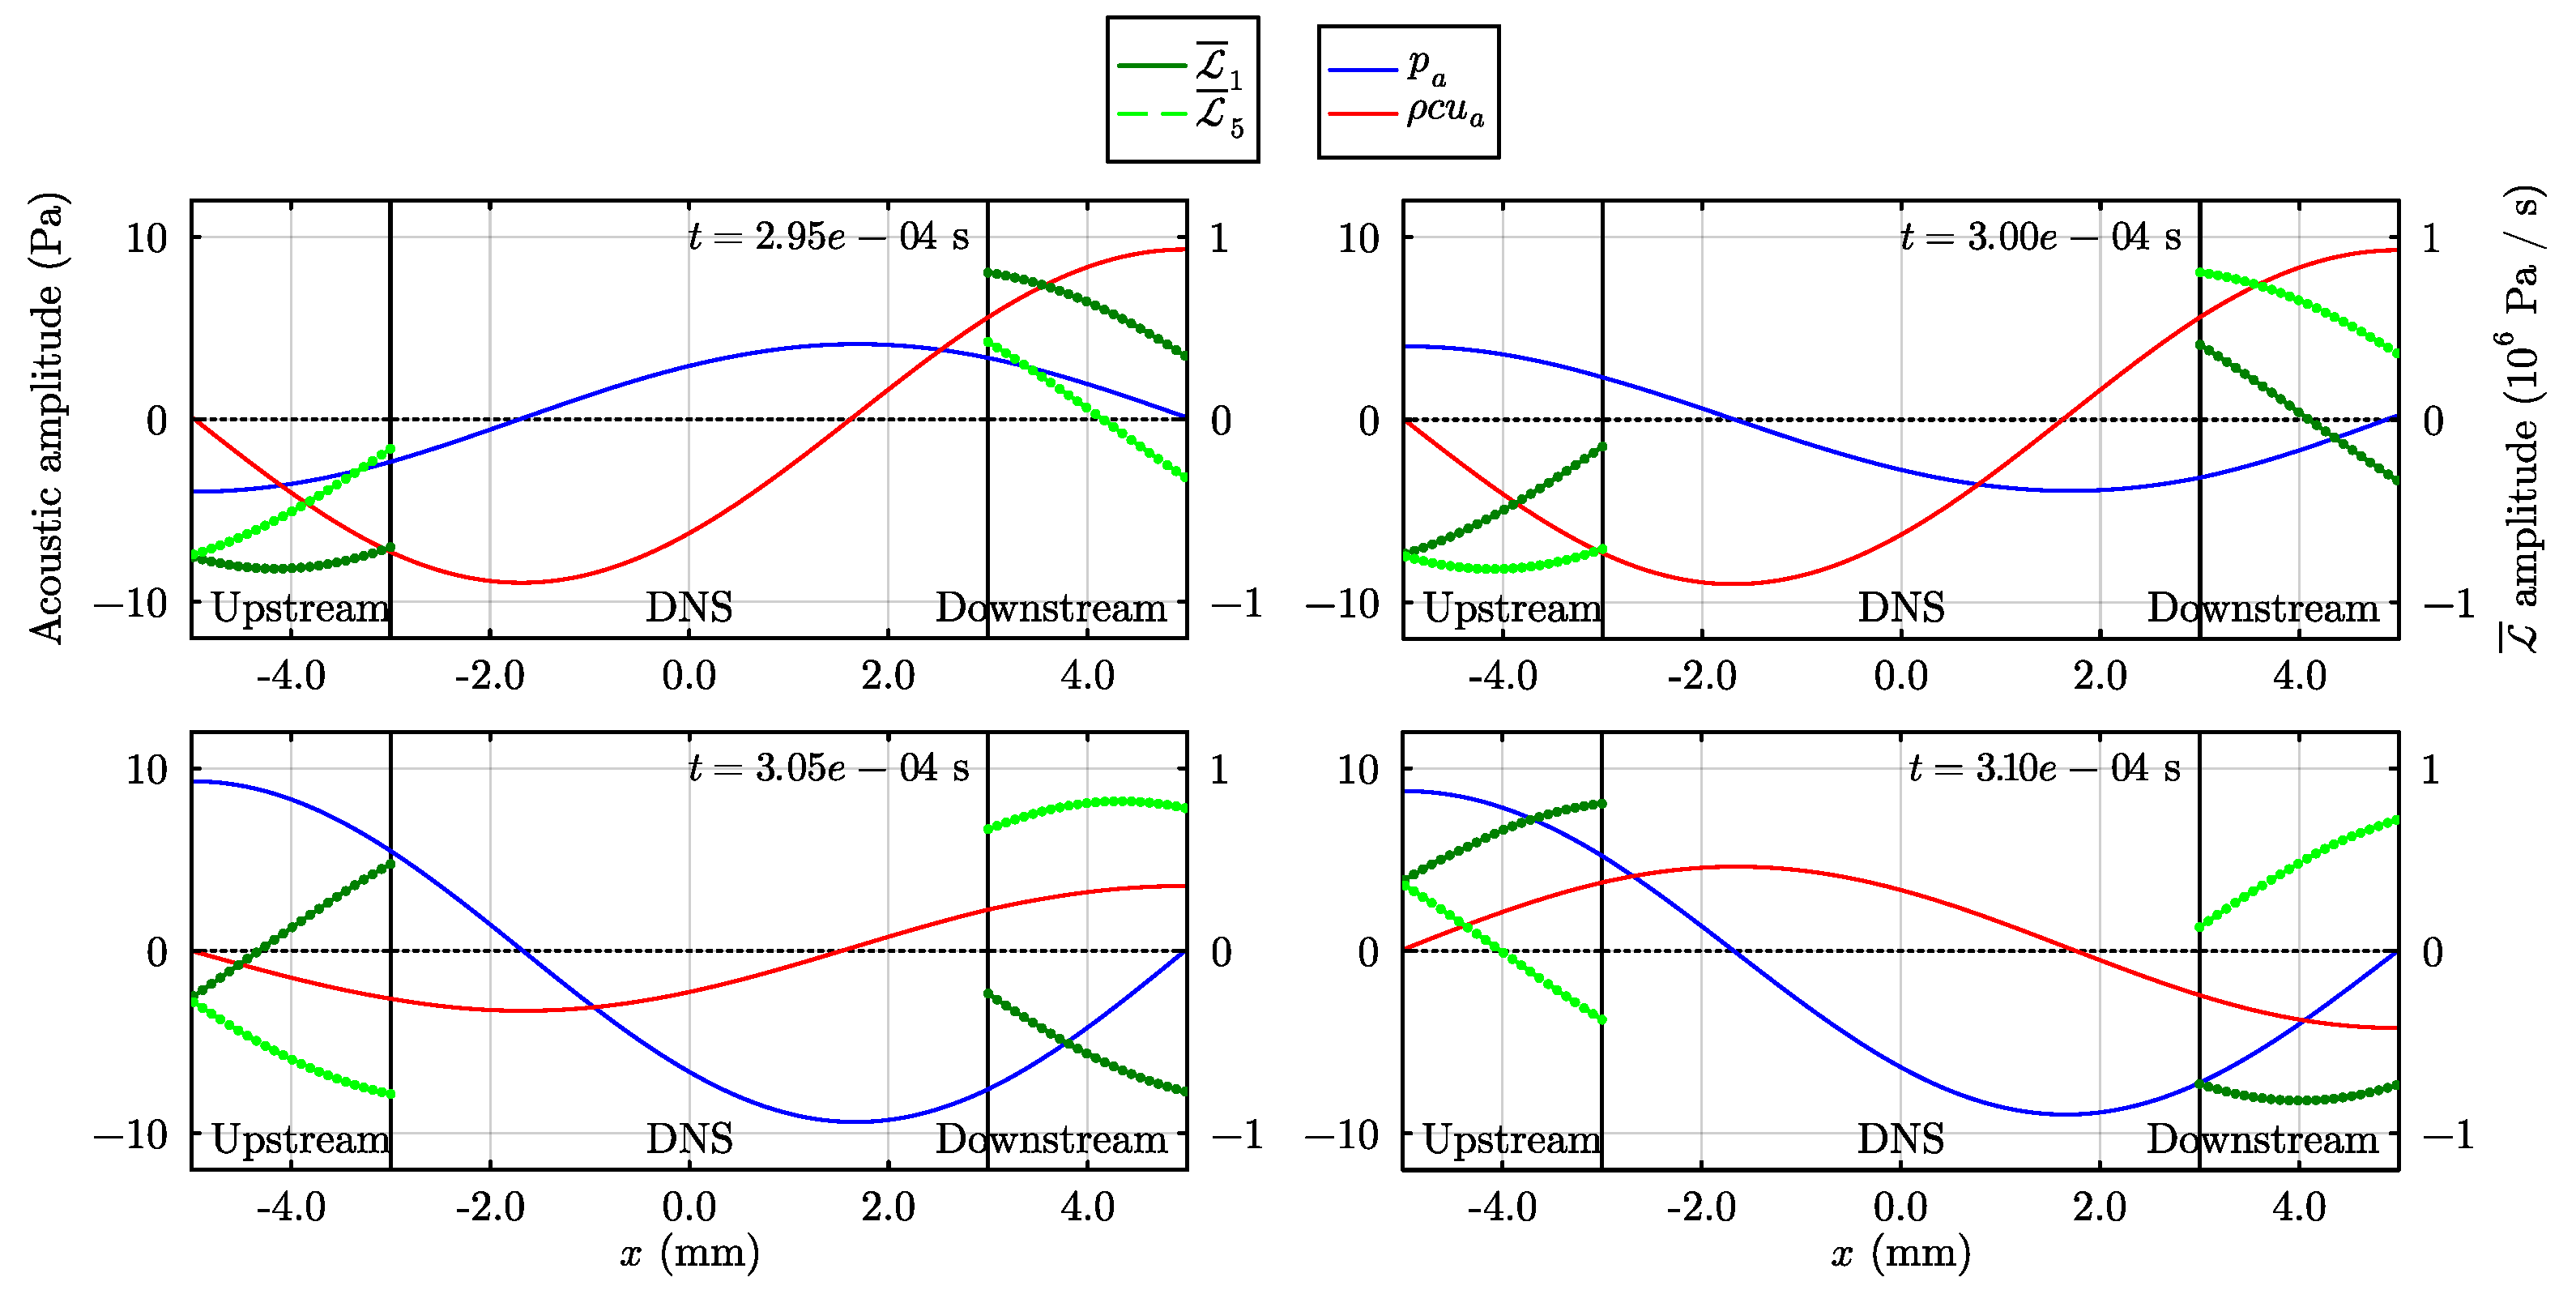
\includegraphics[scale=0.33]{assets/graphs/ac-plot-3-4_long.pdf}
\caption{Reconstruction of acoustic fields for $N_κ = 2$.}
\label{fig:ac-wave-later}
\end{figure}

We now initialise an acoustic standing wave in the same computational domain as the previous test case, using the same fluid properties and ADCBC parameters, except for the change that we instead model an open upstream acoustic boundary, so $R_{\rm{D}} = -1$ instead and we use constant interpolation. The desired initial acoustic pressure is:
\begin{equation}
p_A(t = 0, x) = A \cos\left( 2 π \, \frac{x - x_{\rm{IN}} - l_{\rm{U}}}{l_{\rm{tube}}}  \, \frac{2N_κ - 1}{4}\right),
\end{equation}
where $A = 10$ Pa is the acoustic amplitude as before and $l_{\rm{tube}} \equiv l_{\rm{U}} + (x_{\rm{OUT}} - x_{\rm{IN}}) + l_{\rm{D}}$ is the full tube length with $l_{\rm{U}} = l_{\rm{D}} = 2$ mm and $(x_{\rm{OUT}} - x_{\rm{IN}}) = 6$ mm. $N_k$ determines the wavenumber of the standing wave: if $N_κ = 1$ we have the $1 / 4$ mode, if $N_κ = 2$ we have the $3 / 4$ mode etc.. The corresponding wavenumber is:
\begin{equation}
κ = \frac{2N_κ - 1}{4 l_{\rm{tube}}}
\end{equation}
In the DNS region, the wave can be initialised by directly calculating $p_a(0, x)$ values. In the upstream and downstream region, however, we must instead calculate $\cl{L}_{1/5}(t = 0, x)$ using the formulae in \equ{eqn:λ_l_L}, discretise them and enter the resulting finite values into the initial queues $(\bb{T} \cross \bb{L})(t = 0)$ for the ADCBC inflow and outflow. \fig{fig:ac-wave-modes} shows the acoustic initial conditions in the full tube for the first three standing wave modes. In each of the three graphs, the wave continues smoothly into the acoustic domain owing the acoustic reconstruction introduced in the previous chapter. \fig{fig:ac-wave-later} shows the simulation after a few acoustic periods for the $N_κ = 2$ case. Clearly $u_a(t, x_{\rm{IN}} - l_{\rm{U}}) = 0$ and $p_a(t, x_{\rm{OUT}} + l_{\rm{D}}) = 0$ as desired. In this case you can see the reconstructed $\cl{L}_{1/5}$ fields travelling left and right respectively. Note that in the $N_κ = 2$ and 3 modes you can see a slight error with some $u_a(t = 0, x) \ne$ values in the up and downstream domain due to inaccuracies with the post-processing code.

\begin{figure}[t]
\centering
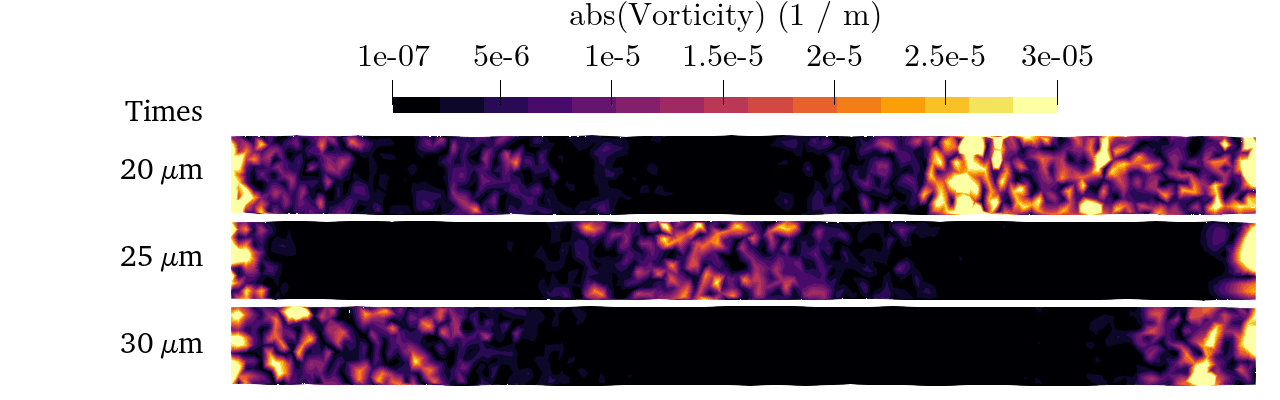
\includegraphics[scale=0.36]{assets/graphs/AC_WAVE_QWAVE.png}
\caption{Spurious vorticity wave travelling through the DNS domain at the acoustic speed for the $N_κ = 2$ wave.}
\label{fig:vort-wave}
\end{figure}

Focusing instead on the DNS region, looking only at vorticity disturbances -- given that the background vorticity should be $\vb{ω} \equiv \vb{\nabla}\cross\vb{u} \equiv 0$ for the one-dimensional flow -- we can see in \fig{fig:vort-wave} a vorticity perturbation travelling at the acoustic speed, right to left. This can also be seen in disturbances to $v$. Not depicted in the figure is this wave and another bouncing back and forth through the DNS domain, as if it is being transmitted through the full acoustic domain. This is likely the result of the $\cl{O}(h^k)$
The simplest explanation for this `error' wave is 
Note the larger values of $\abs{\vb{ω}}$ at the characteristic boundaries due to variations of $u$ and $\cl{L}_{1/5, \rm{nonreflect}}$ along the boundary.

% Sampling error
% - We can also see the sampling instability in the standing wave results as a q-wave \cite{poinsot2001TheoreticalNumericalCombustion} which is largest at maximum values of L???
% - Show image/s. Easiest to see when instability is not present
% - We can find similar results for standing waves as a bump in terms of interpolation order?
% - Once again, for tubes which are long enough this should not be a concern due to the quadratic growth of period with length. This is consistent with our results in the next section



% We use SI units (1 / m)
\begin{figure}[t]
\centering
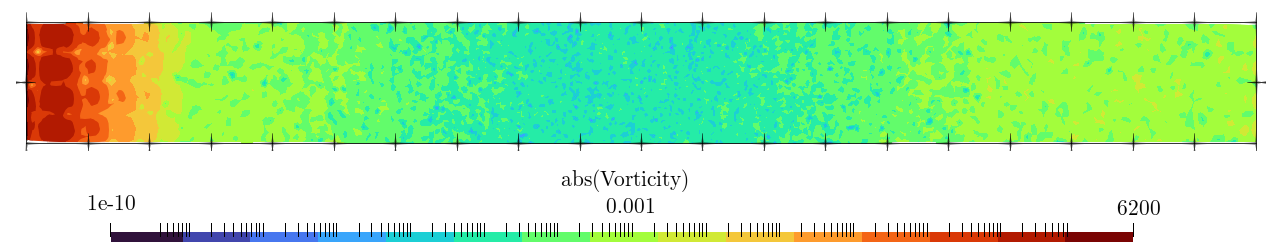
\includegraphics[scale=0.36]{assets/graphs/u-inflow-instab.png}
\caption{INFLOW INSTAB}
\label{fig:inflow-instab}
\end{figure}



% Instability issue!
% - We observed that under certain boundary discretisations, a wringing instability of u develops at the inflow after many acoustic periods. This grows exponentially, suggesting the instability behaves linearly, until the vorticity produced within the DNS region destroys the solution
% - Show image!!
% - This instability can be reduced by increasing the coefficient of the hyperviscosity filter at the inflow boundary nodes. Specifically, by increasing the hyperviscosity tangential to the inflow, the wringing mode is dampened to the point that it cannot grow
% - for us, we..
% - This instability may or may not show up when multiple queues are used for each inflow/outflow, so this needs to be investigated. It appears to be largely a result of the boundary averaging procedure.




% Moving domain results
% - shows validation that the delay time can indeed change
% - time scale for delay change is much longer due to the low Mach number
% - Show two images at separate times where the domain has moved but the acoustic remains well-resolved




\section{Thermoacoustically Unstable Flame}

\begin{figure}[t]
\centering
    \begin{subfigure}{0.99\textwidth}
    \centering
    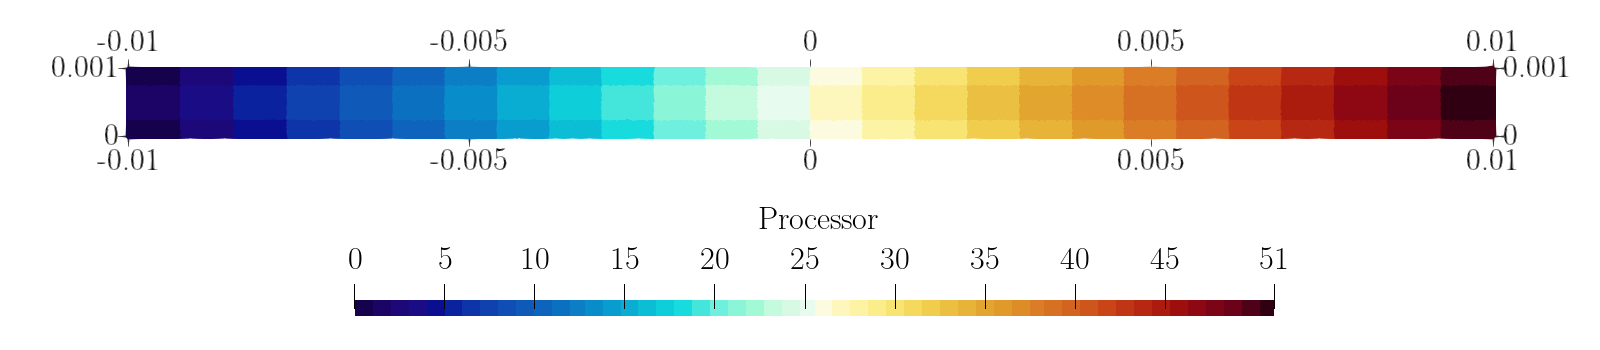
\includegraphics[scale=0.25]{assets/graphs/flame-sim-discretisation.png}
    \caption{}
    \label{fig:disc1}
    \end{subfigure}

\vspace*{0.5em}

    \begin{subfigure}{0.99\textwidth}
    \centering
    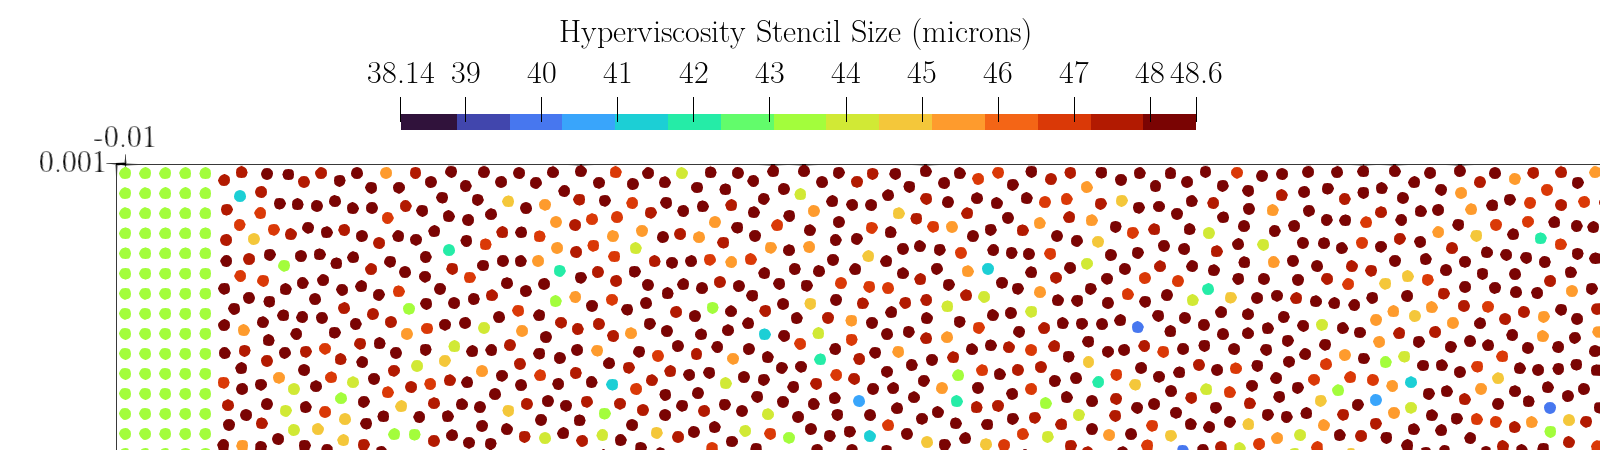
\includegraphics[scale=0.25]{assets/graphs/flame-sim-discretisation_zoom.png}
    \caption{}
    \label{fig:disc2}
    \end{subfigure}
\caption{DNS COMPUTATIONAL DOMAIN}
\label{fig:disc}
\end{figure}

% We now study a thermoacoustically unstable flame in a reflected DNS domain shown in fig ..
% Flame properties are: single step irreversible reaction with fluid properties constant in reactants and products, q = 6, Ze = 5, S_L = u_in = 0.2 m / s, Le = 1, with derived laminar flame thickness l_L = 0.216 mm
% Even though LABFM enables variable resolutions, we use constant discretisation length scale for these simulations as we don't know where the flame will end up a priori. A discretisation length scale of $s = 18$ μm is used and w = 2mm.
% Show the discretisation used zoomed in and out!
% It may seem like a large jump to go from inert, essentially isothermal acoustics to fully reacting flame-acoustic interactions, but the sunset code is designed with flame simulations in mind, so the simulations are 'easy' to perform having already implemented ADCBC.
% (Maybe there are better intermediate test cases? D-TDIBC don't seem to need them)



\subsection{Acoustic Eigenmodes}

% Prediction from Eigenmodes
% - First we predict what results we get in a one-dimensional closed-open tube of the same length under the linear acoustic approximation, modelling the flame as a discontinuity which does not interact with the acoustics.
% First take the non-dimensionalised equations for compressible, inviscid fully non-linear flow:
% ... (continue on with maths)

\begin{figure}[t]
\centering
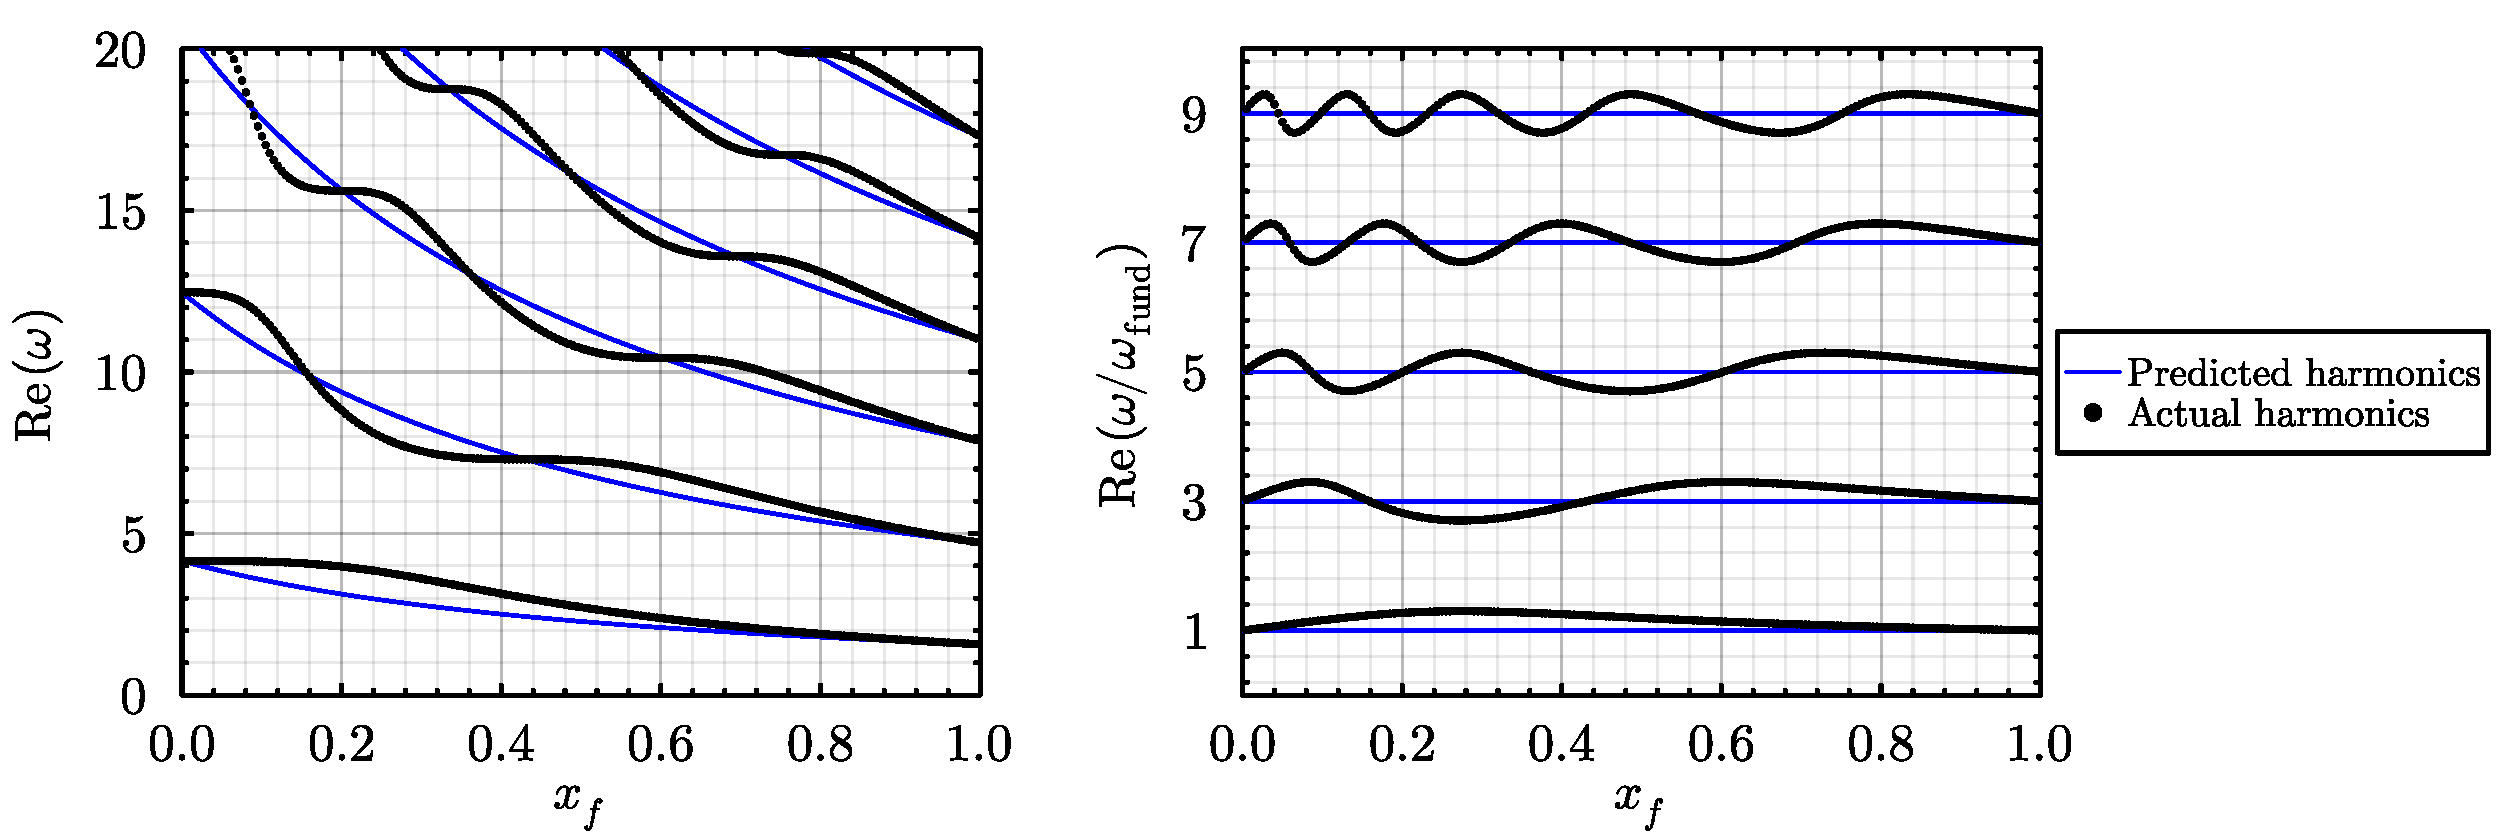
\includegraphics[scale=0.35]{assets/graphs/r=7_harmonics_both.pdf}
\caption{$r = 7$, LEFT: , RIGHT: divided by }
\label{fig:flame-harmonics}
\end{figure}

\begin{figure}[t]
\centering
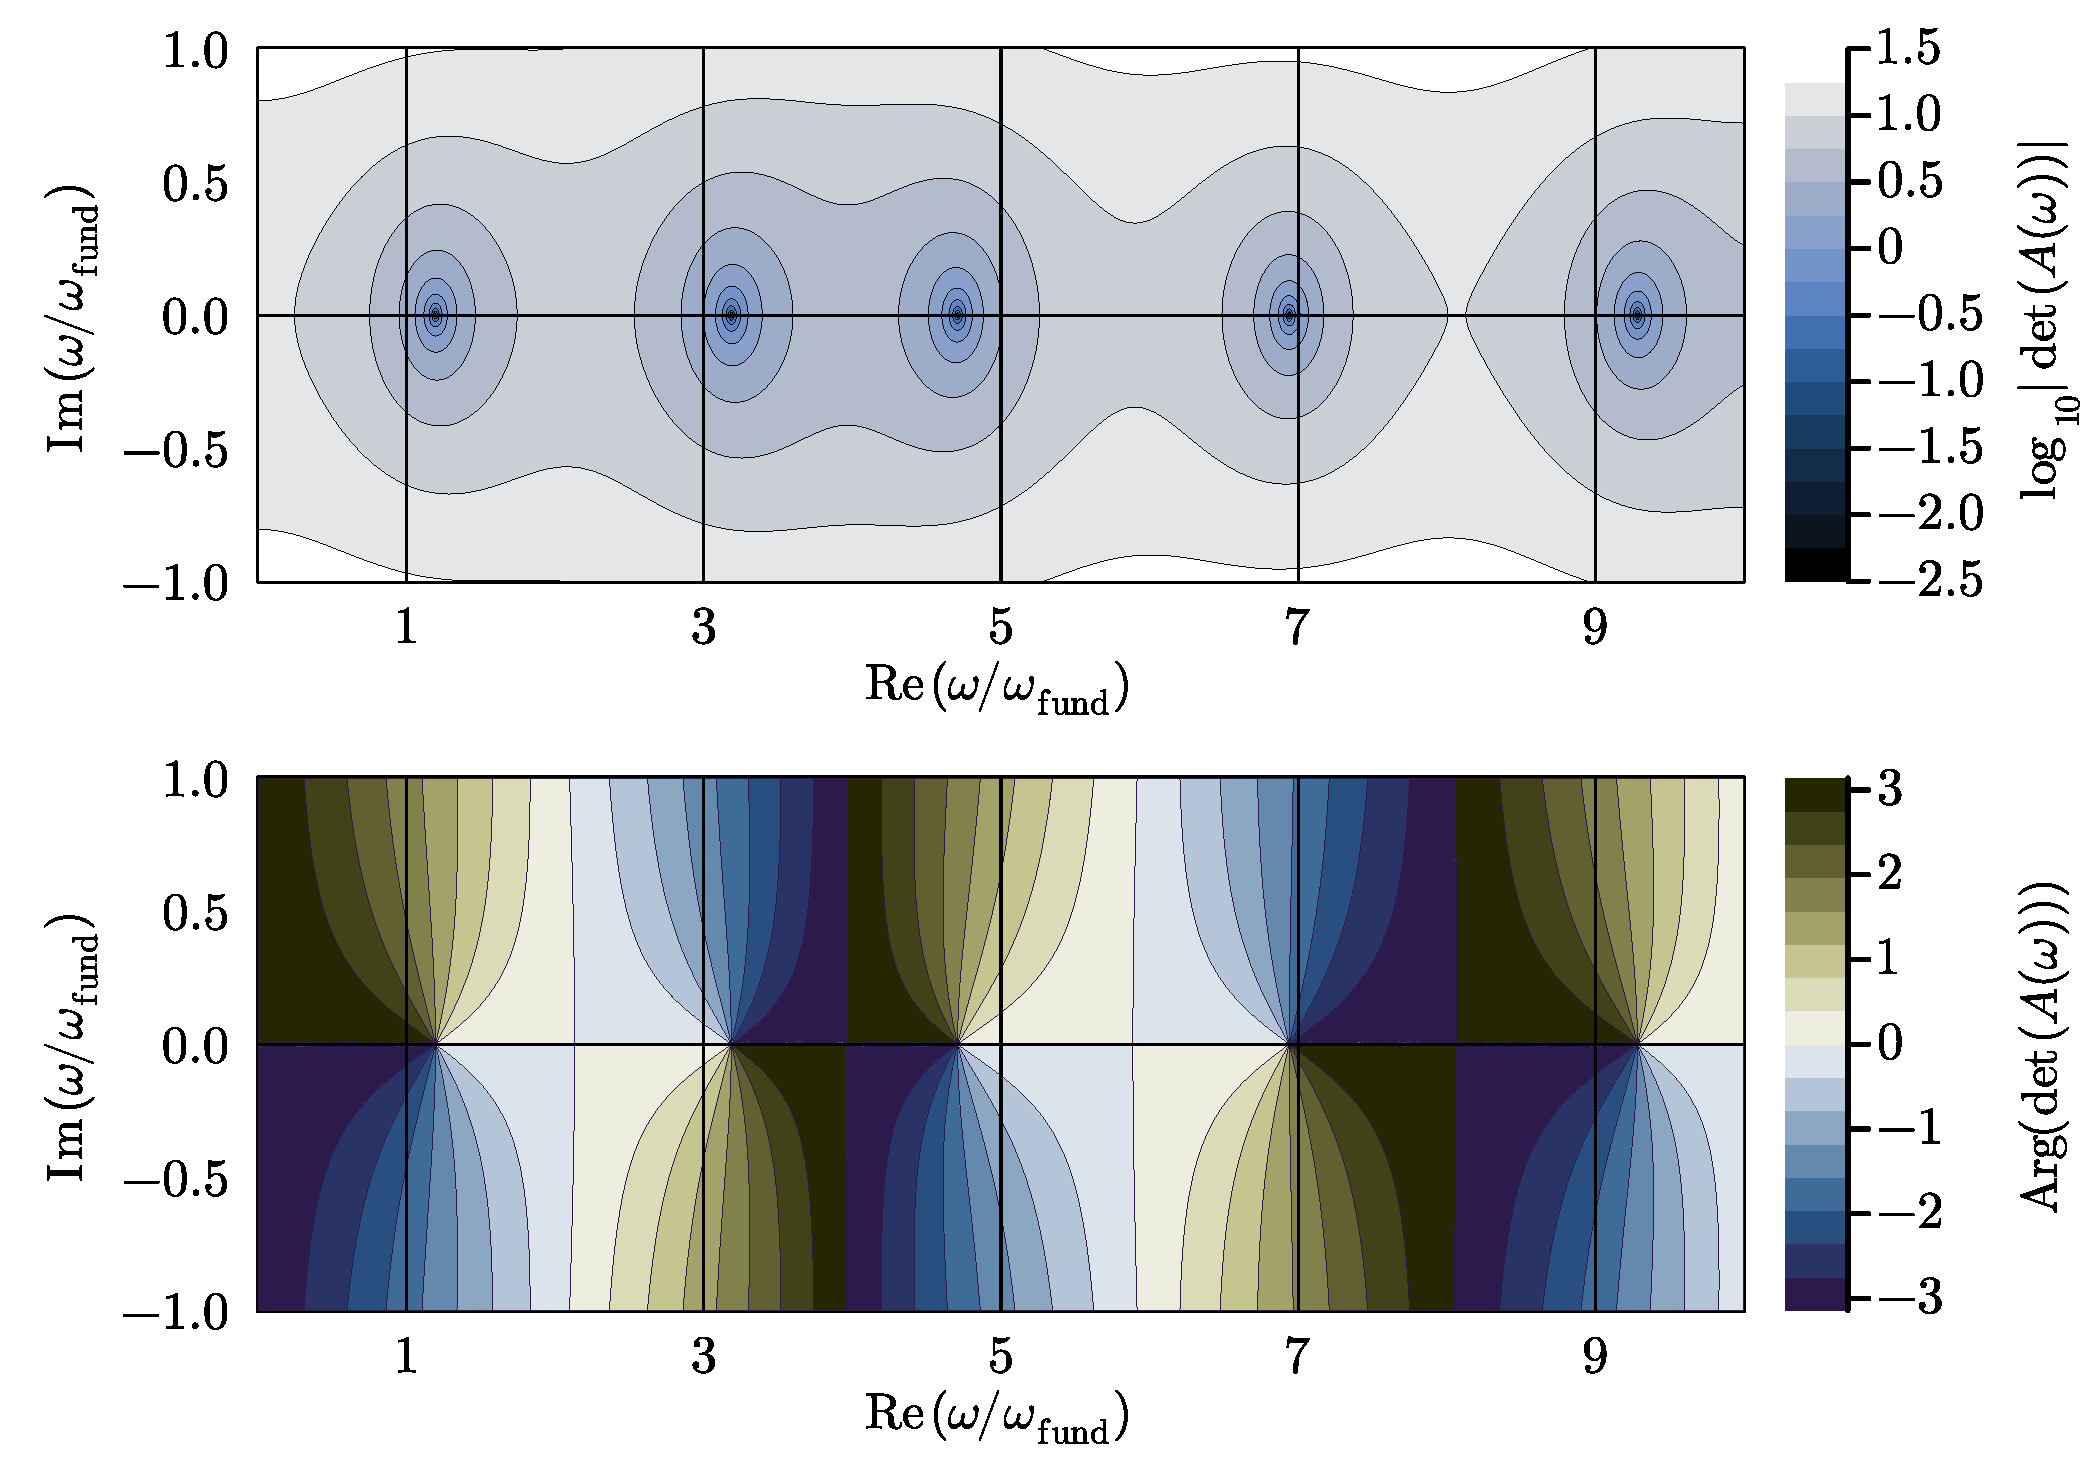
\includegraphics[scale=0.35]{assets/graphs/r=7_xf=05_complex_harmonics.pdf}
\caption{$r = 7, x_f = 0.5$, CAPTION}
\label{fig:flame-harmonics-complex}
\end{figure}

% For a flame which is .. and .., we expect harmonics of frequencies .. provided that the acoustics remain linear and are not interacting with the flame
% Note that this only accounts for the modes of a stationary density jump. If the flame is moving instead, the acoustic modes in the tube change with the moving flame. Hence the acoustics in the tube will be much more complex in this case in a way which is not predicted by this model. More complex control diagrams may be required to model the moving system instead.




\subsection{Results}

% Show some fields at an example time for both simulations

% stats data fft postprocessing/windowing

% spectrogram results

% frequencies

% mode structures!



\begin{figure}[t]
\centering
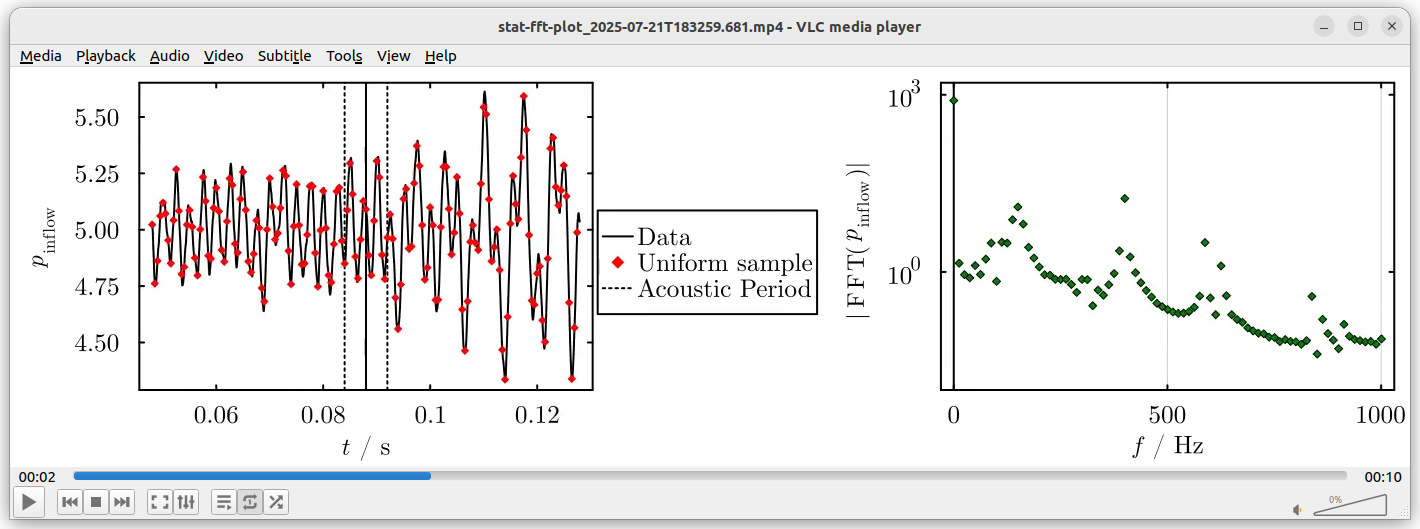
\includegraphics[scale=0.35]{assets/graphs/fft-windowing.png}
\caption{[PLACEHOLDER IMG] FFT WINDOWING}
\label{fig:windowing}
\end{figure}

\begin{figure}[t]
\centering
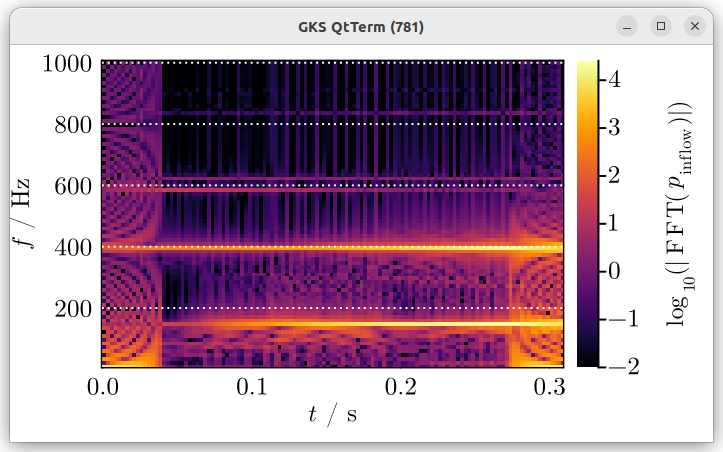
\includegraphics[scale=0.35]{assets/graphs/spectrogram.png}
\caption{[PLACEHOLDER IMG] SPECTROGRAM}
\label{fig:spectrogram}
\end{figure}

\begin{figure}[t]
\centering
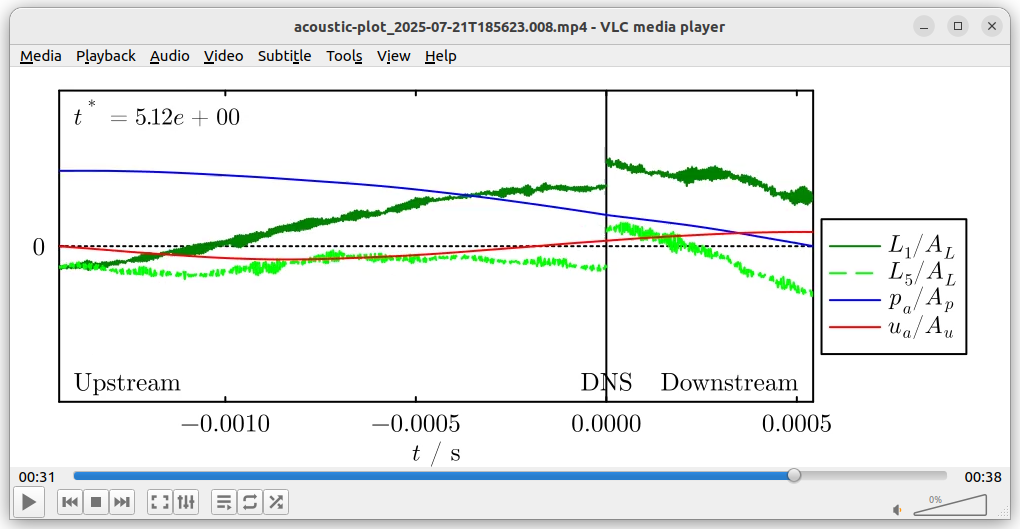
\includegraphics[scale=0.35]{assets/graphs/pp-tones.png}
\caption{[PLACEHOLDER IMG] POST-PROCESSED 1/4 AND 3/4 WAVE EVIDENCE}
\label{fig:pp-tones}
\end{figure}



\cleardoublepage

\chapter{Discussion} \label{ch:discuss}
\section{Comparison with D-TDIBC}

The work of \cite{douasbin2018DelayedtimeDomainImpedance} provides a similar one-dimensional model for outflow acoustics based on their associated time delay by means of an impedance boundary called delayed time-domain impedance boundary conditions (D-TDIBCs). The method itself is reviewed in \chap{ch:lit-review}; here we simply observe potential benefits and drawbacks of the ADCBC method against the D-TDIBC method. Most obviously, D-TDIBC offers and validates only an outflow boundary method where ADCBC provides arbitrary acoustic delays for any characteristic boundary -- although only inflows and outflows are practical and validated here. Also, boundary values in D-TDIBC are calculated from information in the previous time step, with no information stored about the acoustic region. Hence, it is not immediately possible to access and visualise the acoustics in this downstream region. By contrast, a method has been provided in the ADCBC case, where the sample queues are reinterpreted as upstream and downstream spatial data of acoustic $\cl{L}_{1/5}$ values. This comes at the cost of a much larger memory burden required by these queues which is placed only onto the boundary processors. This memory footprint is not present in D-TDIBC. In both methods a strongly one-dimensional flow is required at the boundary and only delay effects under linear acoustics are modelled, although the non-linear effects of impedance are implicitly involved in the impedance boundary formulation of D-TDIBC. This can be extended to model arbitrary reactions downstream boundaries to different frequencies in the envelope of the reflection coefficient. By comparison, ADCBC allows for other boundary treatments to potentially be `tacked on' by adding further terms to $\cl{L}_{1/5}(t)$. This has the natural benefit that the method should be easily implementable into systems already using an NSCBC formulation for non-reflecting boundaries. However, this has the drawback that the method is entirely reliant on the effectiveness of the baseline non-reflection. In both methods minimal cost is paid per step to apply the boundary conditions, but in the case of D-TDIBC a pre-processing cost must be paid to model a given time-delay and reflection coefficient envelope. Since no inflow formulation is given in their case, the movement of the DNS region through the physical domain would not be physical by means of changing the outflow delay, as we do with ADCBC.



\section{Report Conclusions}





\section{Future Work}

More immediate work ought to be done to further validate the proposed ADCBC method from \chap{ch:delay-bcs}, including investigating the interpolation of $\cl{L}_{1/5}$ values and ensuring that acoustic energy does not trivially increase over long time periods without a flame. Having said that, the method provides a framework for multiple different thermoacoustic applications, particularly for those taking place in long tubes. Thermodiffusive and thermoacoustically unstable flames can already be modelled with the caveat that the rapidly changing flame speeds of thermodiffusive flames likely mean it will exit the DNS domain. To remedy this, dynamic inflow velocities are required which do not couple to the acoustics and counteract the mean flame speed. This is also useful for other, non-thermodiffusive flames which reach secondary instability since the flame speed changes drastically under this regime. Another typical test case and one which is used to test the D-TDIBC method in \cite{douasbin2018DelayedtimeDomainImpedance} is a flame in a strong counterflow, held in place by an adiabatic cylindrical flame holder. Comparisons to their calculated eigenmodes could be found by simulating the same model geometry whilst also providing mode shapes in the fictitious domain. ADCBC should also be easily applicable to flames passing through arrays of cylinders (or other porous geometries). Typically, this is expensive to model due to the task of fitting the discretisation to the complex body and the large scale disparity in thermoacoustics. Utilising the LABFM discretisation in the SUNSET code coupled to low-order ADCBC allows us to model this phenomena for the cost of discretising only the flame and its surrounding hydrodynamic region.

Furthermore, the use of characteristic boundaries allows us to freely impose incoming acoustics through the inflow, $\cl{L}_{5, \rm{imposed}}(t)$ and outflow, $\cl{L}_{1, \rm{imposed}}(t)$ on top of their existing values from the acoustic delay. By implementing an imposed e.g. sinusoidal forcing to model an upstream loudspeaker playing a pure tone, we can trigger secondary instabilities in a model version of \cite{searby1991ParametricAcousticInstability}. This would allow us to more efficiently investigate secondary instability modes and their flame structures. This could be potentially elaborated into three dimensions to try and recreate the wavenumber measurements of \cite{delfin2024DeterminationMethodMarkstein}. Turbulent flow can also be imposed through the VFCBC method established in \cite{guezennec2009AcousticallyNonreflectingReflecting} and an attempt could be made to implement this on top of the existing ADCBC method, as above. Turbulent characteristic outflows would also need to be implemented for compatibility. This may allow us to simulate faster flows in broader domains which are expected to be turbulent, as well as potentially allowing us to observe the self-turbulent flames seen resulting from secondary instability in \cite{searby1992AcousticInstabilityPremixed}.

Thus far, we have gotten away with values of $\abs{R_{\rm{U}/\rm{D}}} = 1$, but more realistic boundaries have impedances which vary with frequency. Could this be explored using some predefined spectral filtering on the delayed $\cl{L}_{1/5}$ values? Practically speaking, a low-pass filter could be used to remove high-frequency noise and improve the quality of observed low frequency modes (at the cost of precluding high-frequency ones). More generally, the non-linear acoustic effects which are not being modelled here could be included by coupling an acoustic solver to the DNS inflow and outflow. Using for example a boundary element method or analytical techniques, acoustics around some up- or downstream geometry can be solved for in tandem with the DNS domain. This could enable us to simulate a flame tube with a porous plug and compare to the analysis of \cite{gaton-perez2025MitigationThermoacousticInstabilities}.



\section{Planning}

\begin{figure}[t]
\centering
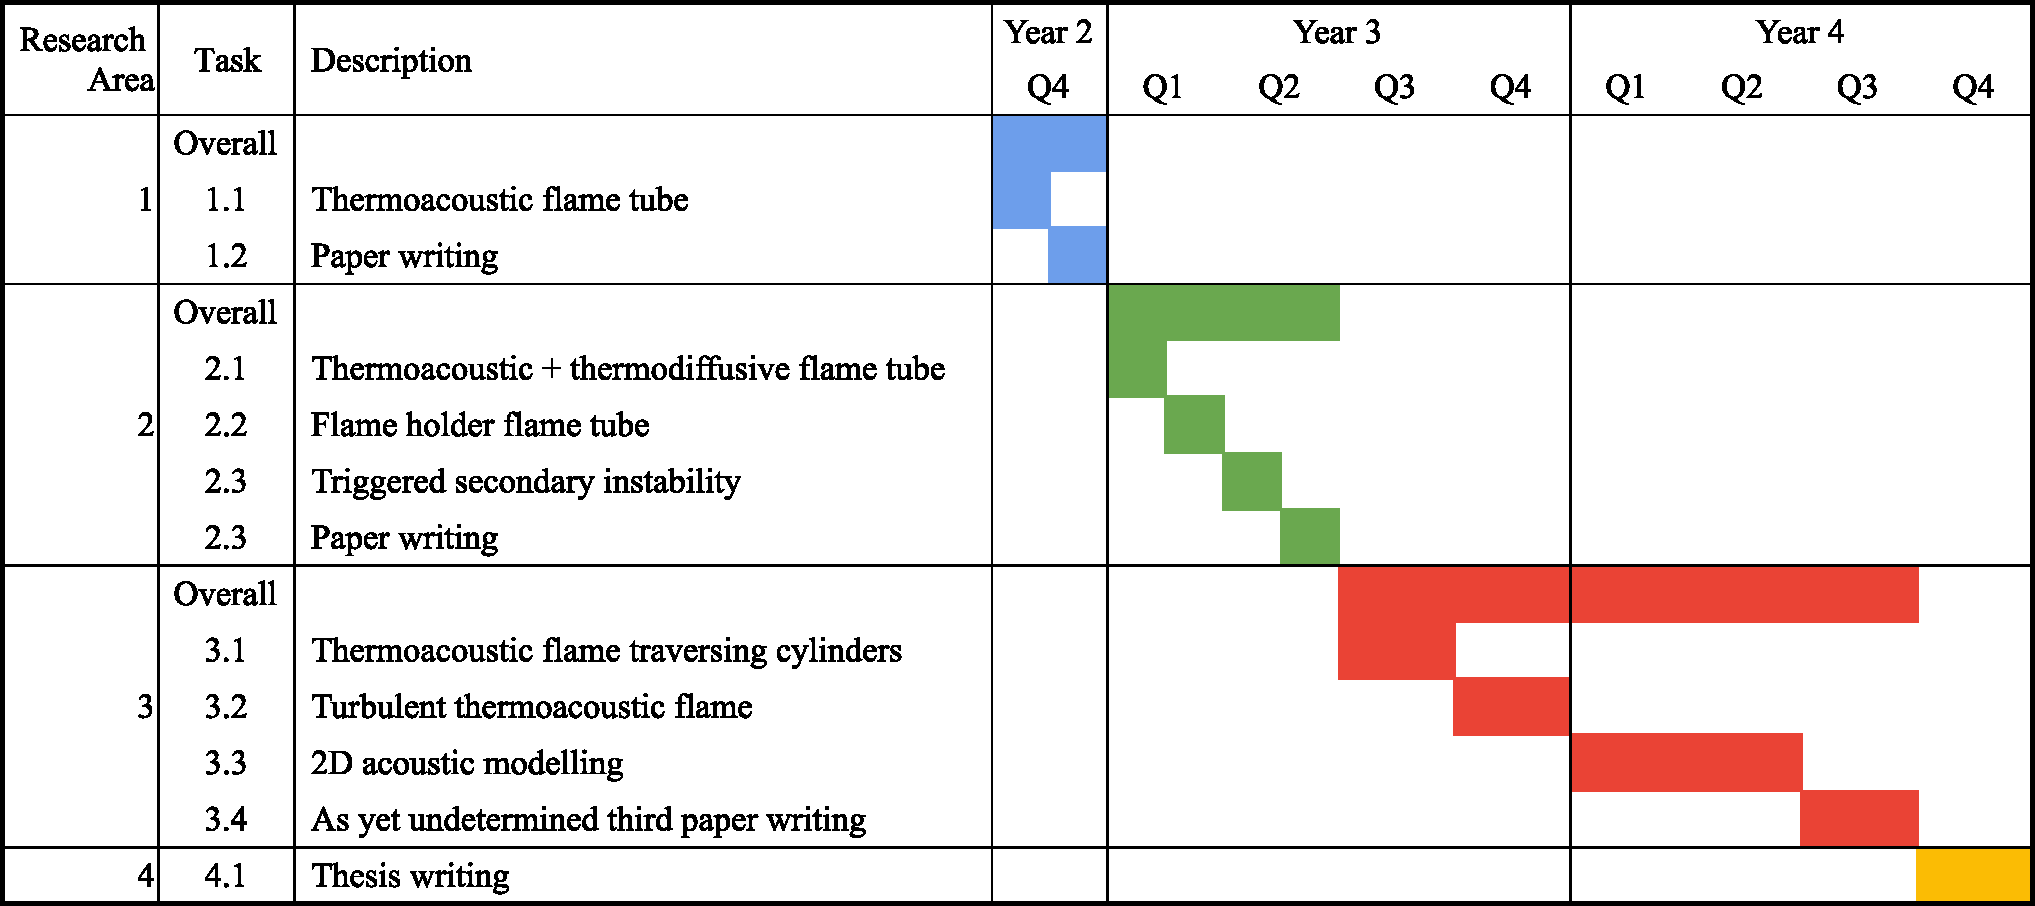
\includegraphics[scale=0.5]{assets/graphs/2YR_Gantt.pdf}
\caption{Gantt chart organising tasks for the remaining seven quarters of my PhD.}
\label{fig:gantt}
\end{figure}

There are seven quarters left before my thesis must be written and submitted and the three and a half years of my PhD, beginning January 2024, are over. Currently, I am organising future work into the journal articles (papers) they fit into and timetabling these tasks accordingly:
\setlist[enumerate]{label={\arabic*.}}
\begin{enumerate}
\item \textbf{Paper 1. One quarter needed total.} This paper will focus on the ADCBC method, with examples of an acoustic bump, acoustic standing wave and thermoacoustic flame tube. The method will be explained alongside post-processing for the acoustic domain.
    \begin{enumerate}
    \item Completion of the simulation, post-processing and analysis of a thermoacoustic flame tube for a journal article has yet to be fully done. Primarily due to the analysis, which will be used for further thermoacoustic simulations, half a quarter is needed. Calculations of Rayleigh Indices, RI and acoustic envelopes need to be performed and the aforementioned interpolation issue needs to be investigated
    \item The rest of the quarter will be used to write the paper.
    \end{enumerate}
\item \textbf{Paper 2. Two quarters needed total.} This paper will focus on applications of the ADCBC method to simulations of various physical phenomena, each of which do not require large developments of the ADCBC method.
    \begin{enumerate}
    \item A thermodiffusive and thermoacoustically unstable flame require dynamic inflow non-acoustic velocities. Alongside simulations, post-processing and analysis I estimate this to take half a quarter.
    \item Similarly, a counterflow flame holder flame might require some extra work to implement the correct physical initial conditions for a simulation using ADCBC restarted from an unsteady simulation using non-reflecting NSCBC. I estimate this to take half a quarter too.
    \item The final phenomena is a simulated secondary thermoacoustic instability, which relies on the prior work to change inflow speeds dynamically and impose an additional acoustic field, as mentioned above. I estimate this to take half a quarter too.
    \item The rest of the two quarters will be used to write the paper.
    \end{enumerate}
\item \textbf{Potential third paper. Four quarters needed total.} This paper not yet in focus and its specific contents will be determined by the remaining time and feasibility of each individual task.
    \begin{enumerate}
    \item Simulation of a thermoacoustically unstable flame travelling through arrays of cylinders in a broader domain will likely take a quarter, since I may have to introduce a queue system for each boundary node and perform three-dimensional simulations.
    \item The aforementioned self-turbulent thermoacoustically unstable flame simulation also requires development of the ADCBC to be compliant with turbulent flows and is estimated to take a quarter.
    \item I suspect investigations into more elaborate acoustic modelling will be a deeper rabbit hole, which could take a long time if it is provided. By restricting the scope to what is reasonable to do in the rest of my PhD, I estimate it should only take one quarter.
    \item The rest of the four quarters will be used to write a paper from the resulting research.
    \end{enumerate}
\item \textbf{Thesis. Two quarters needed total.} This should be written in conjunction with the above to make the best use of time.
    \begin{enumerate}
    \item As mentioned, my thesis must be written by the end of 2027 and I estimate it will take roughly one quarter to put together alongside other work.
    \end{enumerate}
\end{enumerate}
This is organised into a Gantt chart in \fig{fig:gantt}, showing how the remaining nine quarters will be used in sequence. Further up-to-date details on this plan are given at \href{https://www.dropbox.com/scl/fi/4w62xppcfkywnr7nm8a6v/plan-Y3.md?rlkey=yx4ez0nmqjaabqseotnzfiqsn&st=lll313fe&dl=0}{\texttt{this link}}.



\cleardoublepage

\colorlet{benlinkcol}{black}
\colorlet{benurlcol}{black}
\printbibliography[title={References}, heading=bibintoc]


\end{document}
